\section{Motivation}
As introduced earlier, the most direct probes of the top quark Yukawa coupling, $y_{t}$, are provided by the associated production of a Higgs boson with either a top--antitop quark pair ($t\bar{t}H$) or a single top quark ($tH$). 
While the $t\bar{t}H$ process, discussed in detail in Chapter~\ref{chap:htautau}, is primarily sensitive to the absolute magnitude of $y_{t}$, the $tH$ process is unique in that it also probes the relative sign of the coupling~\cite{Tait_2000,Barger_2010,Biswas_2013,Farina_2013,Chang_2014}. 
This difference originates from the interplay between diagrams in which the Higgs boson couples directly to the top quark and those in which it couples to the $W$ boson. 
In $tH$ production, these two contributions interfere, such that the overall cross section depends not only on $|y_{t}|$ but also on its sign relative to the Higgs--$W$ coupling. 
The nature of the interference, however, depends strongly on the production mode. 
In the $t$-channel ($tHqb$), the interference is strongly destructive, which suppresses the cross section well below the sum of the individual contributions and makes this channel particularly sensitive to deviations from the SM prediction. 
In contrast, in the $s$-channel the interference is constructive, leading to a total cross section larger than that of the individual diagrams, although its absolute rate remains very small.
For the $tWH$ process the interference is also destructive, but its impact is less pronounced than in the $t$-channel. 
As a result, each of these channels probes the top-Higgs interaction in a different way, with the $t$-channel providing the highest sensitivity to the sign of $y_t$. 
The corresponding Feynman diagrams, illustrating the contributions from the Higgs-top and Higgs-$W$ couplings and their interference in the different modes, are shown in Figures~\ref{fig:feynman_tH_t},~\ref{fig:feynman_tH_s} and~\ref{fig:feynman_tWH}.

\begin{figure}[htbp]
    \centering
    \begin{subfigure}[b]{0.4\textwidth}
      \centering
      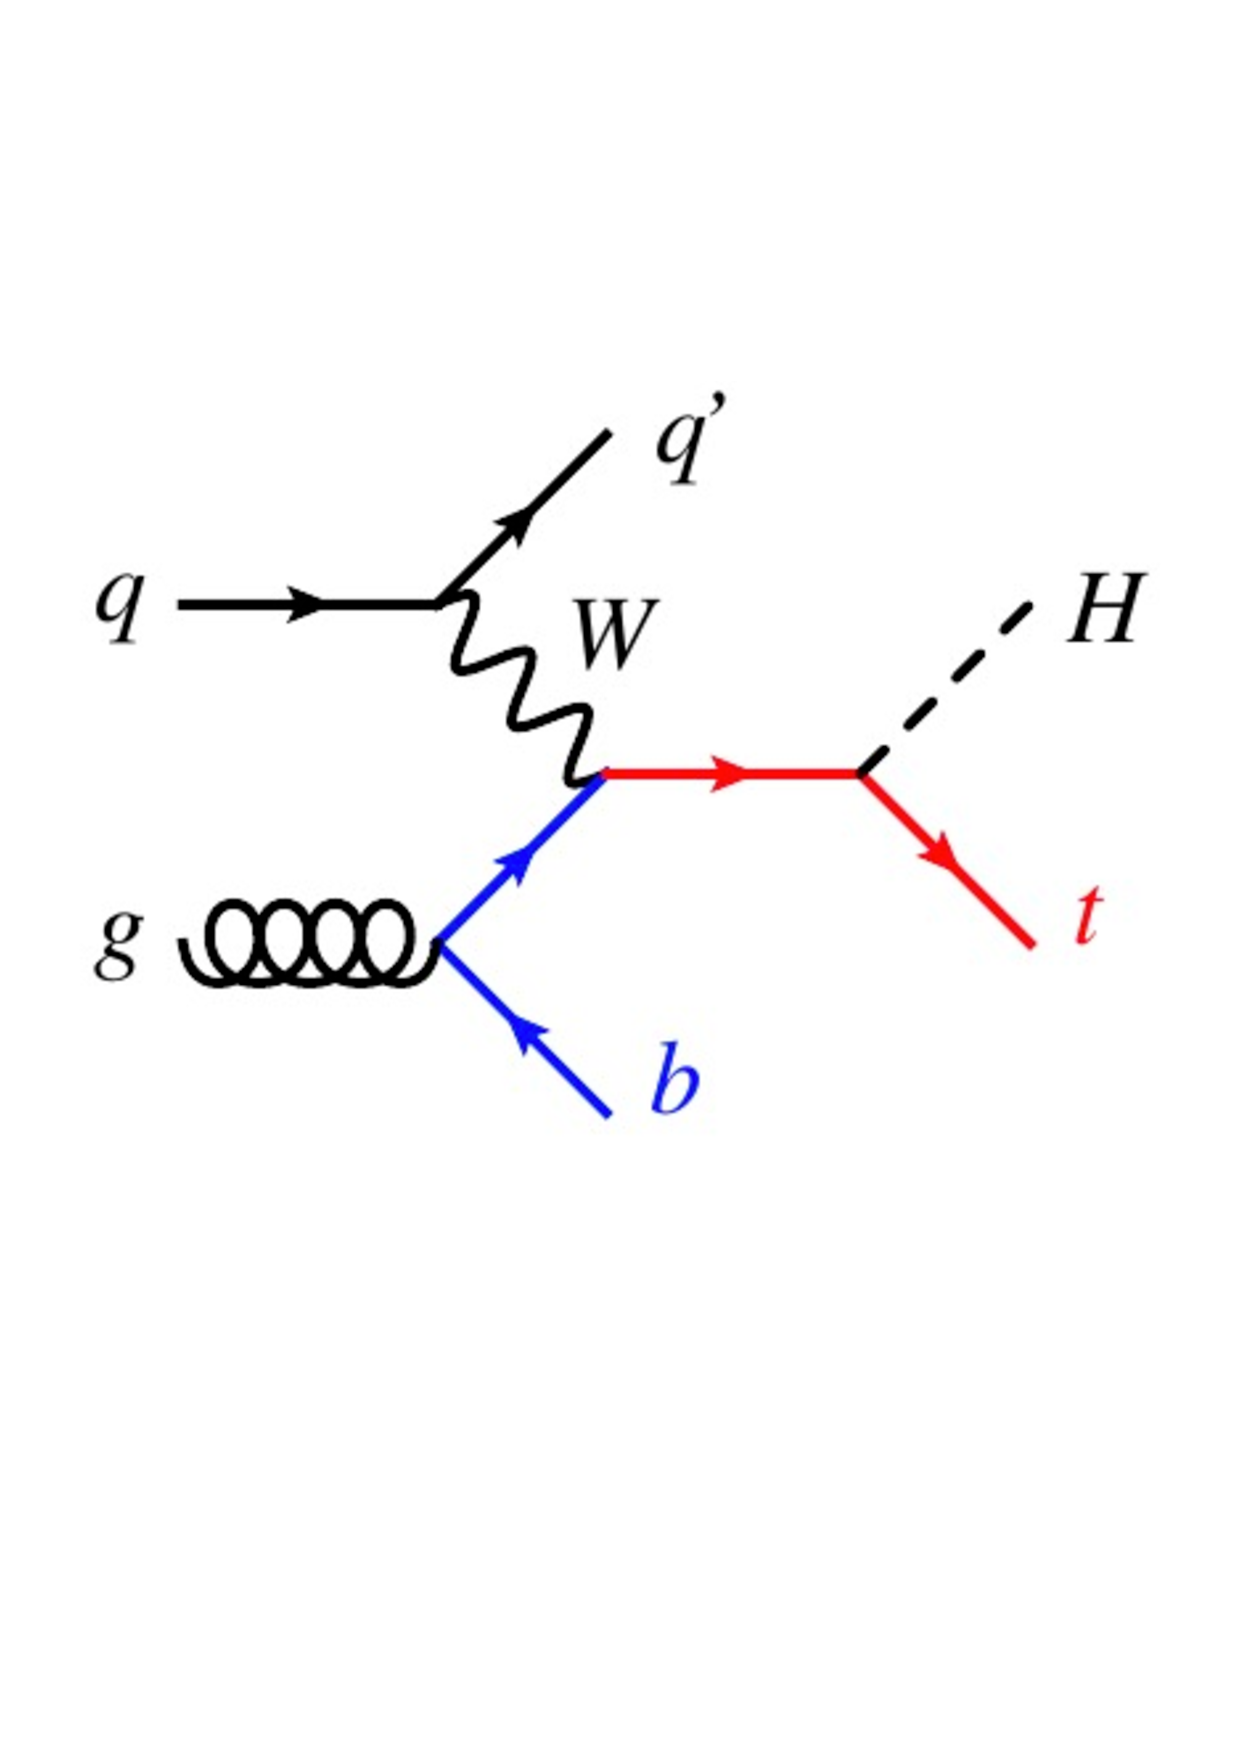
\includegraphics[width=\textwidth]{thqb_t}
    \end{subfigure}
    \begin{subfigure}[b]{0.4\textwidth}
      \centering
      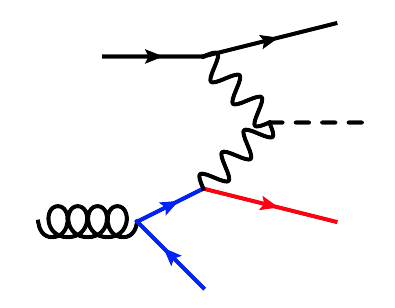
\includegraphics[width=\textwidth]{thqb_t_2}
    \end{subfigure}
    \caption{Representative leading-order Feynman diagrams for $tHqb$ in the $t$-channel~\cite{Barger_2010}.}
    \label{fig:feynman_tH_t}
  \end{figure}


  \begin{figure}[htbp]
    \centering
    \begin{subfigure}[b]{0.4\textwidth}
      \centering
      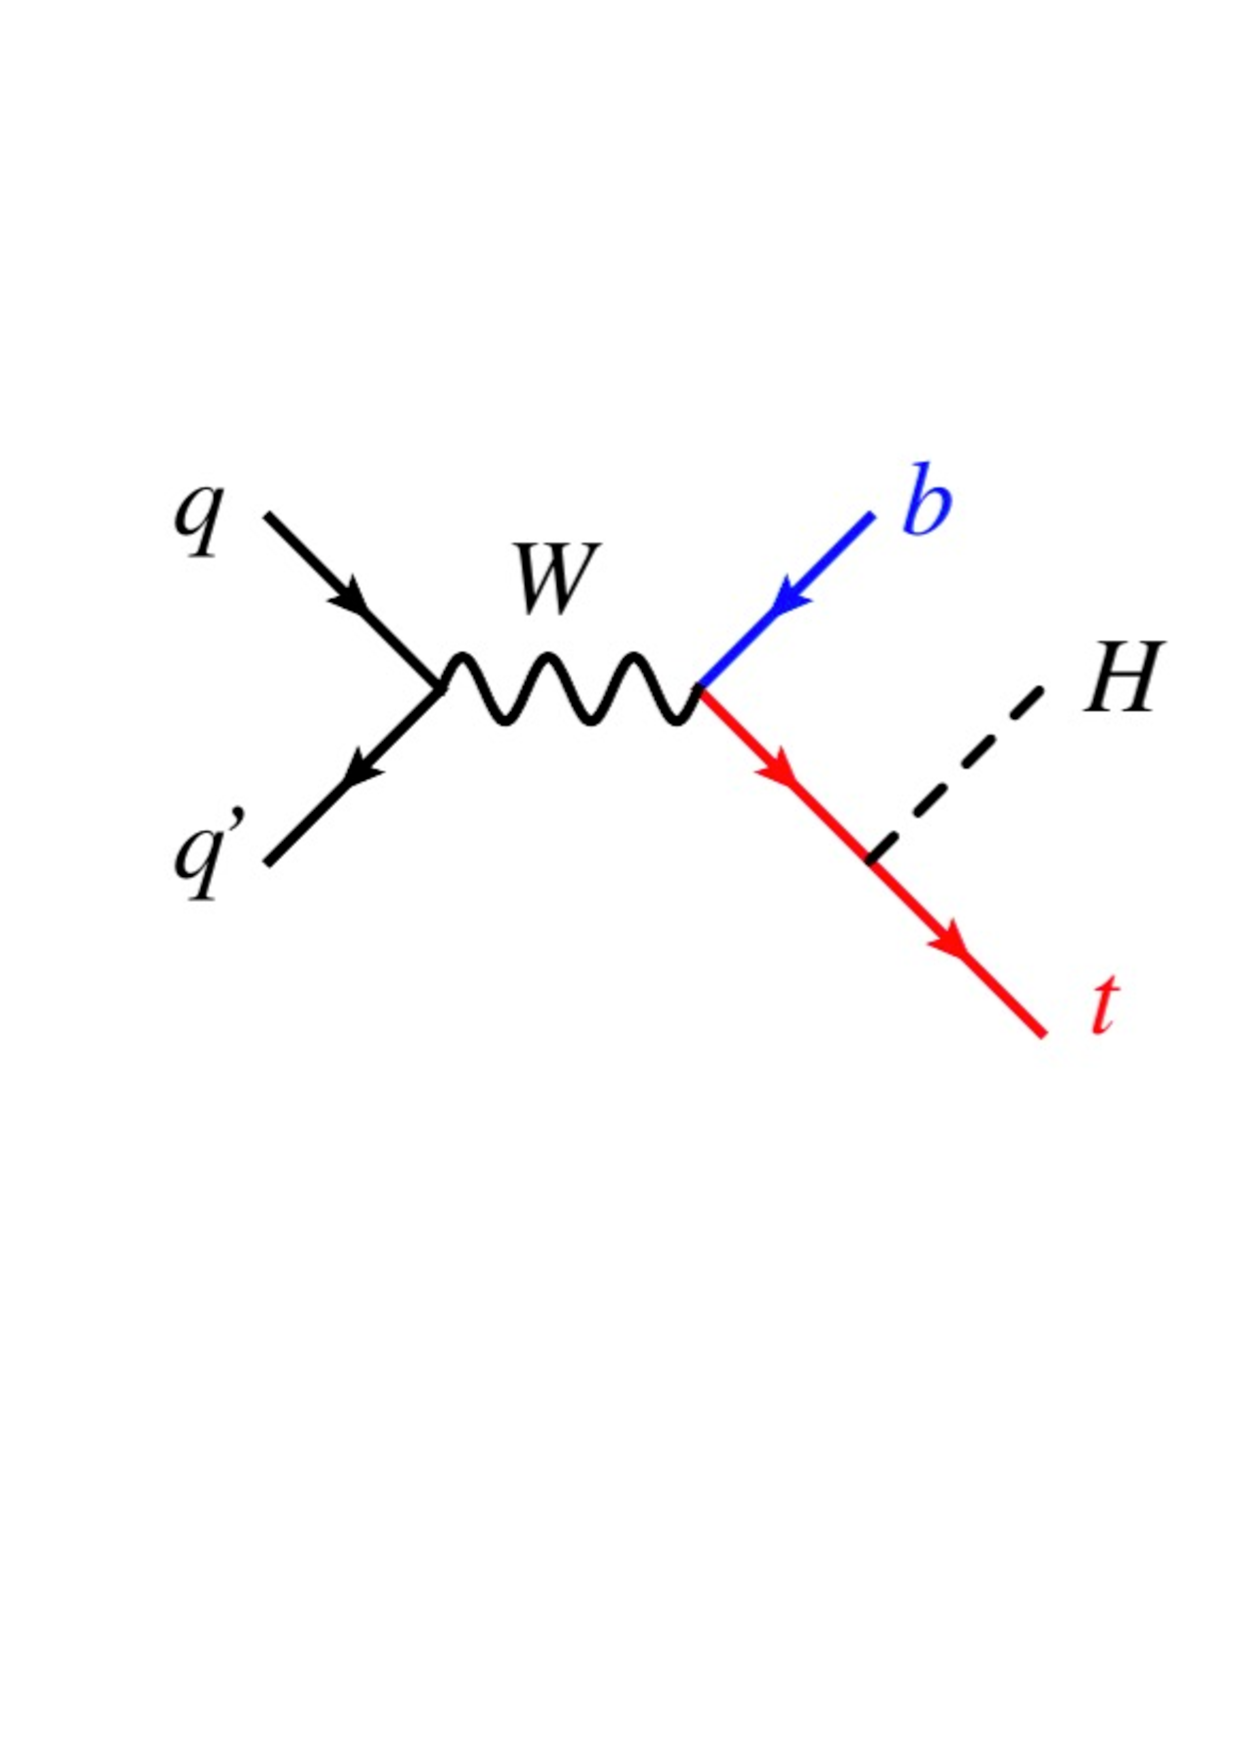
\includegraphics[width=\textwidth]{thqb_s}
    \end{subfigure}
    \begin{subfigure}[b]{0.4\textwidth}
      \centering
      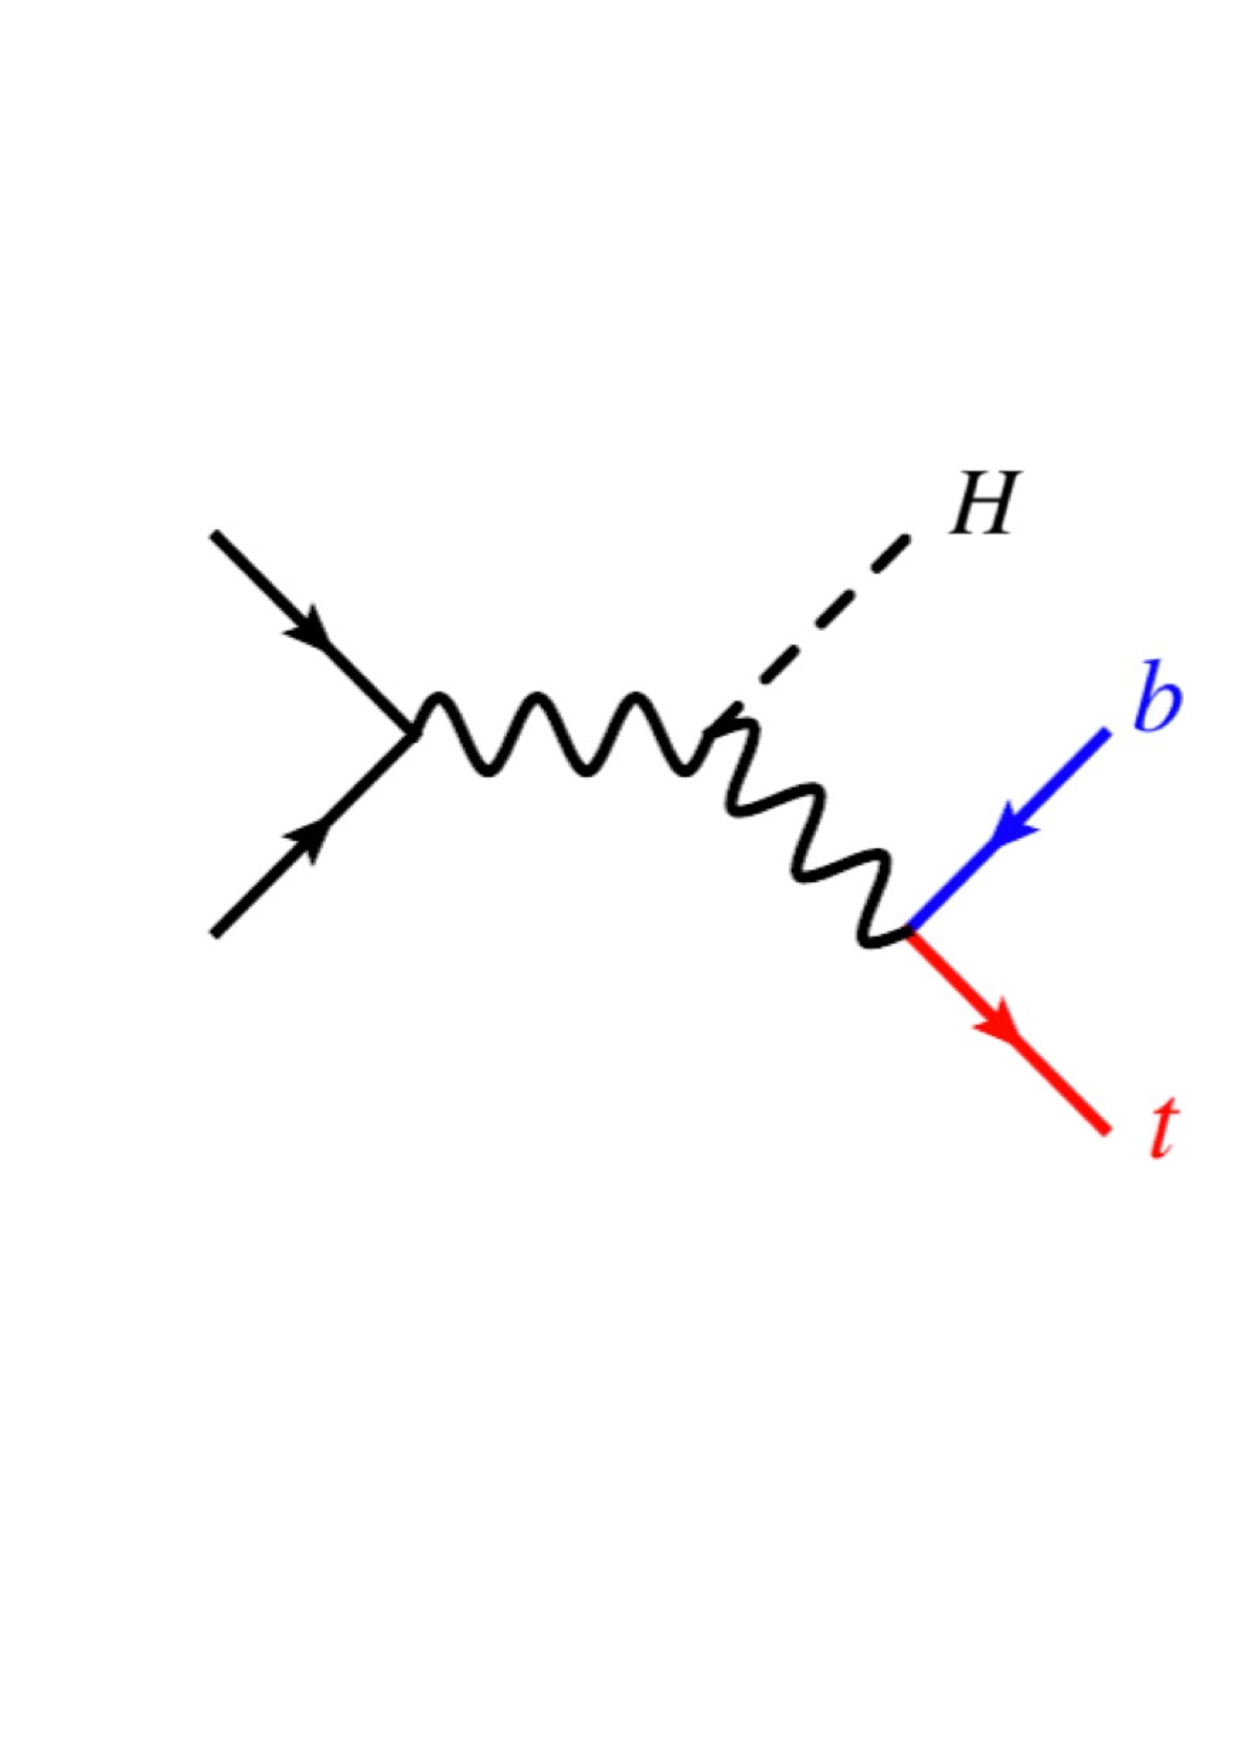
\includegraphics[width=\textwidth]{thqb_s_2}
    \end{subfigure}
    \caption{Representative leading-order Feynman diagrams for $tHqb$ in the $s$-channel~\cite{Barger_2010}.}
    \label{fig:feynman_tH_s}
  \end{figure}

\begin{figure}[htbp]
    \centering
    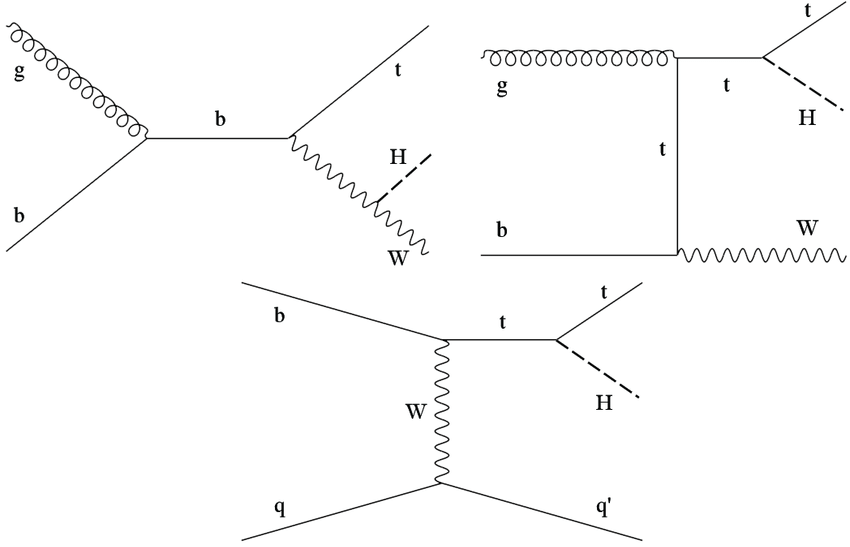
\includegraphics[width=0.6\textwidth]{twh.png}
    \caption{Representative leading-order Feynman diagrams for $tWH$~\cite{twh}.}
    \label{fig:feynman_tWH}
  \end{figure}

If the sign of $y_{t}$ were opposite to the SM prediction, the destructive interference in the $t$-channel would turn constructive, enhancing the cross section by up to an order of magnitude and potentially resulting in an observable excess of events. 
This makes $tH$ production a powerful and complementary probe to $t\bar{t}H$. 
Whereas $t\bar{t}H$ establishes the presence of the Yukawa interaction and constrains its absolute strength, $tH$ is directly sensitive to its relative phase, providing access to possible deviations such as a flipped sign or $CP$-mixed structures. 
  
  
  The production of a Higgs boson in association with a single top quark proceeds via the electroweak interaction, with three main modes contributing at the LHC: the $t$-channel ($tHqb$), the $s$-channel ($tHb$), and the associated production with a $W$ boson ($tHW$)~\cite{demartin2015higgsproductionassociationsingle,Demartin_2017}. 
  The $t$-channel is by far the most relevant, with a predicted cross-section of about $74$~fb at $\sqrt{s}=13$~TeV, compared to $15$~fb for $tHW$ and less than $3$~fb for the $s$-channel. 
  Experimentally, the $tHW$ process is characterised by a distinct topology due to the additional $W$ boson in the final state, and is therefore treated as a background in searches for $tHqb$. 
  For this reason, the present work focuses on the $tHqb$ process in the hadronic $H\to\tau_{\mathrm{had}}\tau_{\mathrm{had}}$ final state, which is directly comparable to the $t\bar{t}H$ topology. 
  
  The $tHq$ event topology is characterised by two heavy objects, namely a top quark and a Higgs boson radiated from the former, accompanied by an energetic light-flavour quark (predominantly a $u$- or $\bar{d}$-quark) and an additional soft $b$-quark originating from gluon splitting. 
  The top-quark and Higgs-boson systems are typically produced in the central region of the detector, recoiling against each other. 
  In contrast, $tWH$ production features three heavy objects in the final state: the top quark, a $W$ boson, and a Higgs boson radiated from either of these particles, together with a soft $b$-quark from gluon splitting. 
  This topology closely resembles $t\bar{t}H$ production and results in an identical final state, making it difficult to disentangle from the $t\bar{t}H$ contribution and therefore treated as a background in this analysis. 
  
  So far, single-top Higgs production has not been observed. 
  The CMS Collaboration has reported upper limits on the $tH$ rate in both multi-lepton and $b\bar{b}$ final states. 
  In the multi-lepton channel, the measured signal strength was found to be 
  \[
  \mu_{tHqb+tWH} = 5.1 \pm 2.7~(\text{stat.}) \pm 3.0~(\text{syst.})~\cite{Sirunyan_2021},
  \] 
  while in the $b\bar{b}$ channel cross-sections up to 14.6 times the SM prediction were excluded at 95\% confidence level~\cite{2025}. 
  The most recent ATLAS search, based on the full Run-2 dataset and targeting $H\to b\bar{b}$, $H\to WW^*$, $H\to ZZ^*$, and $H\to\tau\tau$ decays in events with an isolated lepton from the top quark, reports a measured signal strength of
  \[
  \mu_{tH} = 8.1 \pm 2.6~(\text{stat.}) \pm 2.0~(\text{syst.}),
  \] 
  corresponding to a 2.8\,$\sigma$ observed (0.4\,$\sigma$ expected) significance above the background-only hypothesis. 
  The observed (expected) 95\% confidence level upper limit on the $tH$ cross-section was $13.9$ ($6.1$) times the SM prediction~\cite{ATLAS:2025irr}. 
  This represents the most stringent constraint on $tH$ production to date, while still allowing for possible deviations from the SM. 
  
  In this context, the hadronic di-$\tau$ final state provides an attractive and complementary probe of both $t\bar{t}H$ and $tHqb$ production. 
  In particular, no ATLAS analysis has yet targeted the $tHqb$ channel in the absence of electrons or muons. 
  Moreover, a combined measurement is especially well motivated given that, due to their similar topology, $t\bar{t}H$ and $tHqb$ share the same dominant backgrounds, namely $Z\to\tau\tau$+jets and $t\bar{t}$. 
  Such a joint analysis becomes feasible for the first time thanks to the larger dataset now available: by combining the full Run-2 dataset with the new Run-3 data, the statistical power of the search can be significantly enhanced. 
  This increase in luminosity, together with the adoption of improved object reconstruction and identification techniques, opens the possibility to explore $tHqb$ production in the $H\to\tau_{\mathrm{had}}\tau_{\mathrm{had}}$ final state with unprecedented sensitivity while simultaneously refining the measurement of $t\bar{t}H$.
  



\section{Analysis overview}

In this new study, the full Run-2 dataset is employed, corresponding to an integrated luminosity of $140$~fb$^{-1}$ at a centre-of-mass energy of $\sqrt{s}=13$~TeV, reprocessed with ATLAS software release 22. 
This dataset has been complemented with the Run-3 data collected to date, corresponding to an additional $166$~fb$^{-1}$ of luminosity from the years 2022-2024 of data taking, at a centre-of-mass energy of $\sqrt{s}=13.6$~TeV.
The increased statistical power provided by this combined dataset is one of the main motivations for exploring the $tHqb$ process together with $t\bar{t}H$ in the hadronic di-$\tau$ final state. 

Nevertheless, single-top Higgs production still suffers from low acceptance, particularly within the restricted phase space targeted in the previous $t\bar{t}H(\tau\tau)$ analysis presented in Chapter~\ref{chap:htautau}. 
In that context, the nominal signal topology involved six jets, with at least two $b$-tagged jets. 
The baseline selection was relaxed to five jets with at least two $b$-tags, or alternatively six jets with at least one $b$-tag, in order to recover acceptance lost due to $b$-tagging inefficiencies, with the expectation that the sensitivity would be recovered using MVA techniques. 

For $tHqb$, the selection must be relaxed even further. 
Nominally, this process yields 5 jets, of which two are expected to be $b$-tagged. 
With the release 22 of ATLAS software, however, novel identification algorithms have been introduced, including \textsc{GNTau} for $\tau$-lepton reconstruction and \textsc{GNv02} for flavour tagging of jets. 
These improvements, together with a refined MVA strategy, allow the analysis to maintain a good balance between efficiency and background rejection, even under looser jet requirements. 
The updated BDT strategy now targets two signal processes, $t\bar{t}H$ and $tHqb$, against the dominant backgrounds, $Z\to\tau\tau$+jets and $t\bar{t}$. 
This constitutes the first attempt within ATLAS to perform a simultaneous measurement of both processes in the fully hadronic $\tau\tau$ final state. 

The primary goal of this chapter is not to refine the measurement of the $t\bar{t}H$ cross section, but to study and quantify the sensitivity that can be achieved for $tHqb$ production using the additional Run-3 data. 
For this reason, no STXS interpretation is attempted here, in contrast to the previous $t\bar{t}H$ analysis. 
Instead, the final result presented in this chapter is the expected sensitivity derived from a statistical fit to pseudo-data samples, combined with real collision data in dedicated control regions used to validate the modelling of the dominant background processes. 
As in the previous analysis, the main backgrounds are modelled with Monte Carlo simulation and normalised to data through the fit, while fake-$\tau$ contributions are estimated with a fully data-driven fake-factor method. 
Overall, the same challenges and limitations encountered in the $t\bar{t}H(\tau\tau)$ analysis, such as the accurate modelling of $Z\to\tau\tau$+jets, the treatment of $t\bar{t}$ backgrounds, and the control of systematic uncertainties, are inherited here.

It is worth noting that, for the Run-3 MC simulations of \ttbar and \ztautau, significant mismodellings with respect to data are observed, particularly in the latter due to the change of generator version, as already discussed in Section~\ref{subsec:higgs_mc}. 
Following the same strategy as in the previous section, these discrepancies are ultimately corrected by dedicated normalization factors (NFs) that constrain and adjust the normalization of these backgrounds using data in the statistical fit. 
Nevertheless, in order to demonstrate that the overall agreement of the various observables, as well as the estimation of misidentified \tauhad backgrounds between MC and data, is under control, the \ttbar and \ztautau MC samples are rescaled by global factors of 1.3 and 1.4, respectively, in all distributions (unless otherwise stated). 
As will be shown later in Section~\ref{statistical_th_tth}, the normalization factors extracted from the statistical fit are consistent with these estimates. 
Figure~\ref{mmc_scaled} shows the distribution of \mmc in Run-3 at preselection level, before and after applying these scalings.

\begin{figure}[htbp]
    \centering
    \begin{subfigure}[b]{0.49\textwidth}
      \centering
      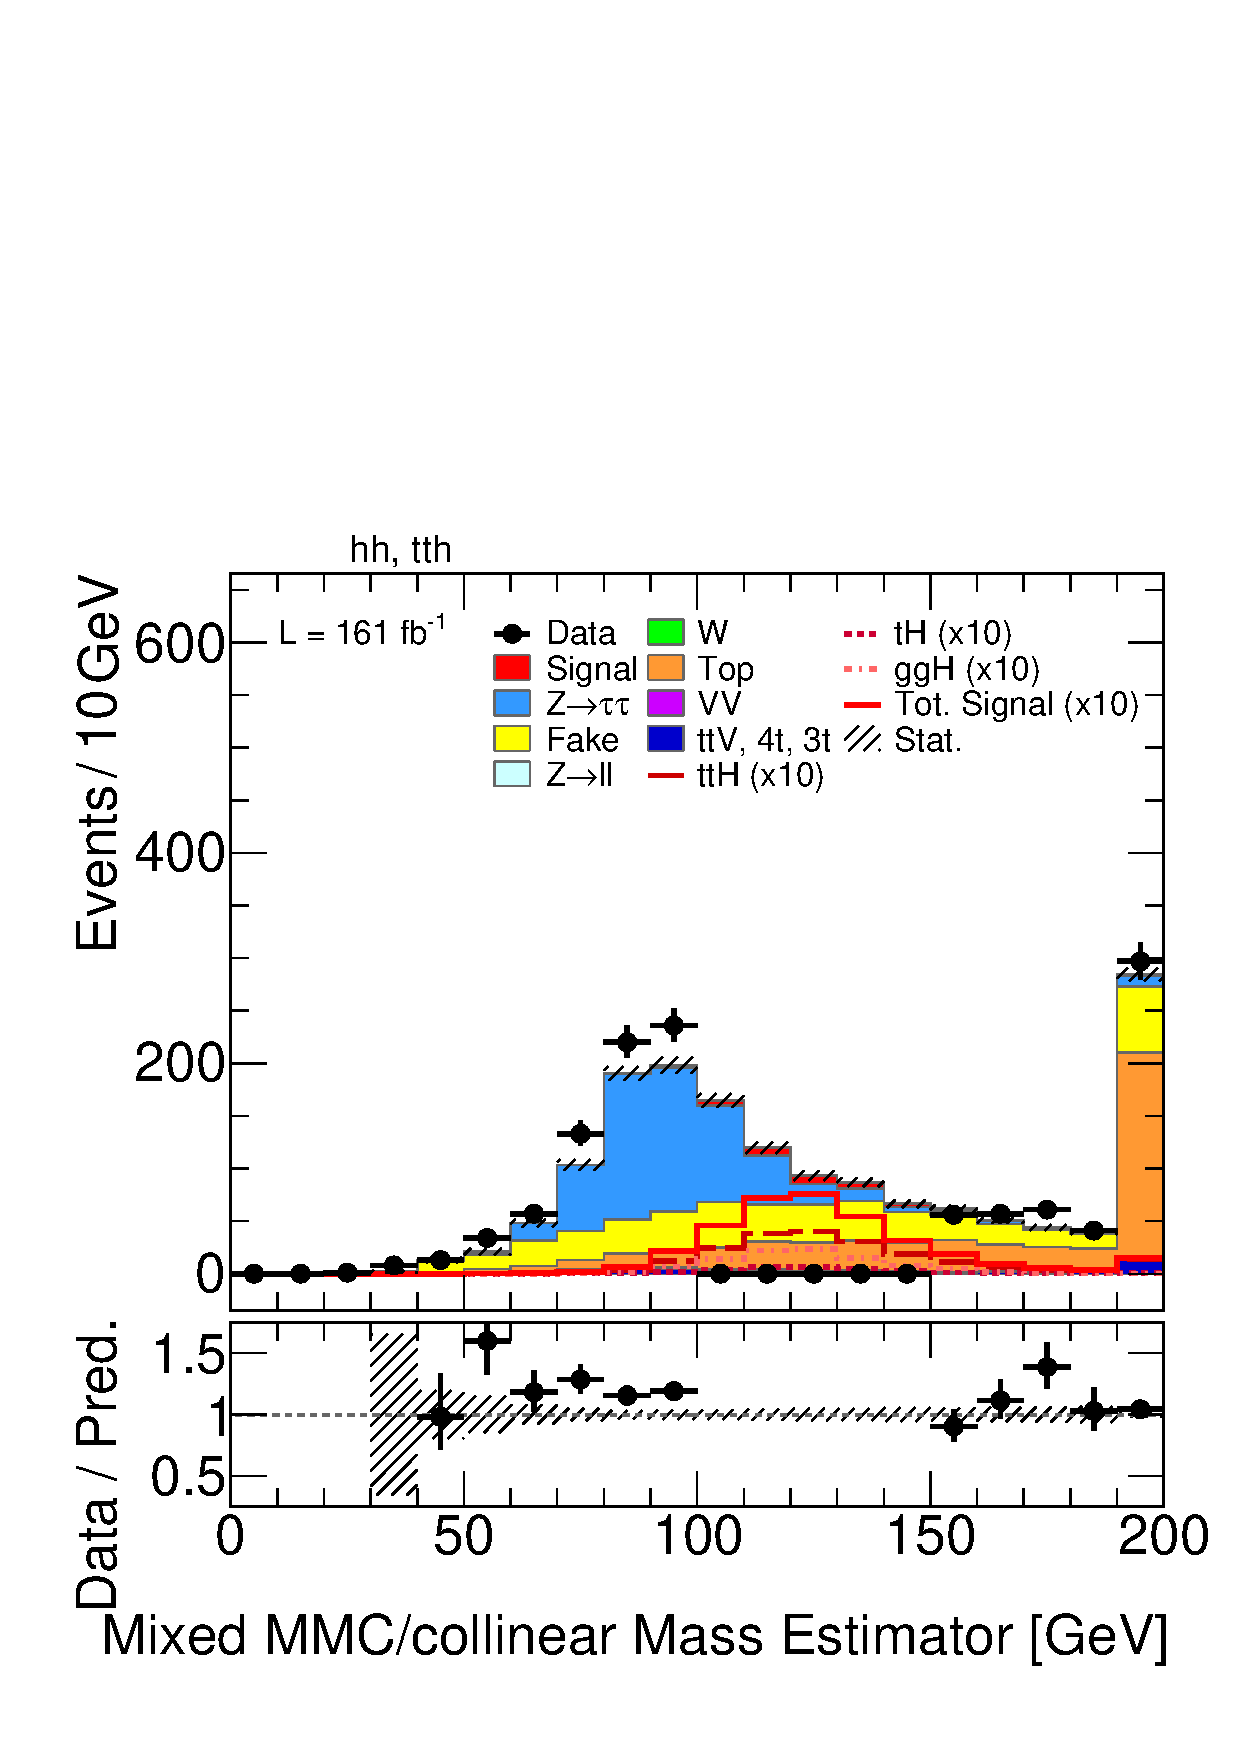
\includegraphics[width=\textwidth]{noscaled_plot_ditau_mmc_mlm_m_fix_hh_tth_22_23_24.pdf}
      \caption{}
    \end{subfigure}
    \hfill
    \begin{subfigure}[b]{0.49\textwidth}
      \centering
      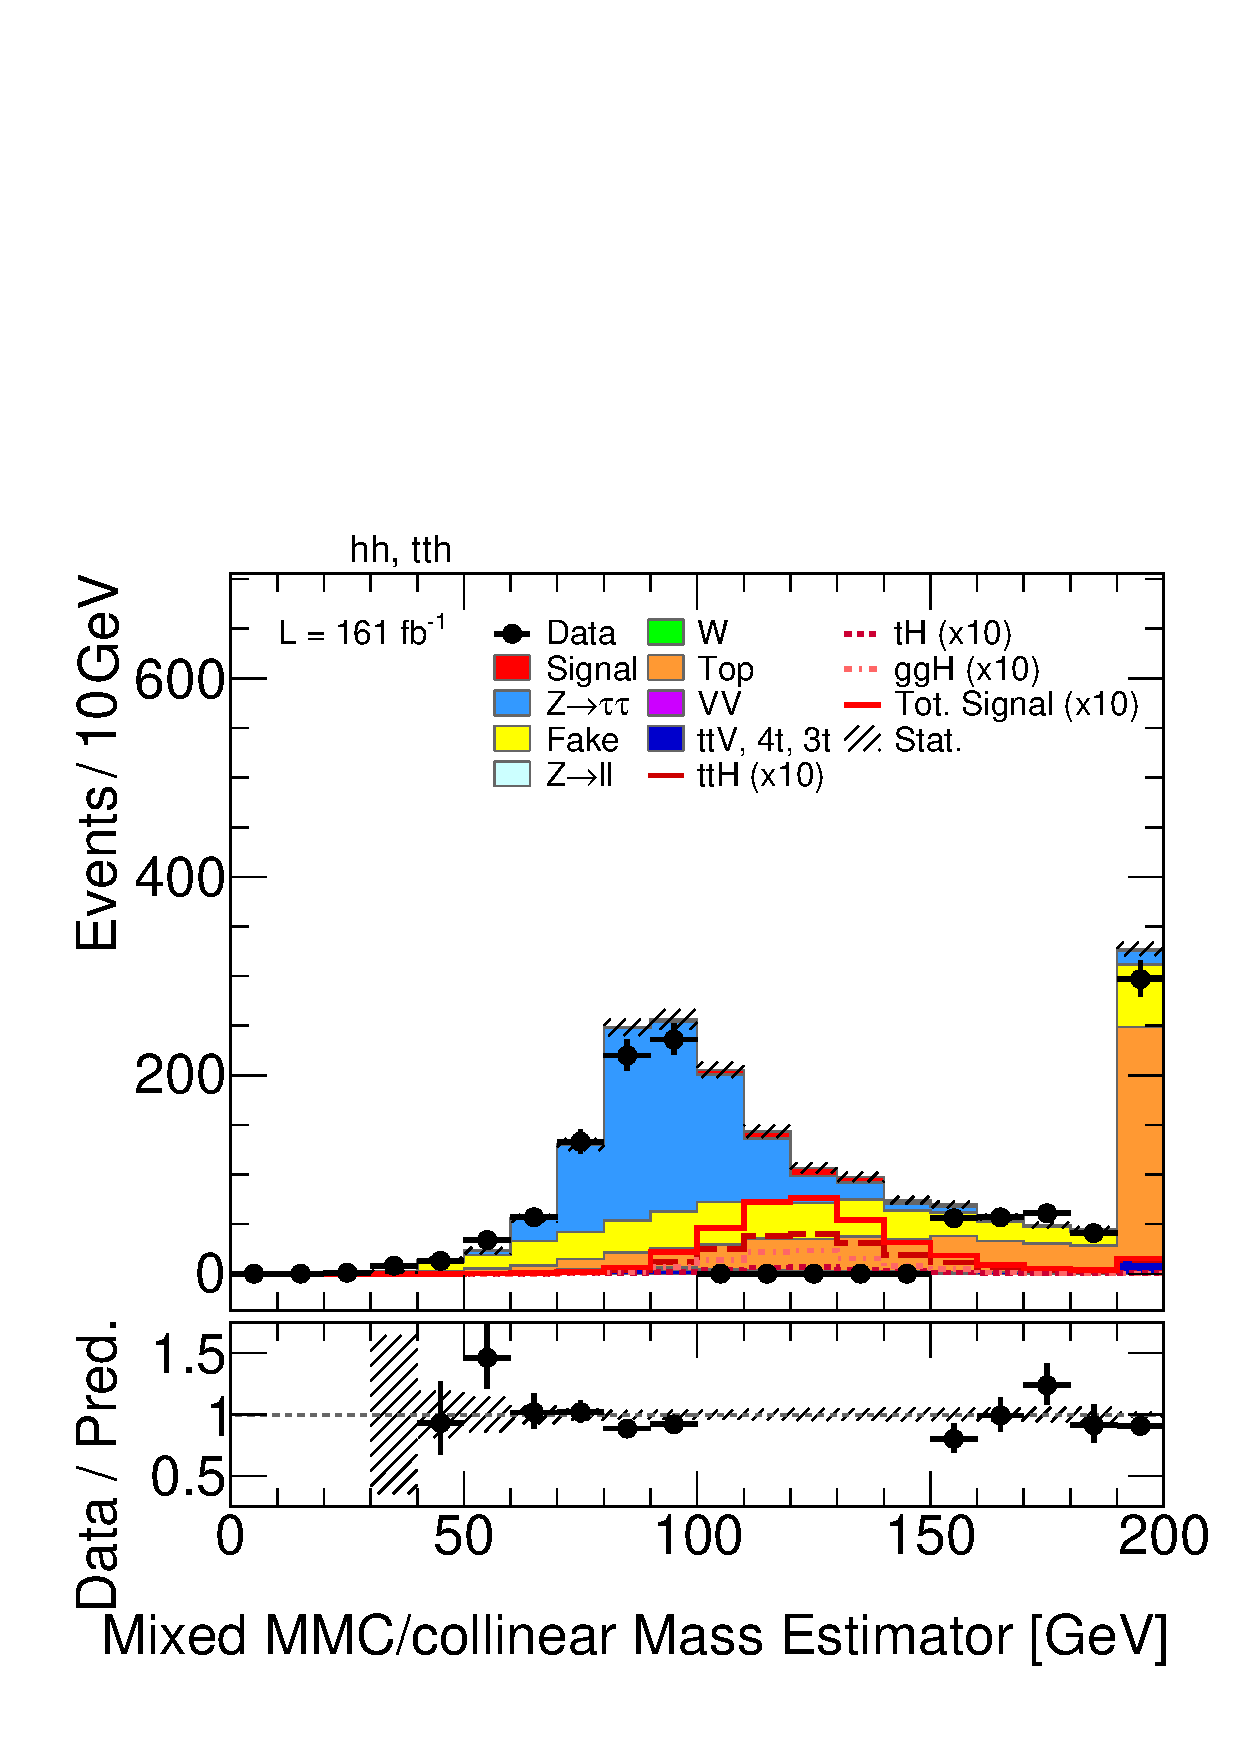
\includegraphics[width=\textwidth]{scaled_plot_ditau_mmc_mlm_m_fix_hh_tth_22_23_24.pdf}
      \caption{}
    \end{subfigure}
    \caption{
      Distribution of \mmc at preselection level in Run-3. 
      The comparison between data and MC is shown (a) without applying the global rescaling and (b) after rescaling the \ttbar and \ztautau MC samples by factors of 1.2 and 1.4, respectively.
    }
    \label{mmc_scaled}
  \end{figure}
  
The following sections describe in detail the key aspects of the new analysis: updated object reconstruction techniques and phase space definitions, revisited MVA methods incorporating the $tHqb$ signal, the estimation of fake-$\tau$ backgrounds, and finally the new event categorisation and statistical fit strategy.


\section{Events and object definition}

In this new analysis there are no major updates regarding the trigger requirements used to select events of interest. For the reconstruction of physics objects, which form the basis of both the event selection and categorisation, we follow the same techniques and procedures as previously described in Section~\ref{subsec:object_def} and Chapter~\ref{chap:object_rec}. Electrons, muons, hadronically decaying $\tau$-leptons, jets, and missing transverse momentum are reconstructed and identified according to the standard ATLAS prescriptions.

A key difference with respect to the Run-2 analysis presented in Chapter~\ref{chap:htautau} is that the present study uses data reprocessed with \textsc{Athena} release 22. This introduces several improvements in object identification that are particularly relevant for this analysis. The most important ones concern the identification of hadronically decaying $\tau$-leptons and the flavour tagging of jets initiated by $b$-quarks. In the case of $b$-tagging, the algorithm used in release 21 has been replaced in release 22 by \textsc{gn2v01}, a graph-based neural network employing a Transformer architecture to predict jet flavour. The model takes as inputs individual track parameters, their uncertainties, and the jet kinematics ($p_{\mathrm{T}}$ and $\eta$). Two auxiliary tasks are included during training: the first predicts track-pair vertex compatibility, i.e.\ whether two tracks originate from a common spatial point, which removes the need for a dedicated secondary-vertex algorithm, while the second assigns each track to an underlying physics process, distinguishing whether it originates from a $b$-hadron, a $c$-hadron, a light-flavour quark, pile-up, or is a fake track. In this analysis the working point corresponding to a 70\% $b$-jet tagging efficiency is employed, providing a good balance between signal acceptance and background rejection. Jets are required to have $p_{\mathrm{T}}>20$~GeV and $|\eta|<2.5$.

For hadronic $\tau$-lepton identification, the RNN-based method used during Run-2 (trained separately for 1-prong and 3-prong decays) has been replaced by a new algorithm referred to as \textsc{gnTau}. Following the same philosophy as for the new $b$-tagging approach, this method relies on a graph neural network infrastructure with similar inputs, and provides improved discrimination of \tauhadvis candidates from quark- and gluon-initiated jets. As discussed in Section~\ref{fakes_run3}, this new algorithm significantly reduces the contribution from fake-$\tau$ backgrounds, which represented an important source of contamination in the previous analysis due to the large jet multiplicities required.

The preselection for the $tH$ and $t\bar{t}H$ analyses largely follows that defined in the previous study and summarised in Table~\ref{tab:tth_hadhad_selection}, with the updates described above. In particular, the jet requirements are relaxed: at least five jets are required in the final state, of which at least one must be $b$-tagged at the 70\% working point. This configuration provides the most efficient balance between signal acceptance and background contamination for both $tHqb$ and $t\bar{t}H$. Although requiring only four jets with at least one $b$-tag would increase acceptance for $tHqb$, the gain would be offset by a substantial increase in the $t\bar{t}$ background, as illustrated in Figure~\ref{jets_selection}. 
\begin{figure}[htbp]
    \centering
    \begin{subfigure}[b]{0.45\textwidth}
      \centering
      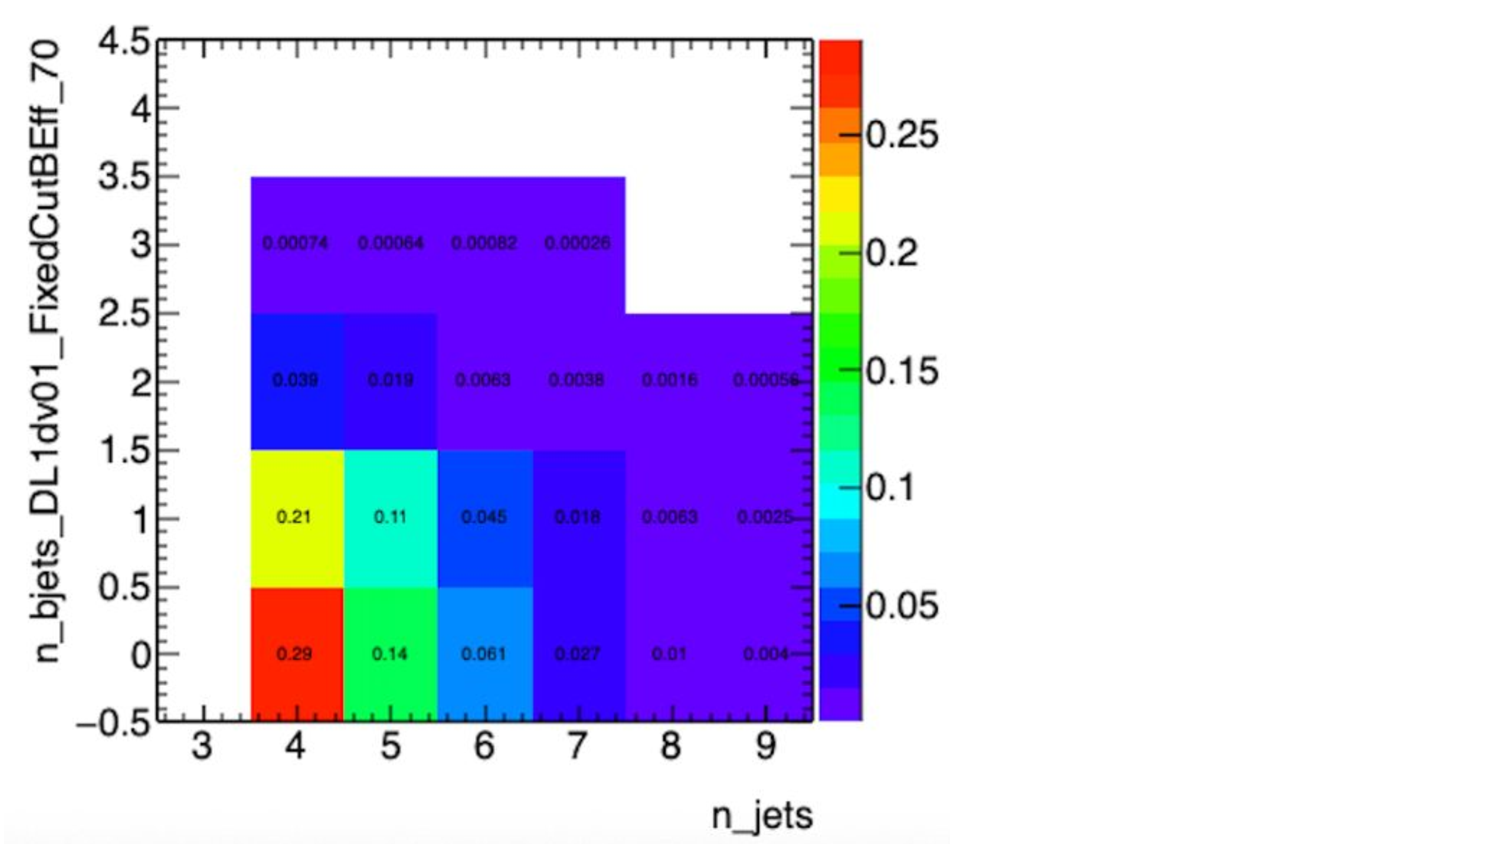
\includegraphics[width=\textwidth]{jets_selection/Ztt}
      \caption{}
      \label{fig:jetsel_ztt}
    \end{subfigure}
    \hfill
    \begin{subfigure}[b]{0.45\textwidth}
      \centering
      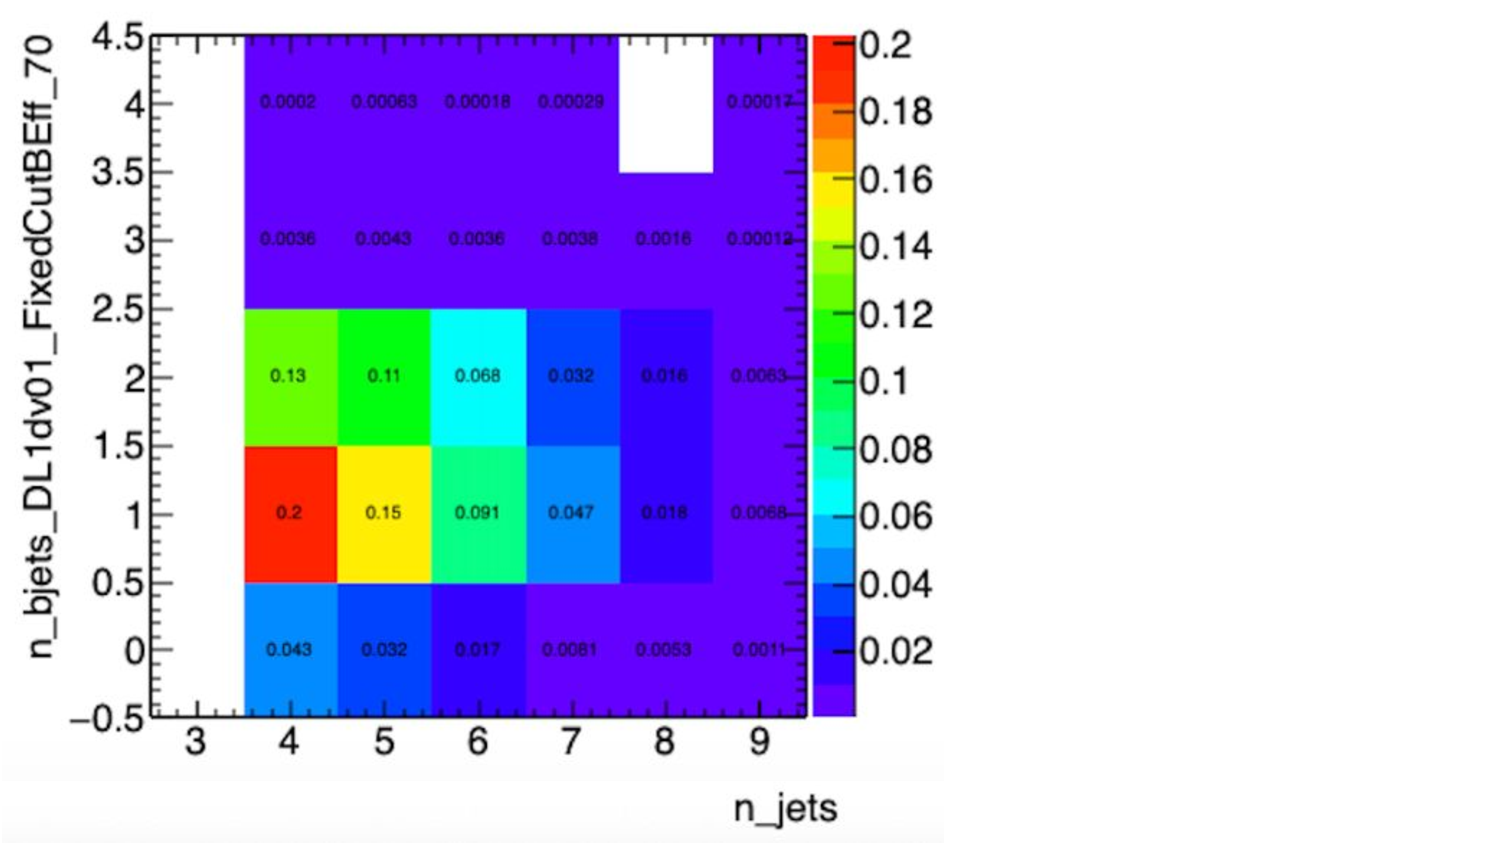
\includegraphics[width=\textwidth]{jets_selection/ttbar}
      \caption{}
      \label{fig:jetsel_ttbar}
    \end{subfigure}
    \\[0.3cm]
    \begin{subfigure}[b]{0.45\textwidth}
      \centering
      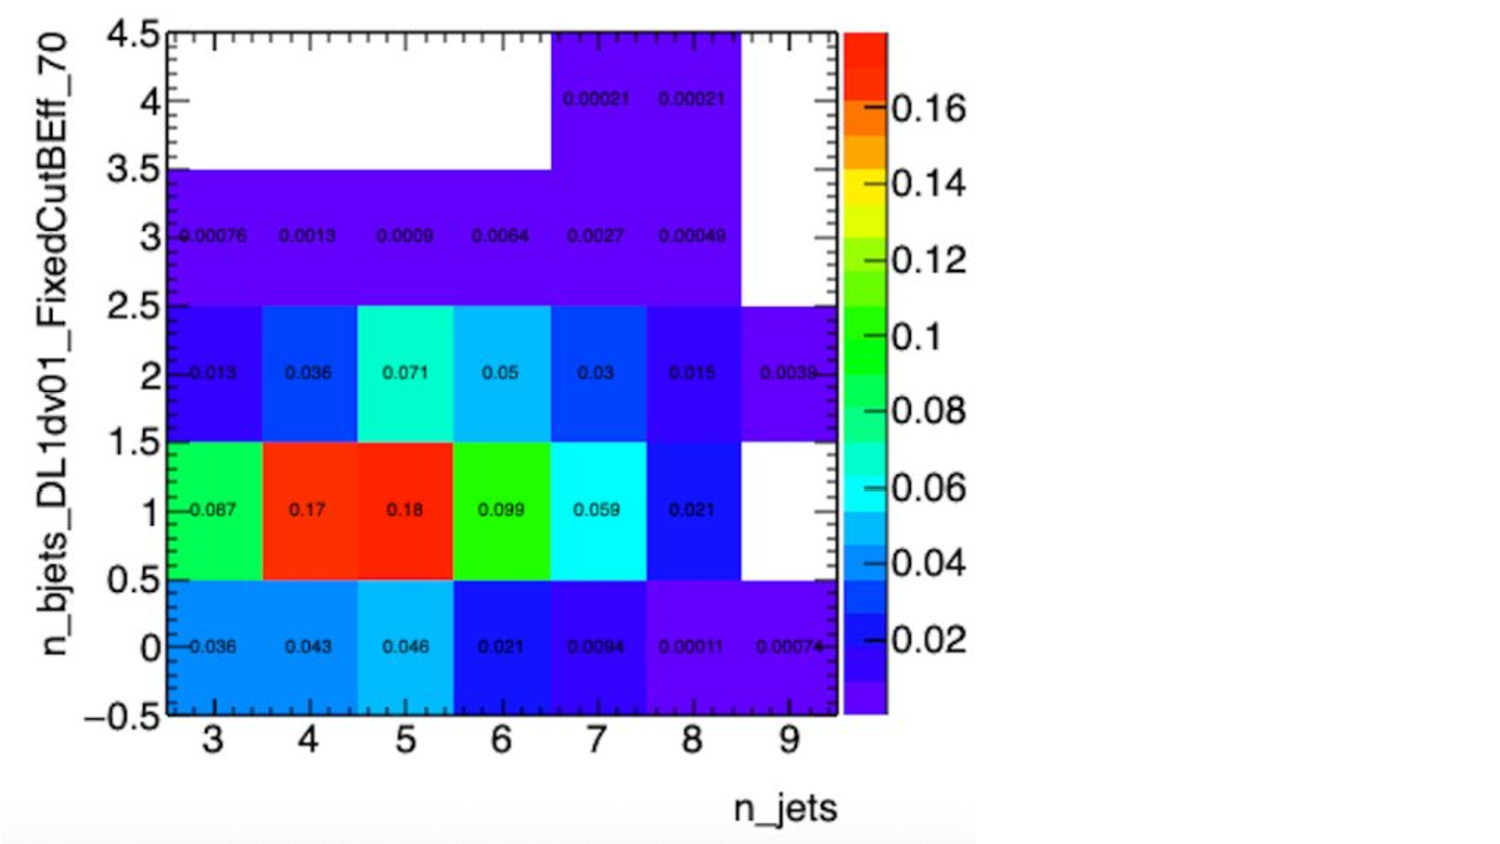
\includegraphics[width=\textwidth]{jets_selection/tH}
      \caption{}
      \label{fig:jetsel_th}
    \end{subfigure}
    \hfill
    \begin{subfigure}[b]{0.45\textwidth}
      \centering
      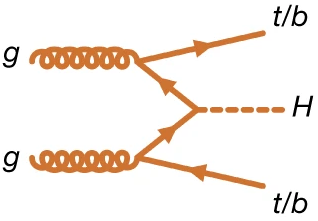
\includegraphics[width=\textwidth]{jets_selection/ttH}
      \caption{}
      \label{fig:jetsel_tth}
    \end{subfigure}
    \caption{
      Fraction of events passing different requirements on the jet and $b$-jet multiplicities
      for the main signal and background processes. 
      The heatmaps show the fraction of selected events for (a) $Z\to\tau\tau$, (b) $t\bar{t}$, (c) $tHqb$, and (d) $t\bar{t}H$, 
      as a function of the number of reconstructed jets and the number of $b$-tagged jets.
    }
    \label{jets_selection}
  \end{figure}
  
It is also important to highlight that, for process discrimination, the topology of $tHqb$ exhibits a distinctive feature: the spectator jet from the hard scatter tends to be very forward, as it carries a large fraction of the longitudinal momentum of the initial-state valence quark. This provides a clear signature of $tHqb$, which is absent in $t\bar{t}H$, where the leading jets originate from the two top quarks and therefore populate the more central region of the detector, as shown in Figure~\ref{fig:feynman_tH_ttH}.
\begin{figure}[htbp]
    \centering
    \begin{subfigure}[b]{0.37\textwidth}
      \centering
      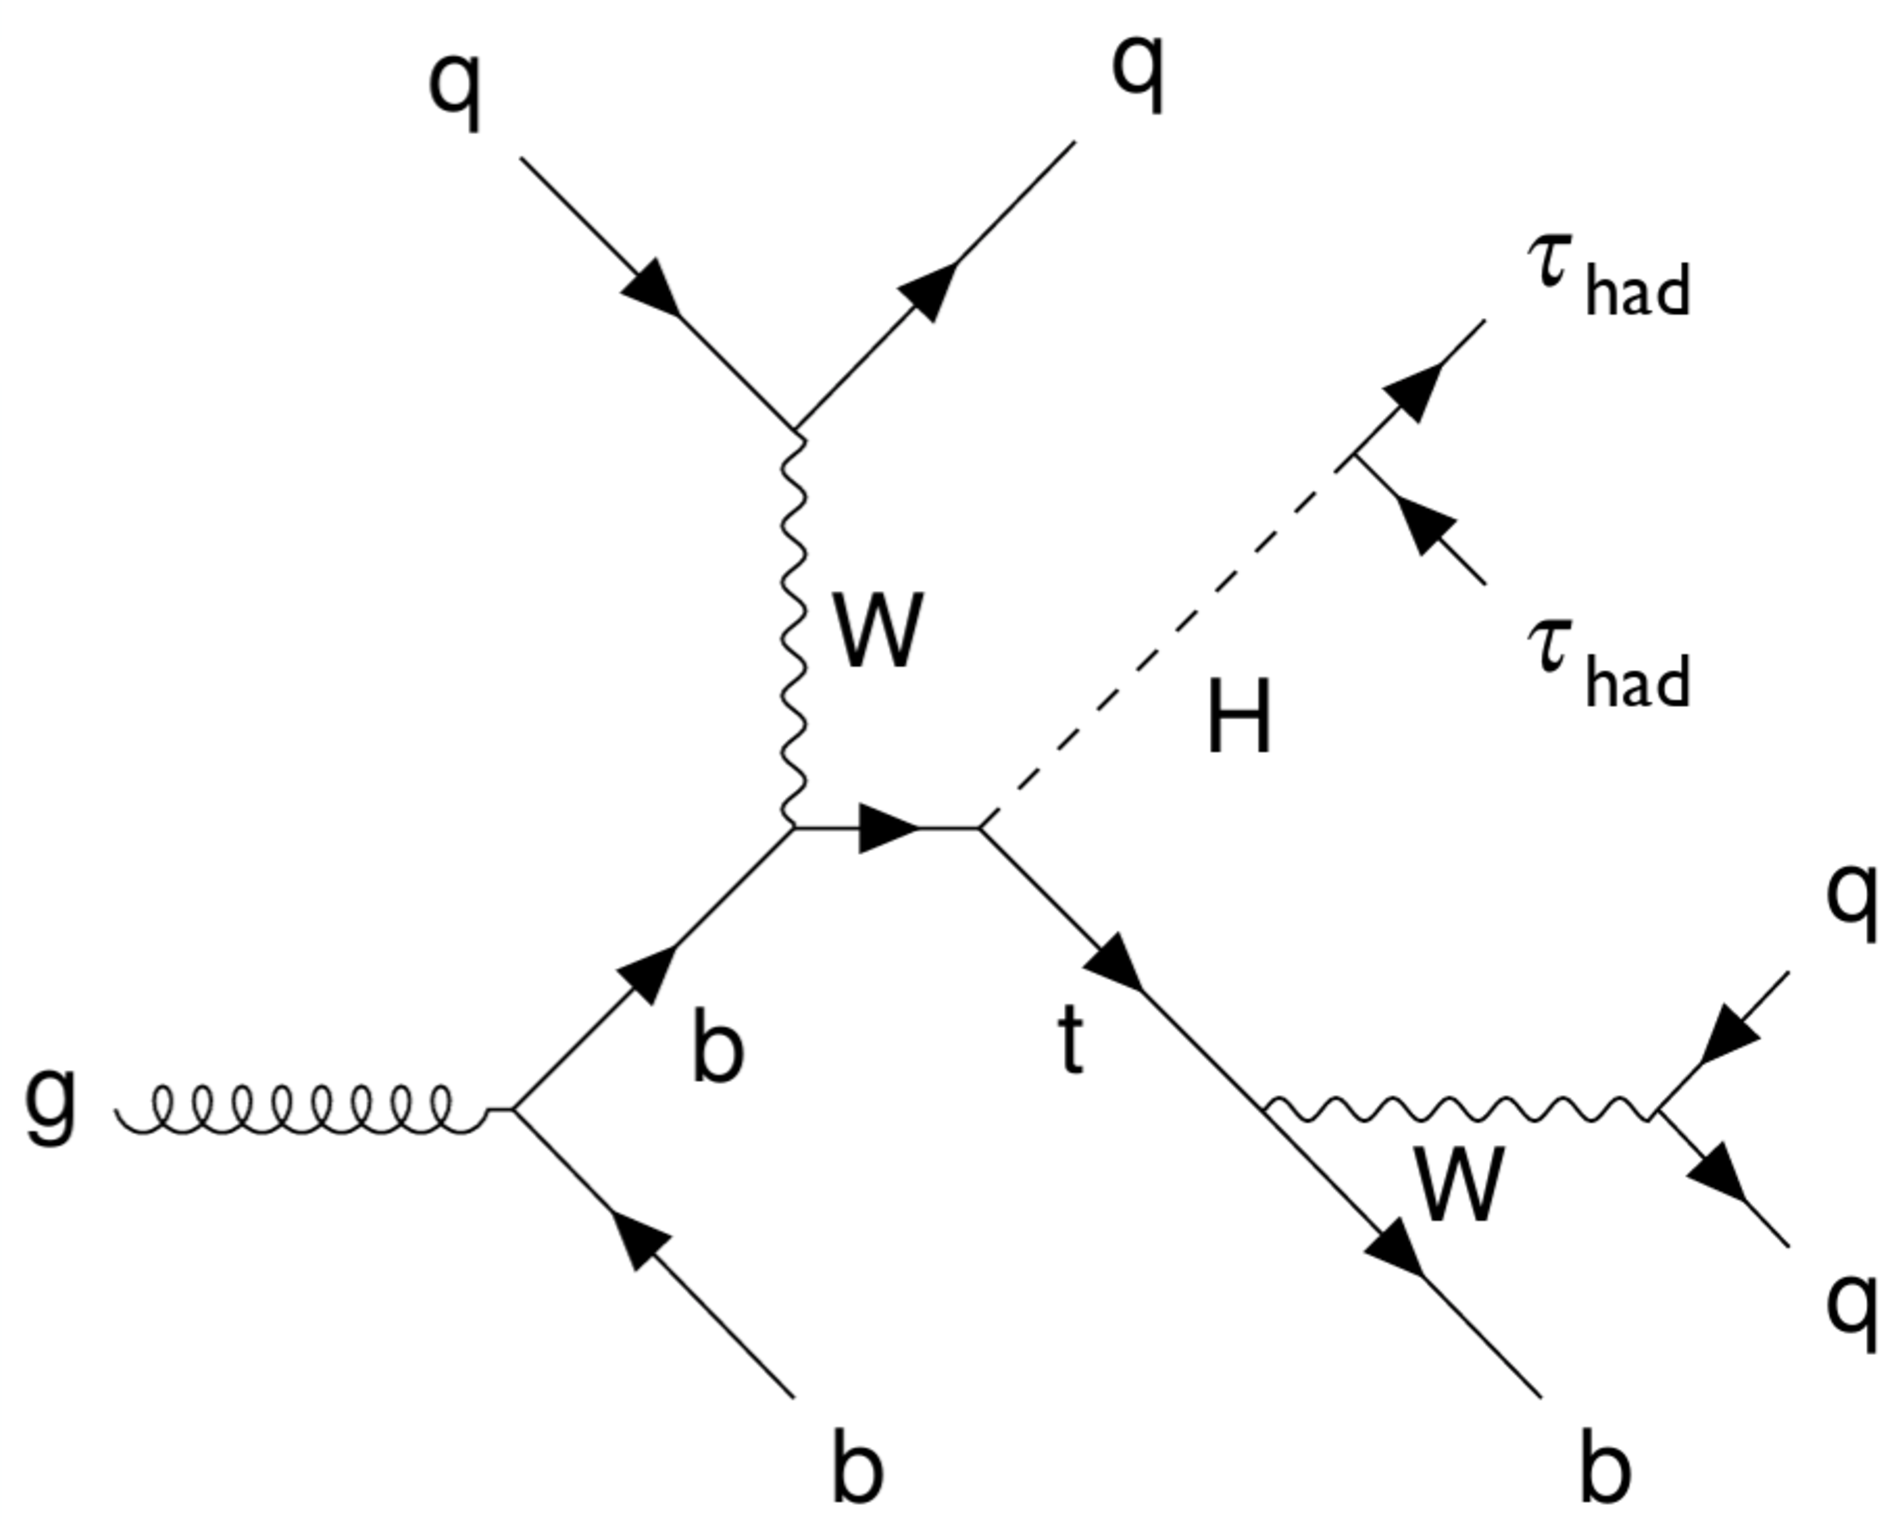
\includegraphics[width=\textwidth]{thqbtautau.pdf}
      \caption{}
    \end{subfigure}
    \begin{subfigure}[b]{0.4\textwidth}
      \centering
      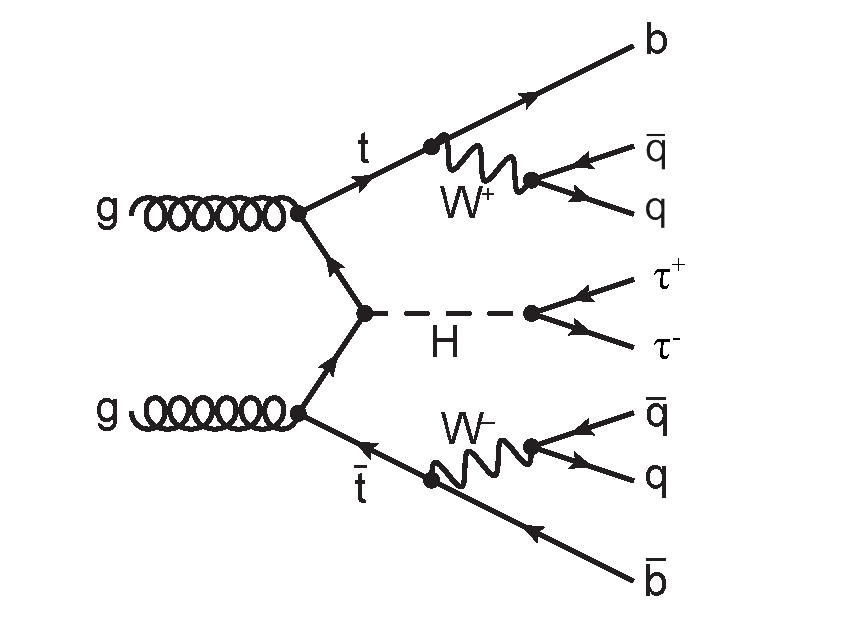
\includegraphics[width=\textwidth]{tth_diagram_1}
      \caption{}
    \end{subfigure}
    \caption{Representative leading-order Feynman diagrams for (a) $tH(\tau\tau)qb$ in the $t$-channel~\cite{Barger_2010} and (b) \ttHtt.}
    \label{fig:feynman_tH_ttH}
  \end{figure}



\section{Fakes background estimation}
\label{fakes_run3}

In the previous analysis it was noted that, when estimating the contribution from fake backgrounds, the dedicated control regions were derived by inverting the identification criteria applied to the $\tau$-lepton candidates in the signal regions. From these control regions, templates enriched in fake objects were obtained and subsequently used both to derive the fake factors (FFs) and to apply them in the analysis signal regions. An important detail was that one could not simply invert the Medium working point: at least one of the $\tau_{\mathrm{had}}$ candidates still had to satisfy a loose identification requirement, since events without any loosely identified $\tau_{\mathrm{had}}$ were not considered in the analysis. This limitation is no longer present in the samples processed with release 22, which simplifies the estimation procedure in the current study.

In the present analysis, the fake background is re-estimated by defining a single control region in which the $\tau_{\mathrm{had}}$ candidates fail the Medium working point, without imposing any additional Loose requirement. A single set of fake factors, $FF_{nm}$ following Eq.~\ref{eq_fakes}, is therefore enough to describe the background contribution. 

The fake factors are derived in bins of \pt and $|\eta|$ of the $\tau$-lepton, using dedicated \taulephad control regions. Separate determinations are performed depending on whether the hadronic $\tau$-lepton decay is classified as 1-prong or 3-prong. Distinct sets of fake factors are also derived and subsequently applied for the Run-2 and Run-3 datasets. Figure~\ref{fig:ff_run2_run3} shows the resulting fake factors for both data-taking periods, displayed as a function of \pt in the two $|\eta|$ regions considered: the ``Barrel'' region ($0<|\eta|<1.37$) and the ``Endcap'' region, which covers the remaining acceptance.
\begin{figure}[htbp]
    \centering
    \begin{subfigure}[b]{0.49\textwidth}
      \centering
      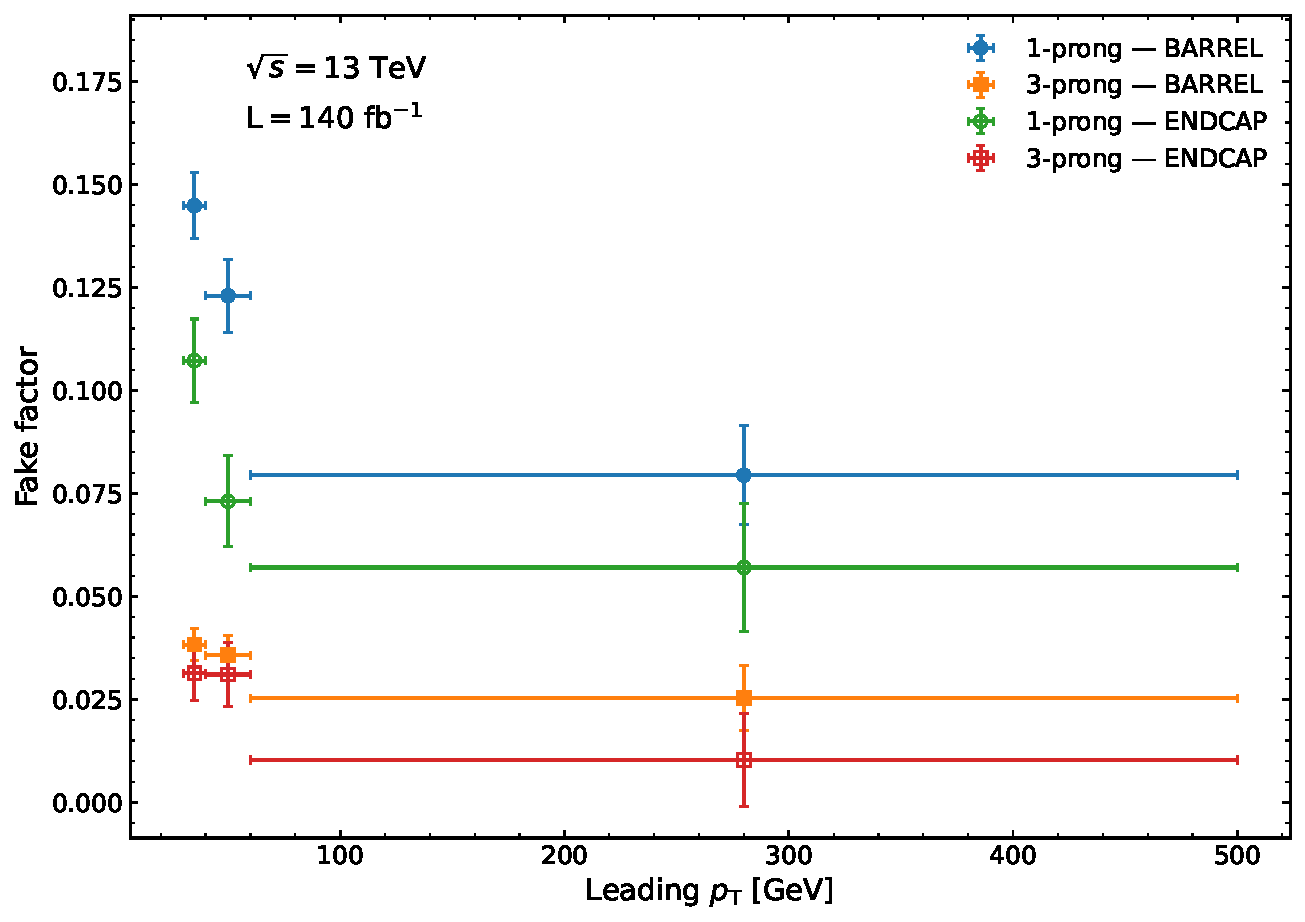
\includegraphics[width=\textwidth]{new_FFs_trigger_corrected_ATLAS_run2.pdf}
      \caption{}
      \label{fig:ff_run2}
    \end{subfigure}
    \hfill
    \begin{subfigure}[b]{0.49\textwidth}
      \centering
      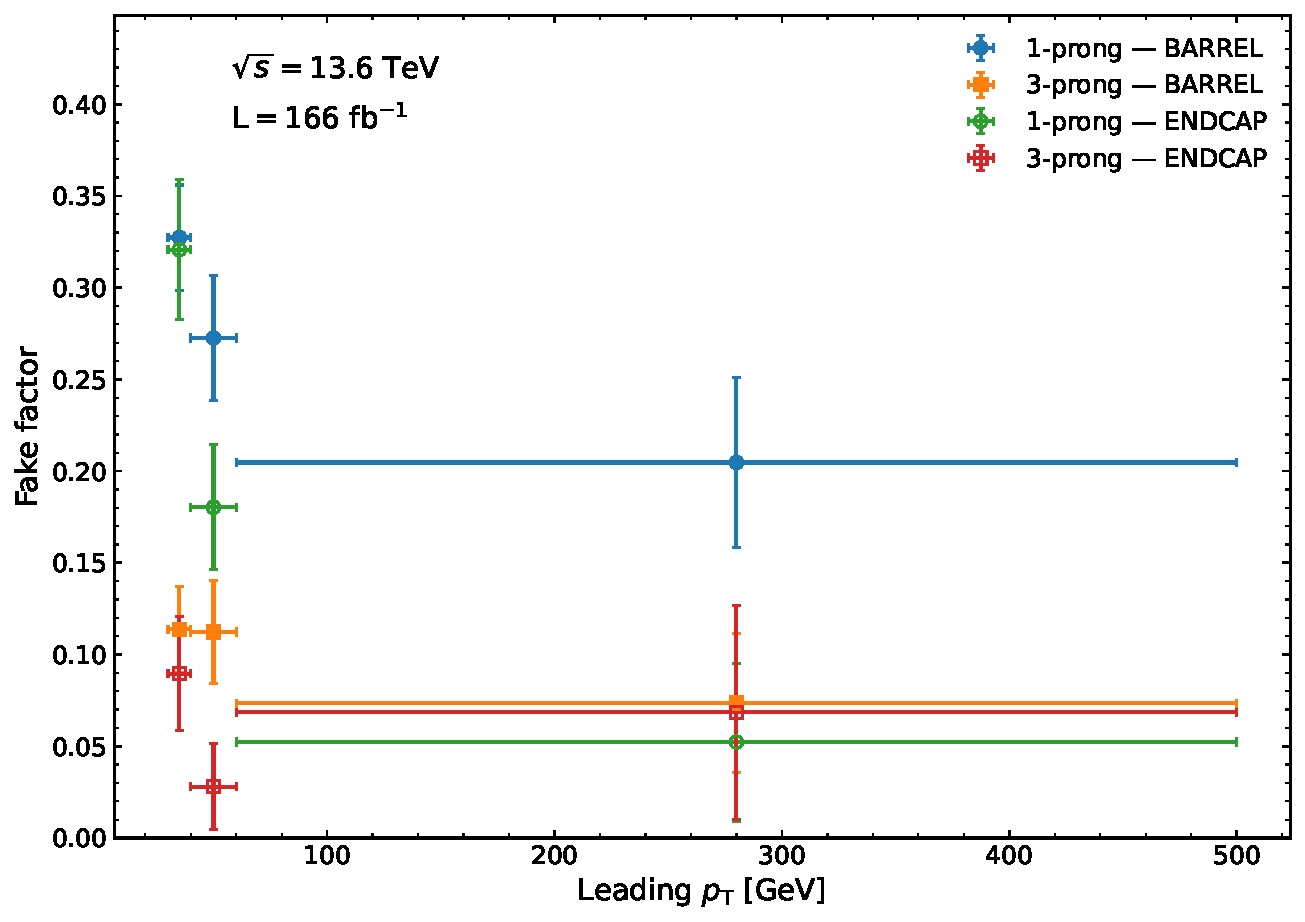
\includegraphics[width=\textwidth]{new_FFs_trigger_corrected_ATLAS_run3.pdf}
      \caption{}
      \label{fig:ff_run3}
    \end{subfigure}
    \caption{
      Fake factors in the \tauhadhad channel as a function of the leading $p_{\mathrm{T}}$,
      shown separately for BARREL and ENDCAP and for 1-prong and 3-prong candidates.
      Panels (a) and (b) correspond to Run-2
      and Run-3, respectively.
    }
    \label{fig:ff_run2_run3}
  \end{figure}
From these plots it can be concluded that the fake factors required to scale the background from misidentified \tauhad are significantly larger for Run-3 data compared to Run-2, particularly at low \pt, with the effect being especially pronounced in the 1-prong category. More importantly, however, the new fake factors derived with release~22 Run-2 samples using the updated \textsc{gntau} identification algorithm are noticeably smaller than those obtained in the previous round of the analysis presented in the preceding chapter, which relied on the RNN-based approach for \tauhad identification~\cite{serhat_tesis}, as illustrated in Figure~\ref{fig:ffs_run2_rnn}.  
  \begin{figure}[htbp]
    \centering
    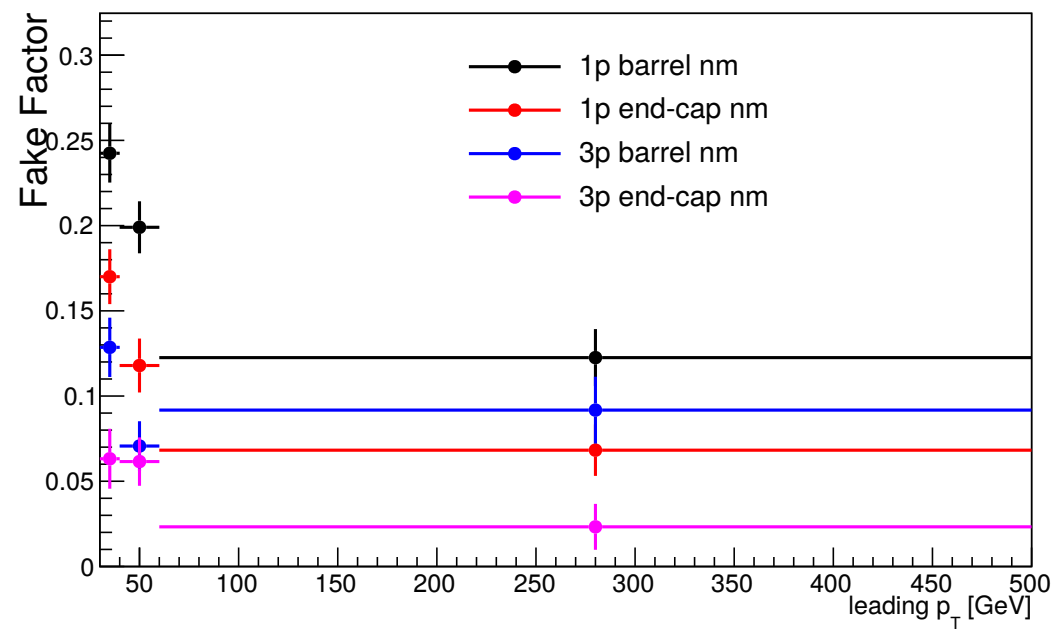
\includegraphics[width=0.55\textwidth]{ffs_run2_legacy}
    \caption{Fake factors derived in Run-2 using the RNN-based \tauhad identification, 
    shown as a function of the $\tau$-lepton transverse momentum for the same two $|\eta|$ regions considered: Barrel and Endcap~\cite{serhat_tesis}.}
    \label{fig:ffs_run2_rnn}
  \end{figure}
This difference is observed across all \pt and $|\eta|$ bins, as well as as a function of the prongness. At first sight, it could suggest that the new \textsc{gntau} algorithm achieves a better performance in rejecting jets faking \tauhad. In practice, however, this effect originates primarily from the way the templates are constructed when defining the anti-ID regions in the two approaches. In the following, the closure or validation of this new fake background estimate is presented, together with a comparison to the results obtained in the previous round, in order to quantify the extent to which this background has been reduced.

In this simplified scenario, the application of the FFs follows a straightforward event-by-event reweighting: events in which only one $\tau_{\mathrm{had}}$ candidate fails the Medium ID are scaled by $FF_{nm}$ of the failing $\tau$, while events where both candidates fail are scaled by the product of the two fake factors. The full prediction in the signal region is thus given by
\begin{align}
    \tau_1^{P}\,\tau_2^{P} \;=\;&\;
    \tau_1^{T}\,\tau_2^{T}\;(\text{MC}) \nonumber \\[0.2cm]
    &+\, FF_{nm}(\tau_1)\;\tau_1^{F}\,\tau_2^{P} \nonumber \\[0.2cm]
    &+\, FF_{nm}(\tau_2)\;\tau_1^{P}\,\tau_2^{F} \nonumber \\[0.2cm]
    &-\, FF_{nm}(\tau_1)\,FF_{nm}(\tau_2)\;\tau_1^{F}\,\tau_2^{F}\,,
    \label{eq_fakes}
    \end{align}
where $P$ and $F$ denote whether a $\tau_{\mathrm{had}}$ candidate passes or fails the Medium ID, respectively, and $\tau^T$ refers to genuine $\tau$-leptons taken from simulation.  
To validate the estimation of this background contribution, the distributions of representative observables such as the transverse momentum and pseudorapidity of the leading and subleading \tauhad candidates are shown at preselection level, but inclusive in jet multiplicity to allow for a clearer visualization.  
These plots are evaluated in a same-sign region, which is enriched in events with misidentified \tauhad candidates. In these events, the large jet multiplicity and the random charge assignment of tracks increase the probability of jets mimicking the signature of hadronic $\tau$ decays. Good agreement between data and the background estimation is expected. 
    
  \begin{figure}[htbp]
    \centering
    \begin{subfigure}[b]{0.45\textwidth}
      \centering
      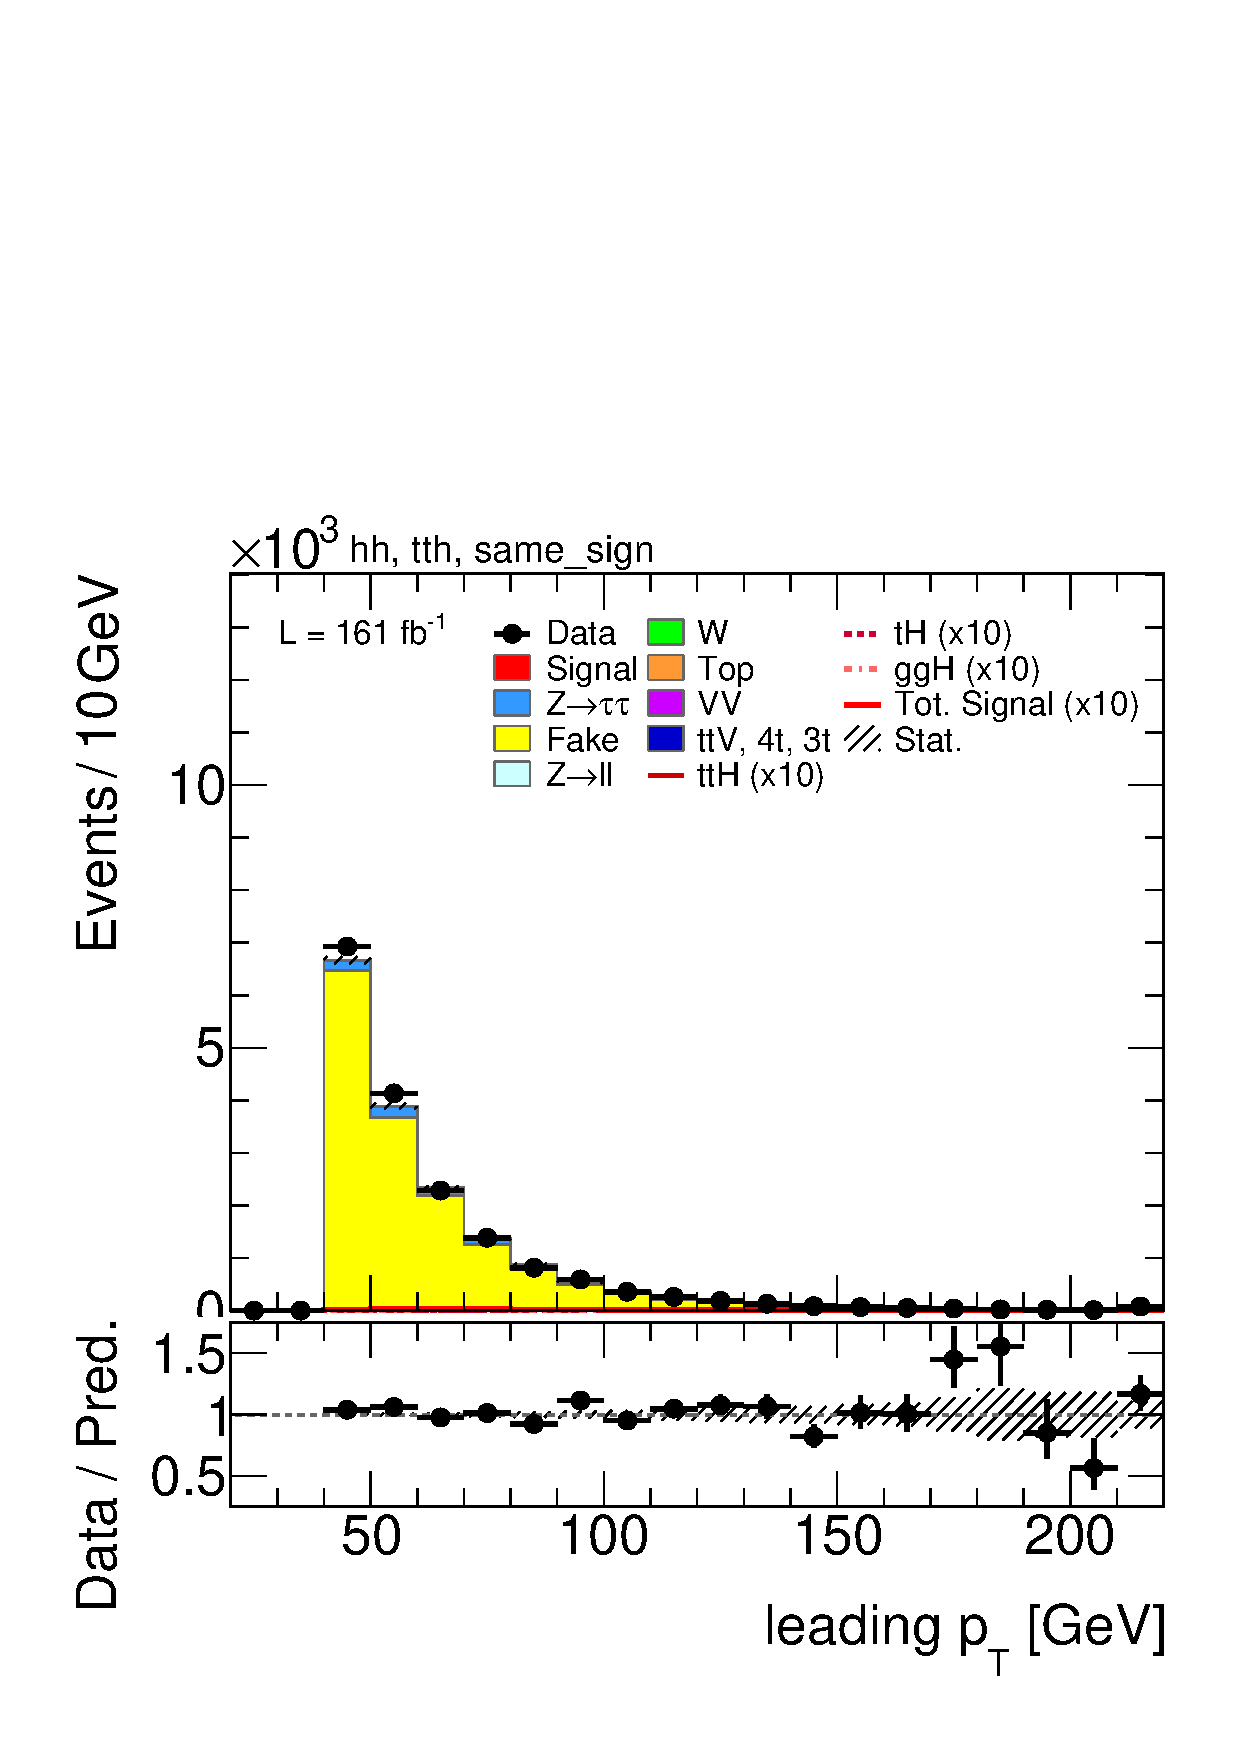
\includegraphics[width=\textwidth]{images/fakes_run3/plot_tau_0_pt_hh_tth_22_23_24_same_sign.pdf}
      \caption{}
    \end{subfigure}
    \hfill
    \begin{subfigure}[b]{0.45\textwidth}
      \centering
      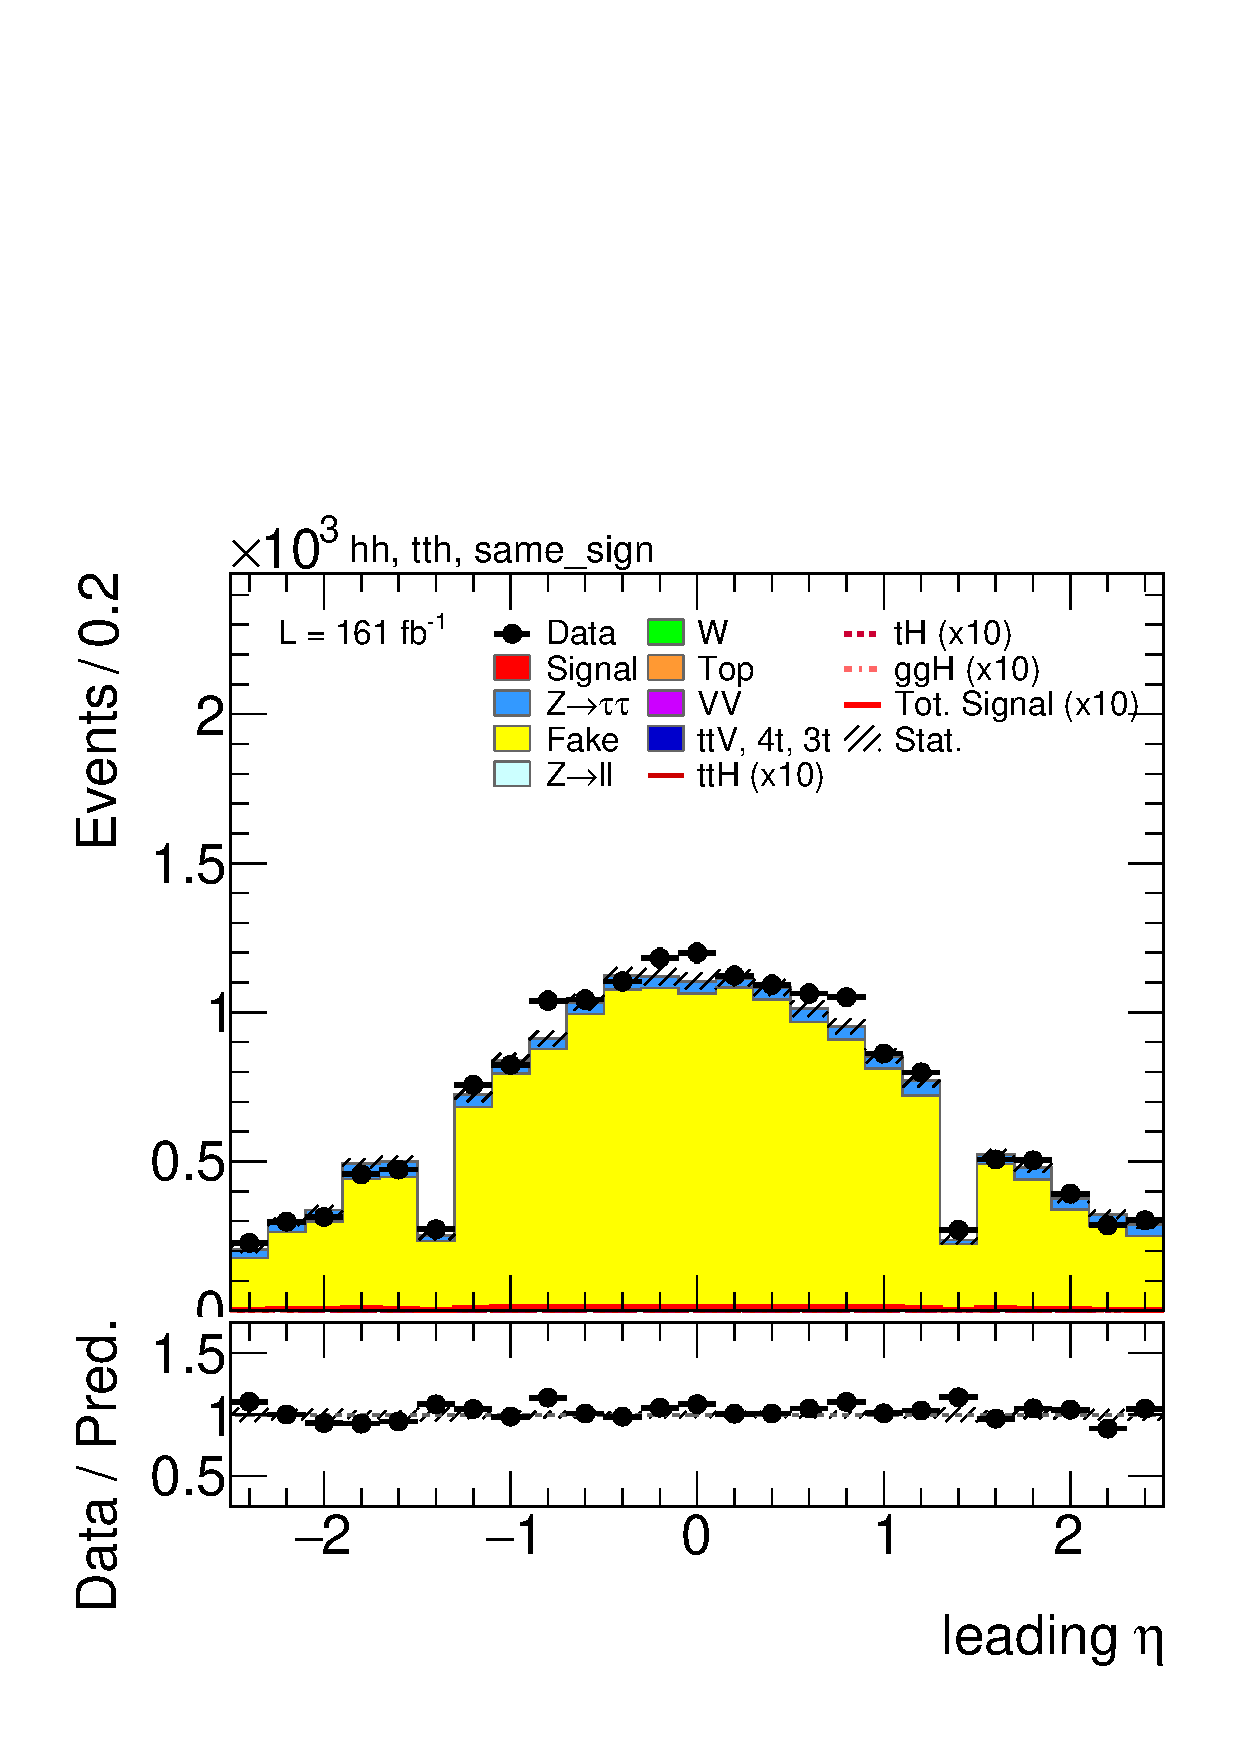
\includegraphics[width=\textwidth]{images/fakes_run3/plot_tau_0_eta_hh_tth_22_23_24_same_sign.pdf}
      \caption{}
    \end{subfigure}

    \begin{subfigure}[b]{0.45\textwidth}
      \centering
      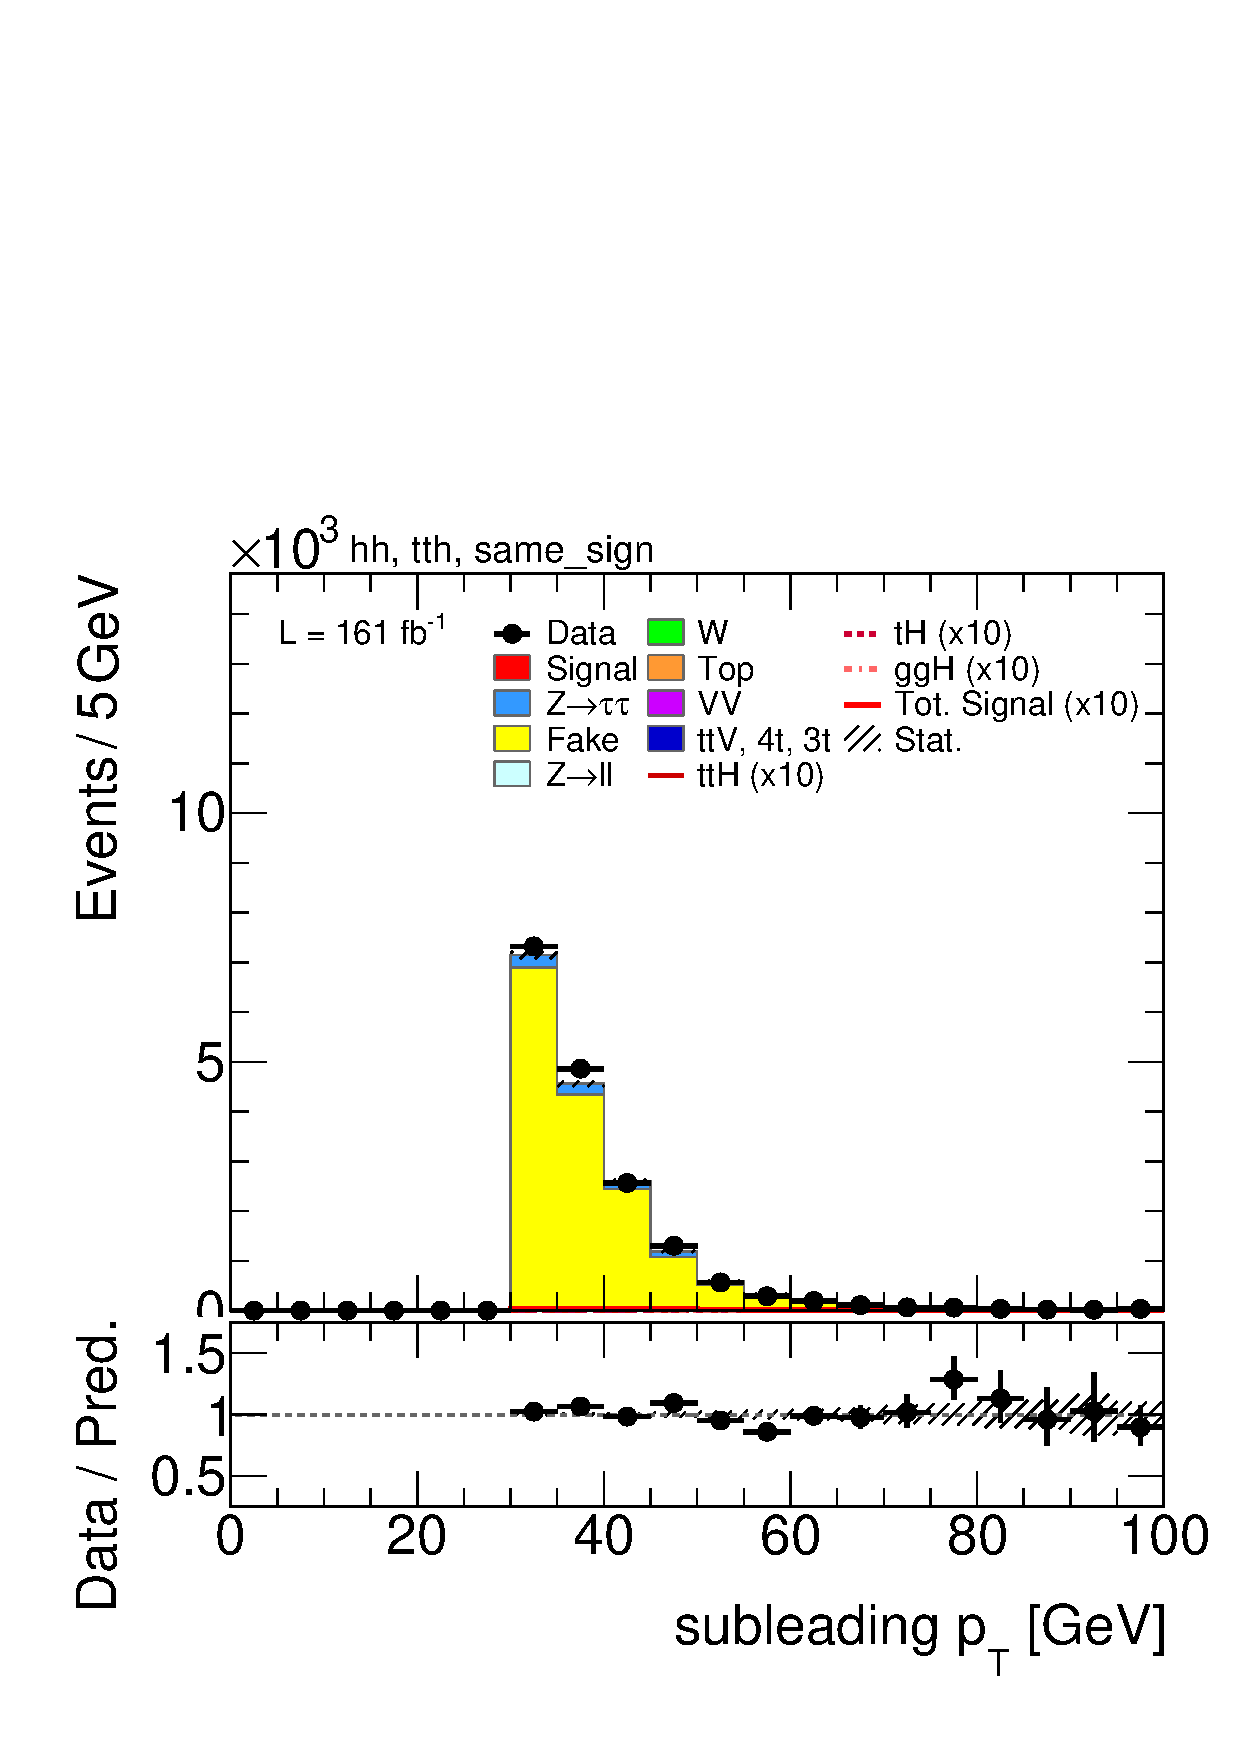
\includegraphics[width=\textwidth]{images/fakes_run3/plot_tau_1_pt_hh_tth_22_23_24_same_sign.pdf}
      \caption{}
    \end{subfigure}
    \hfill
    \begin{subfigure}[b]{0.45\textwidth}
      \centering
      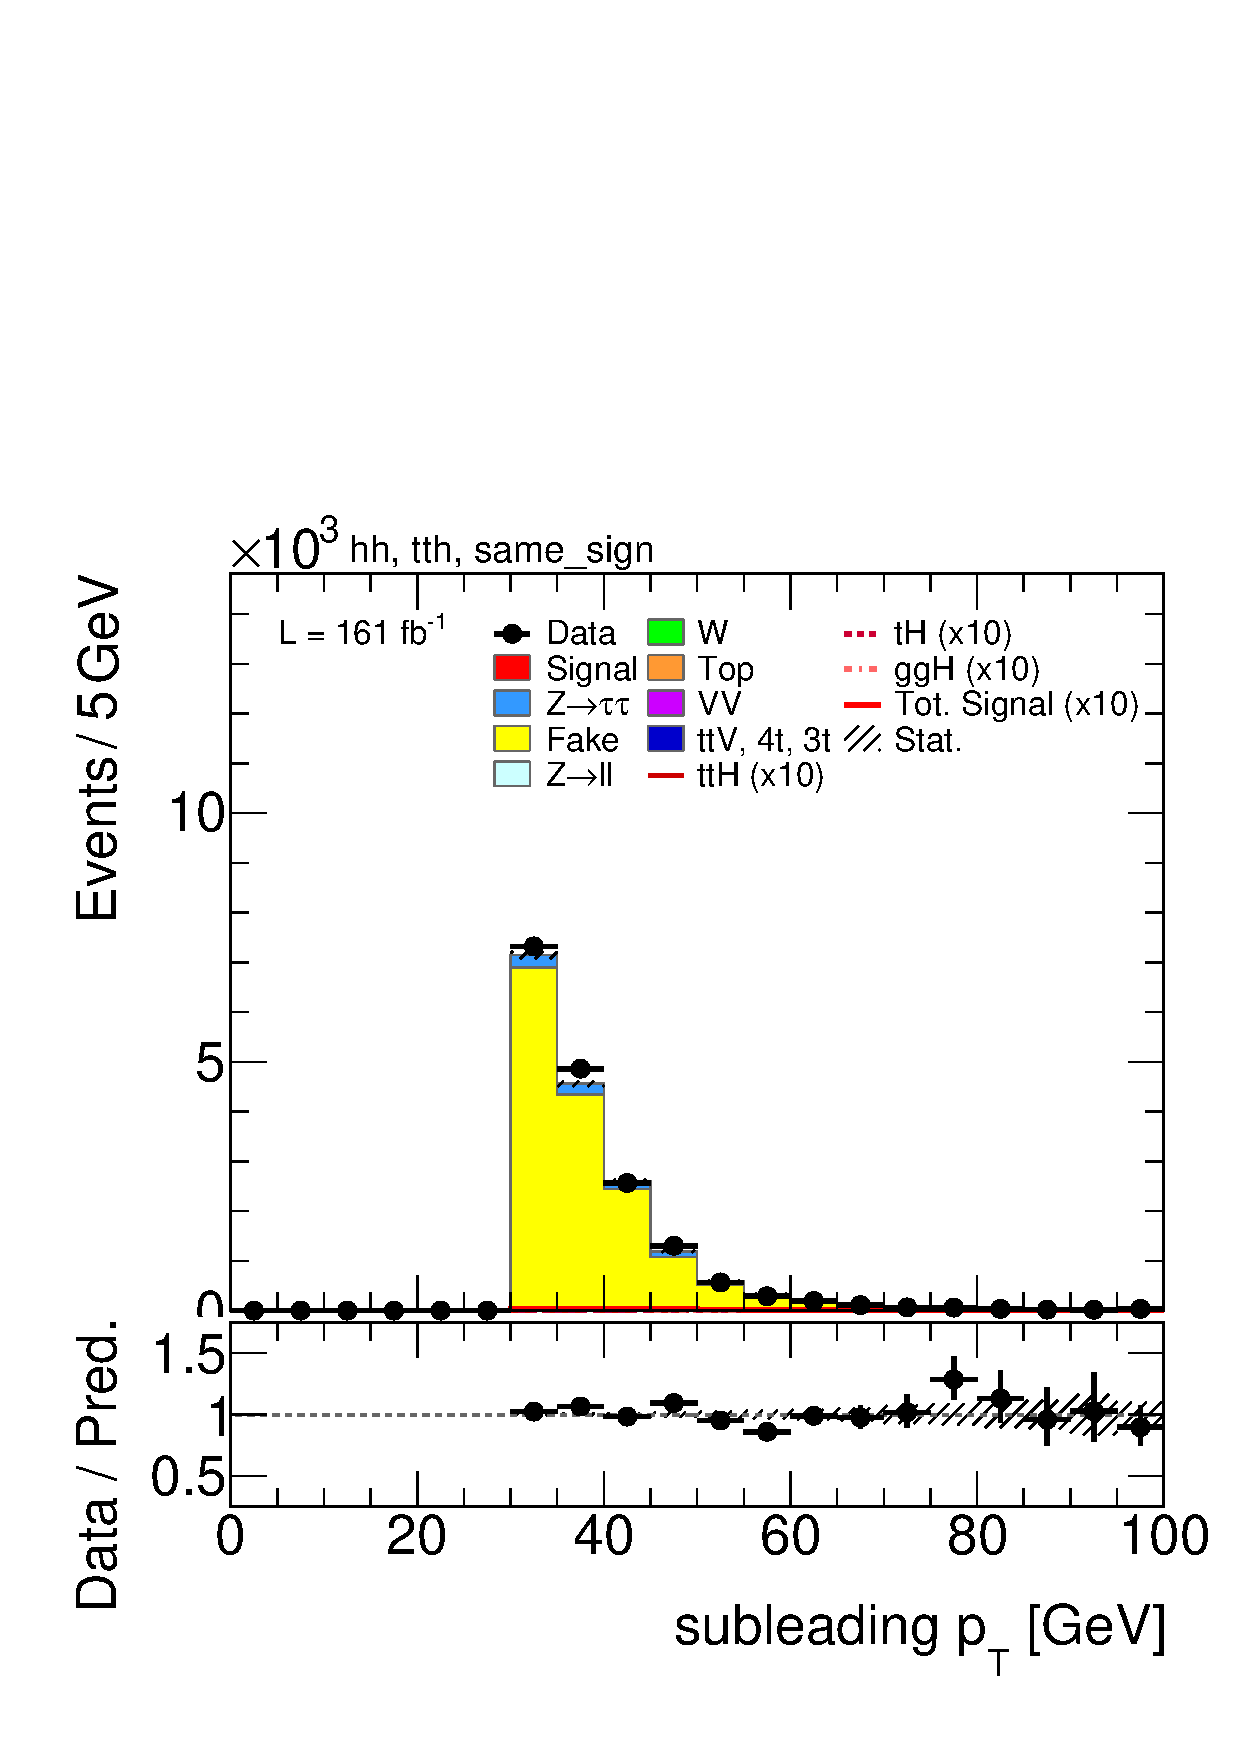
\includegraphics[width=\textwidth]{images/fakes_run3/plot_tau_1_pt_hh_tth_22_23_24_same_sign.pdf}
      \caption{}
    \end{subfigure}
  
    \caption{
      Closure and validation of the fake background estimation in Run-3 dataset, evaluated in the same-sign region at preselection level.
      The comparison is shown as a function of the \pt and $\eta$ of the leading (a), (b), and subleading (c), (d), \tauhad candidates. 
      Data are compared to the estimated fake background. Scaling factors on \ztautau and \ttbar are applied.
    }
    \label{fig:closure_validation_run3}
  \end{figure}

  \begin{figure}[htbp]
    \centering
    \begin{subfigure}[b]{0.45\textwidth}
      \centering
      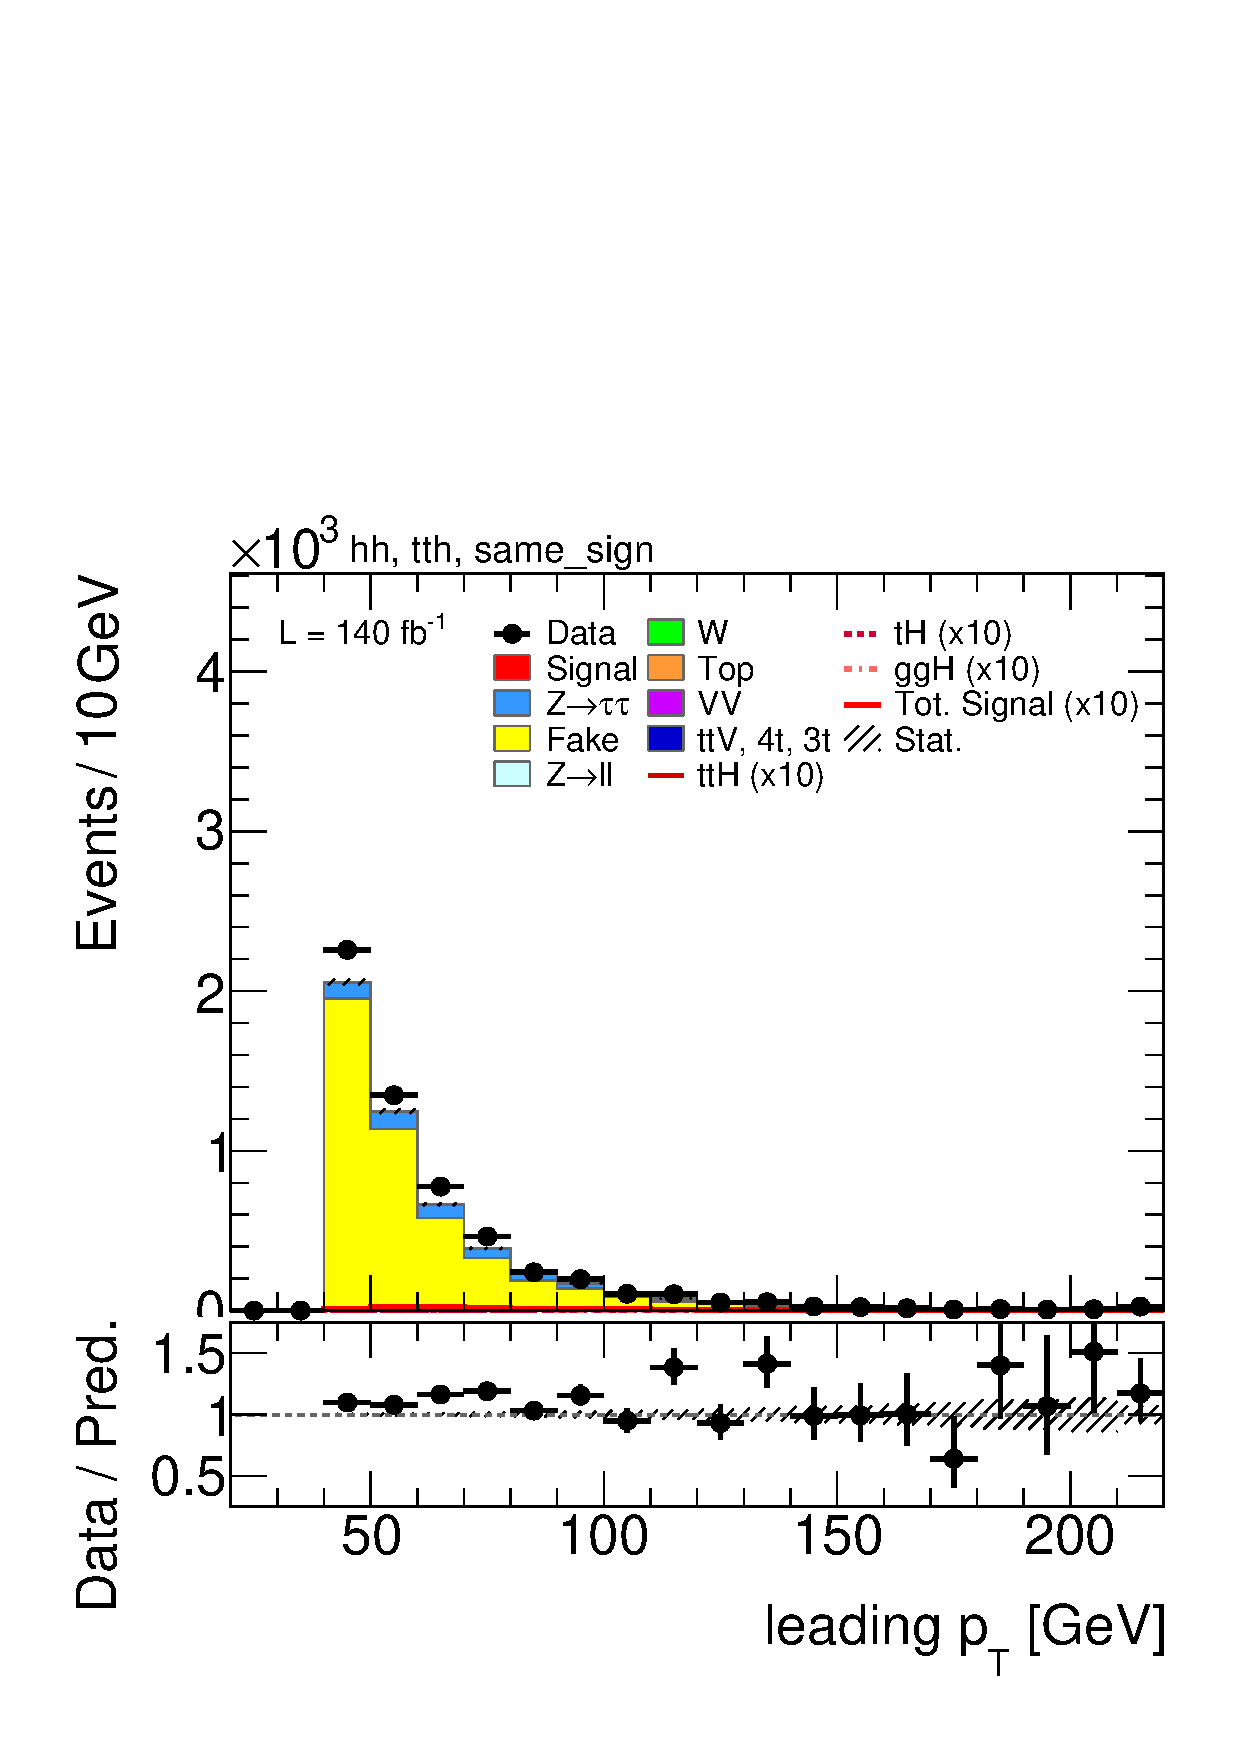
\includegraphics[width=\textwidth]{images/fakes_run2/plot_tau_0_pt_hh_tth_15_16_17_18_same_sign.pdf}
      \caption{}
    \end{subfigure}
    \hfill
    \begin{subfigure}[b]{0.45\textwidth}
      \centering
      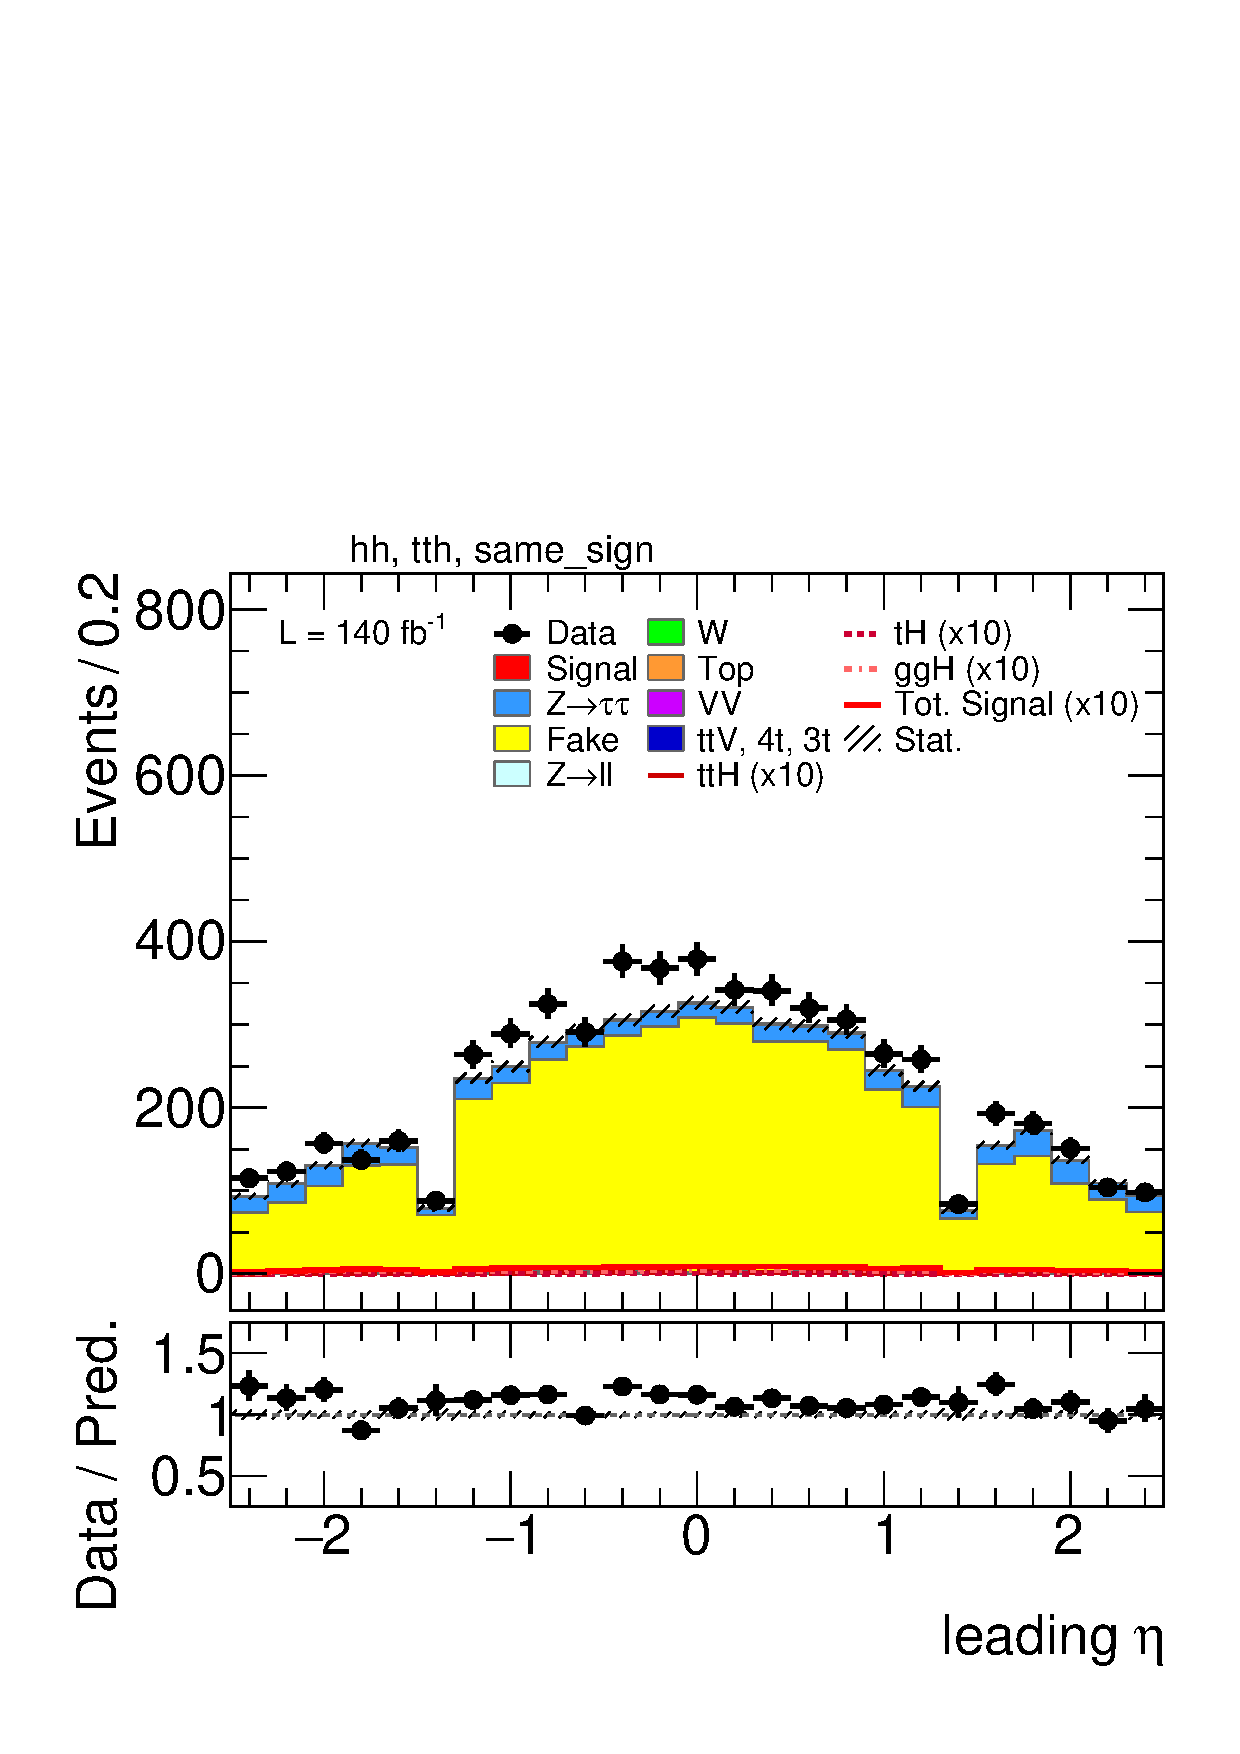
\includegraphics[width=\textwidth]{images/fakes_run2/plot_tau_0_eta_hh_tth_15_16_17_18_same_sign.pdf}
      \caption{}
    \end{subfigure}

    \begin{subfigure}[b]{0.45\textwidth}
      \centering
      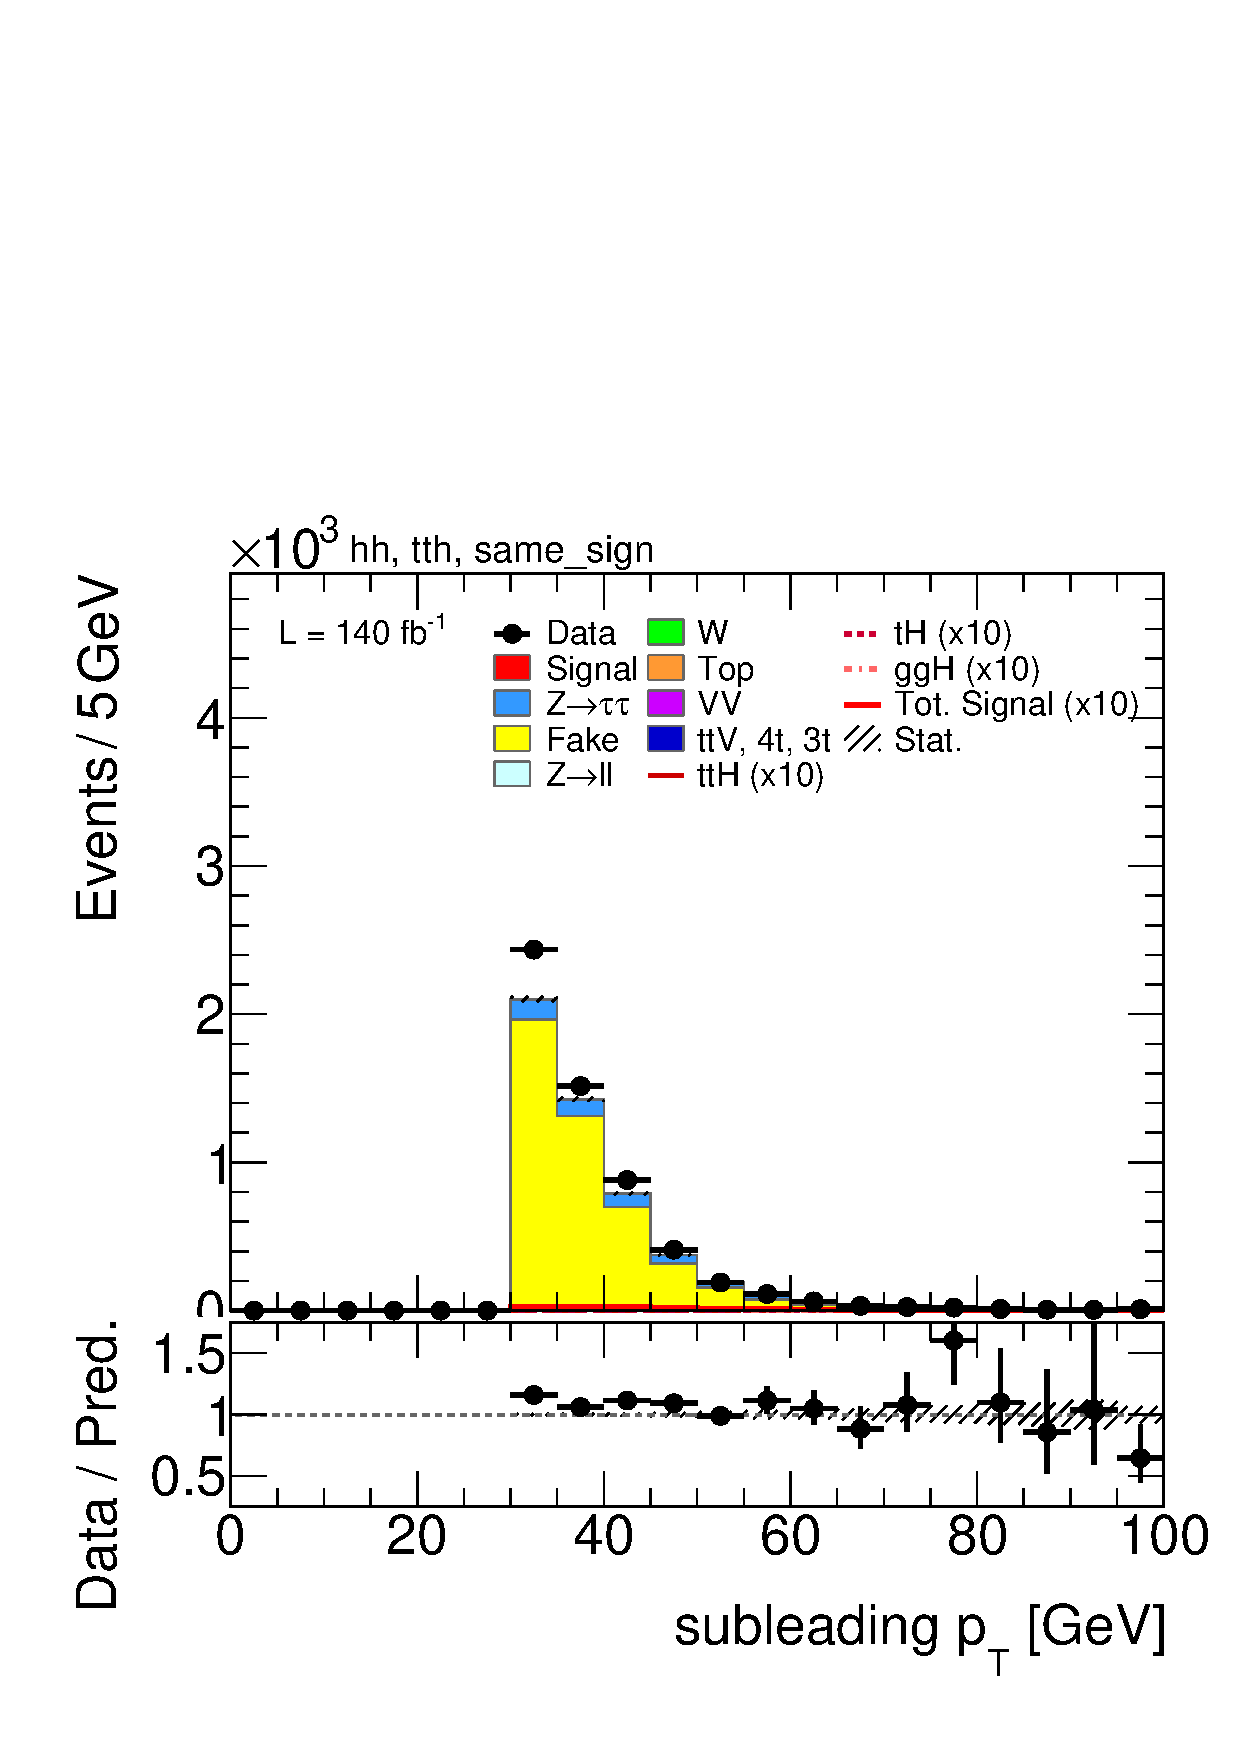
\includegraphics[width=\textwidth]{images/fakes_run2/plot_tau_1_pt_hh_tth_15_16_17_18_same_sign.pdf}
      \caption{}
    \end{subfigure}
    \hfill
    \begin{subfigure}[b]{0.45\textwidth}
      \centering
      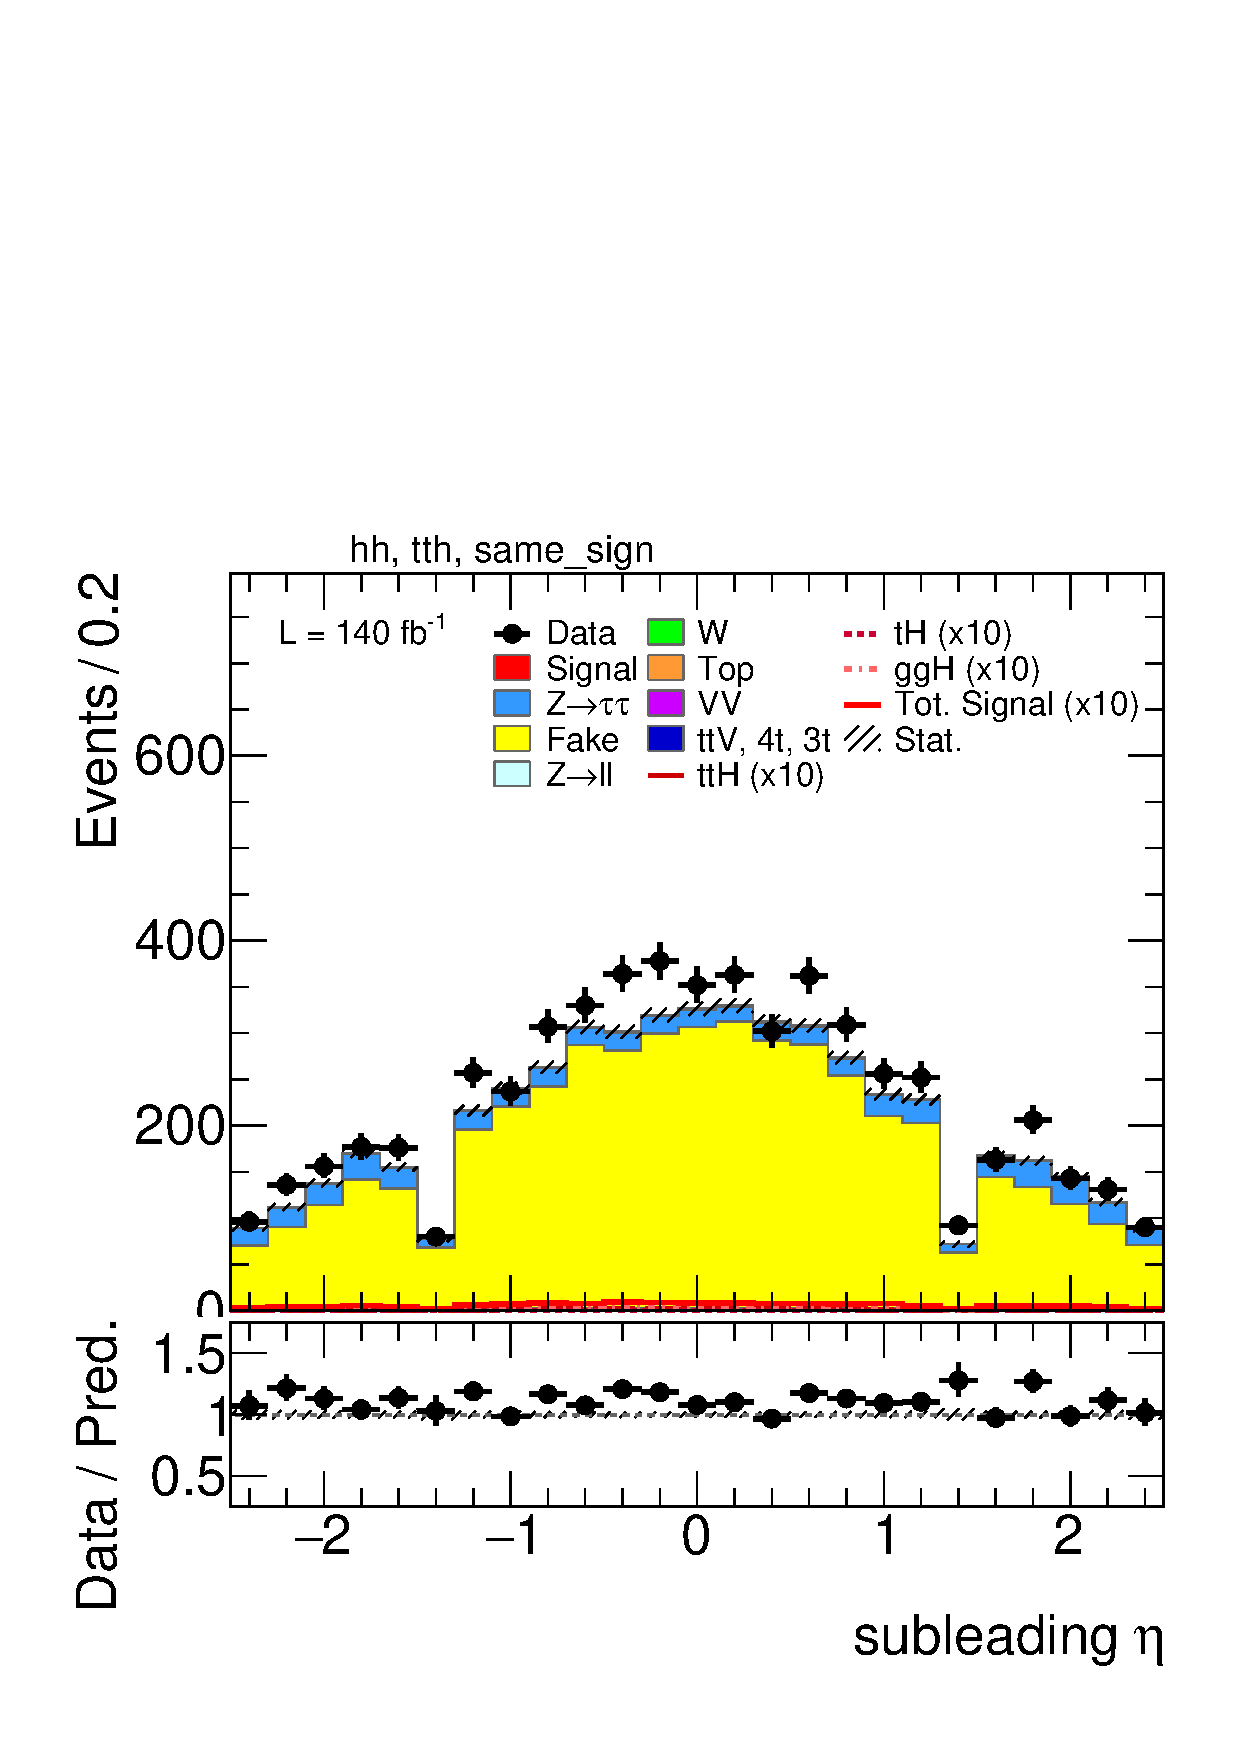
\includegraphics[width=\textwidth]{images/fakes_run2/plot_tau_1_eta_hh_tth_15_16_17_18_same_sign.pdf}
      \caption{}
    \end{subfigure}
  
    \caption{
      Closure and validation of the fake background estimation in Run-2 dataset, evaluated in the same-sign region at preselection level.
      The comparison is shown as a function of the \pt and $\eta$ of the leading (a), (b), and subleading (c), (d), \tauhad candidates. 
      Data are compared to the estimated fake background.
    }
    \label{fig:closure_validation_run2}
  \end{figure}

  In Figure~\ref{run2_fakes_comparison}, the effect of switching from the RNN-based to the new \textsc{gntau} identification algorithm is illustrated using a dataset corresponding to 2022 data-taking period.  
  The distributions of the jet multiplicity, as well as the transverse momentum and pseudorapidity of the leading \tauhad candidate, are shown for the \ttH preselection requiring at least one $b$-tagged jet.  
  This choice provides a more inclusive selection, ensuring sufficient statistical precision to clearly illustrate the effect, while the requirement of at least one $b$-tagged jet enhances the visibility of the \ttbar contribution, yielding a representative picture of the phase space relevant for the analysis.  
  A marked reduction in the contribution from misidentified \tauhad backgrounds is observed when employing the \textsc{gntau} algorithm, highlighting its superior performance in suppressing jets misidentified as hadronic $\tau$ decays, with overall reductions of about 60-70\% compared to the previous RNN-based approach.
  
  \begin{figure}[htbp]
    \centering
    % Top row: GNTau
    \begin{subfigure}[b]{0.45\textwidth}
        \centering
        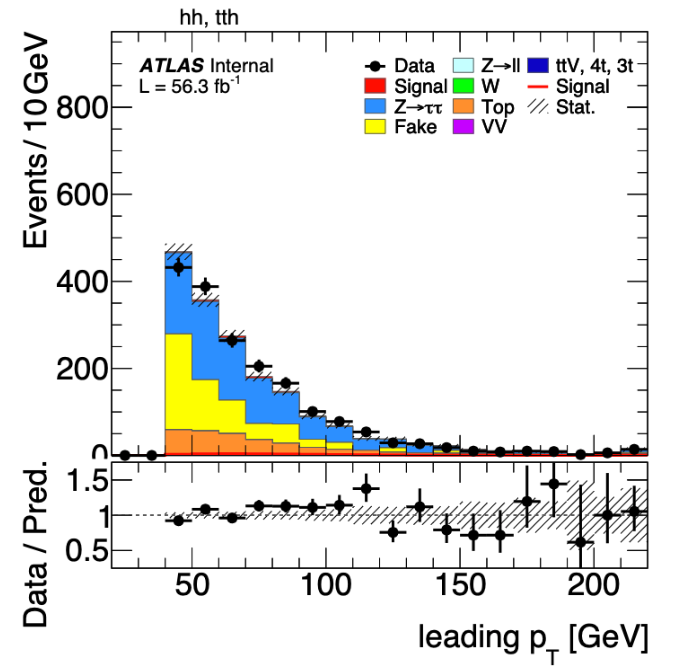
\includegraphics[width=\textwidth]{images/leading_pt_gntau.png}
        \caption{}
    \end{subfigure}
    \begin{subfigure}[b]{0.45\textwidth}
        \centering
        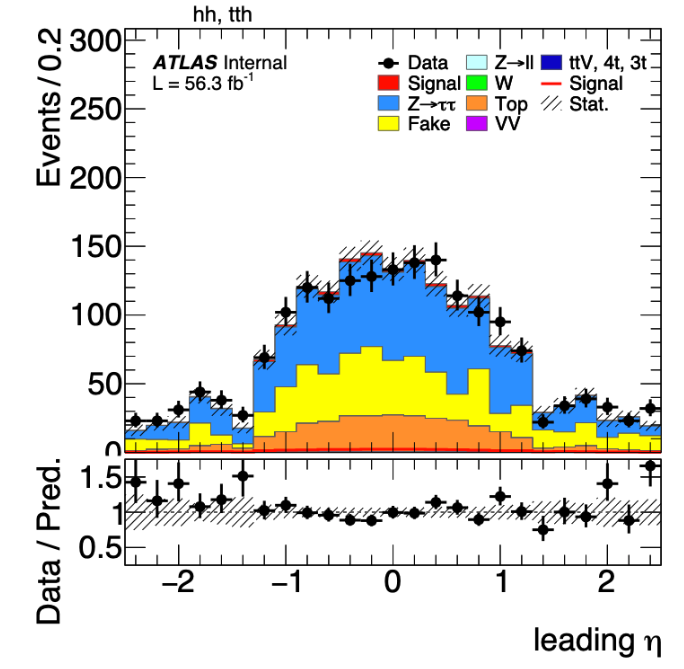
\includegraphics[width=\textwidth]{images/leading_eta_gntau.png}
        \caption{}
    \end{subfigure}

    % Bottom row: RNN
    \begin{subfigure}[b]{0.45\textwidth}
        \centering
        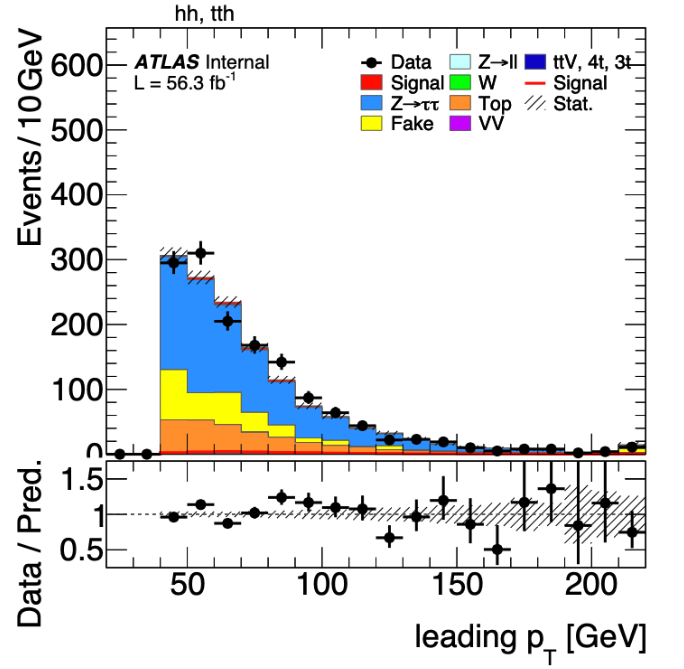
\includegraphics[width=\textwidth]{images/leading_pt_rnn.png}
        \caption{}
    \end{subfigure}
    \begin{subfigure}[b]{0.45\textwidth}
        \centering
        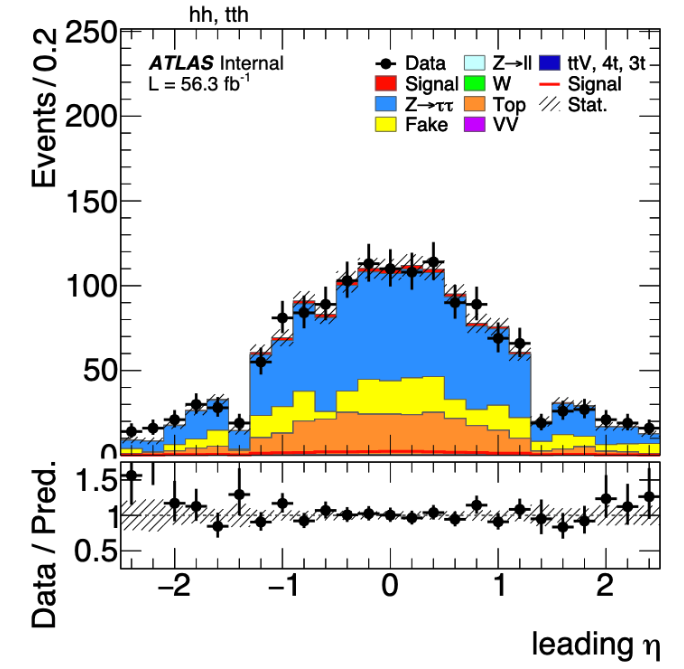
\includegraphics[width=\textwidth]{images/leading_eta_rnn.png}
        \caption{}
    \end{subfigure}

    \caption{Distributions of the leading \tauhad candidate transverse momentum and pseudorapidity at the \ttH preselection with at least one $b$-tagged jet. 
    The upper row shows the results obtained with the new \textsc{GNTau} identification algorithm (a) and (b), while the lower row shows the corresponding distributions with the previously used RNN-based approach (c) and (d). These distributions are evaluated on data and simulations from 2022 data-taking periond.}
    \label{run2_fakes_comparison}
\end{figure}

For this new round, the main variations contributing to the systematic uncertainties in the fake background estimation were recalculated accordingly. In addition to the statistical uncertainties, the composition and parametrization uncertainty sources, already discussed in Section~\ref{sec:event_selection_background}, are also considered.  
To account for differences in background composition as a function of the control region (CR) used to derive the fake factors, two alternative CRs were defined directly in the \tauhadhad final state.  

The first corresponds to the selection of same-sign events, which are naturally enriched in jets misidentified as \tauhad, predominantly originating from QCD multi-jet processes, as mentioned before.
The second alternative is the high-$\Delta\eta(\tau_0,\tau_1)$ region, $1.5 < \Delta\eta < 2.0$, which is more sensitive to dijet-like topologies. In this case, the presence of forward jets with low track multiplicity enhances the probability of jets being misidentified as \tauhad candidates, thus providing an additional validation of the robustness of the method. The closure obtained when estimating this background contribution with these alternative CRs is shown in Figures~\ref{closure_validation_same_sign_run3} and~\ref{closure_validation_same_sign_run2} for the same-sign composition uncertainties, evaluated in the same-sign \tauhadhad signal phase-space, and in Figures~\ref{closure_validation_highdeta_run3} and~\ref{closure_validation_highdeta_run2} it is shown the analogous representation in the high-$\Delta \eta (\tau_0,\tau_1)$ case.
Here it comes some discussion (1-2 lines) mirroring what Serhat said in his thesis.
%Run_3 same_sign closure
\begin{figure}[htbp]
  \centering
  \begin{subfigure}[b]{0.45\textwidth}
    \centering
    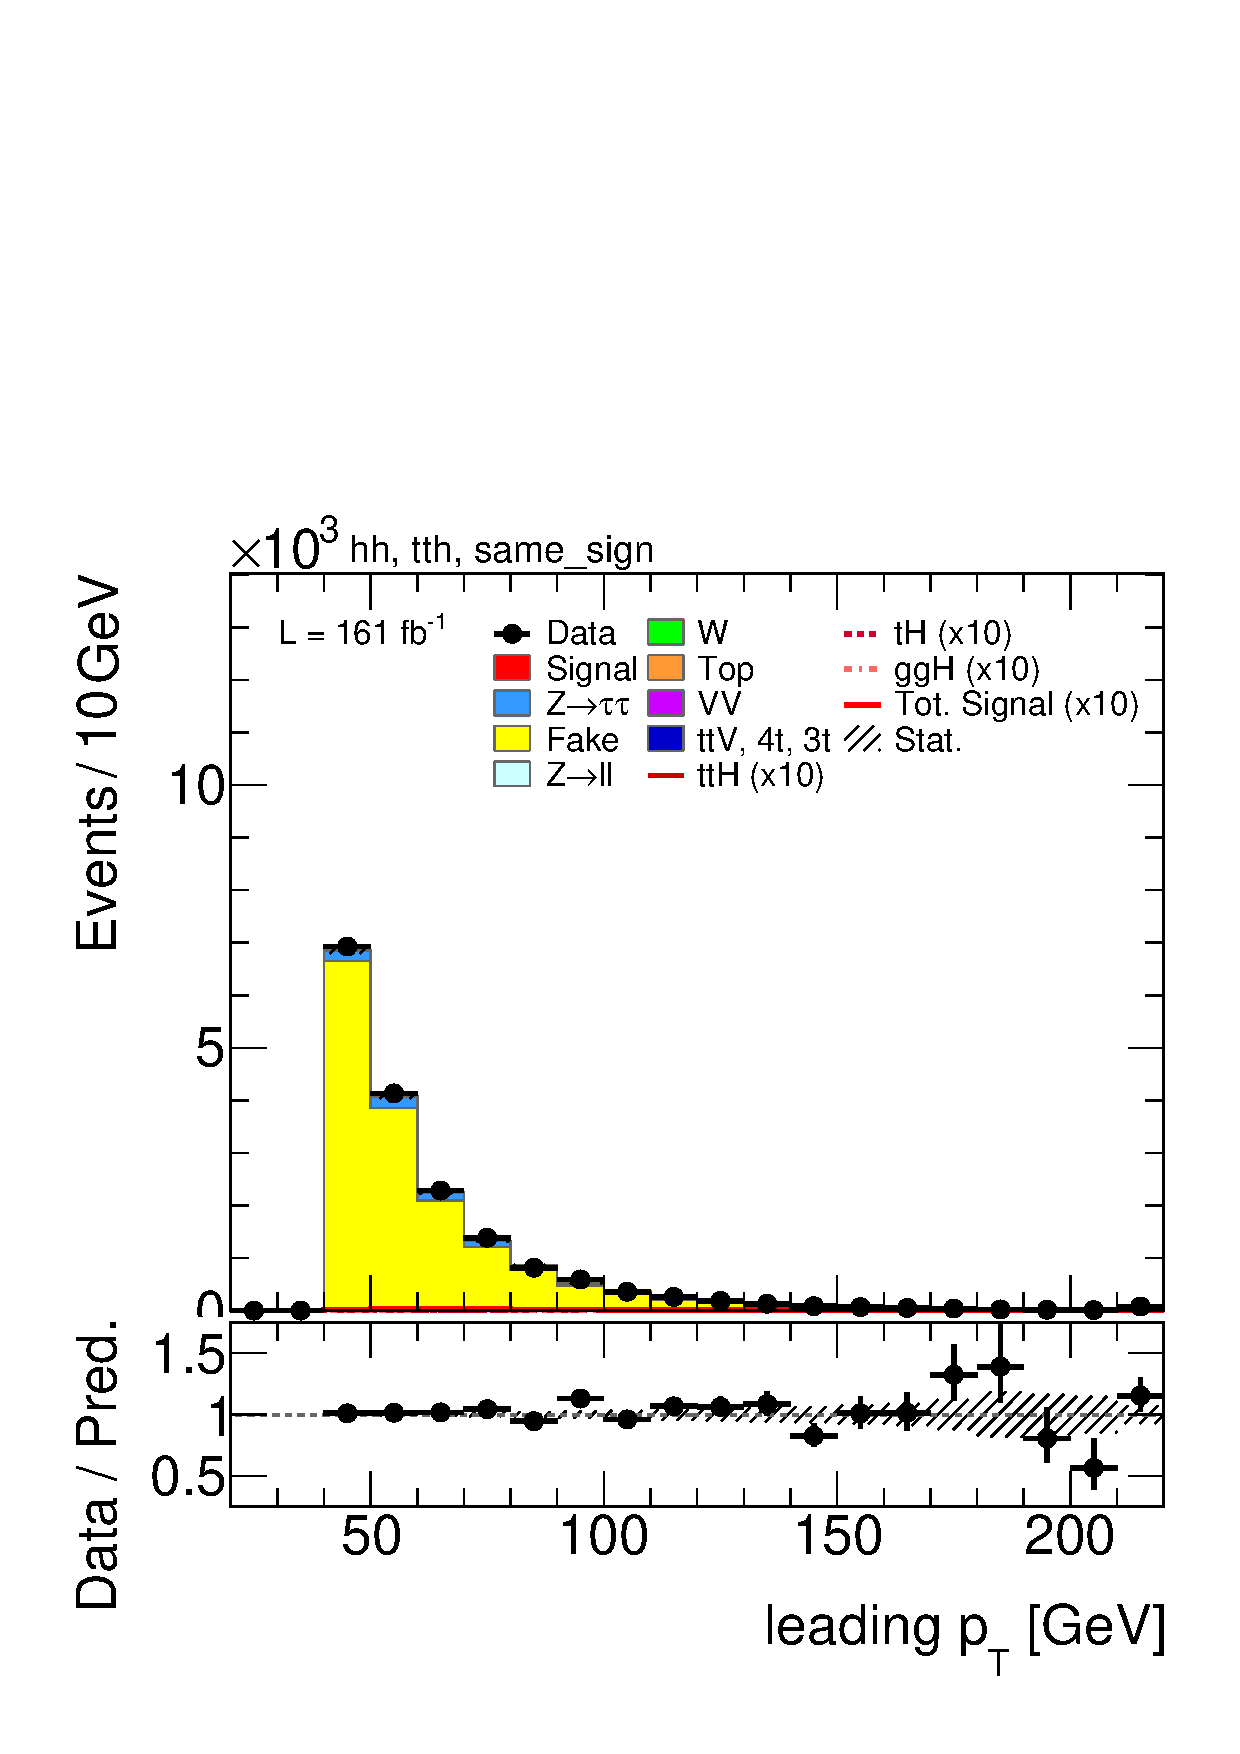
\includegraphics[width=\textwidth]{images/same_sign_same_sign_run3/plot_tau_0_pt_hh_tth_22_23_24_same_sign.pdf}
    \caption{}
  \end{subfigure}
  \hfill
  \begin{subfigure}[b]{0.45\textwidth}
    \centering
    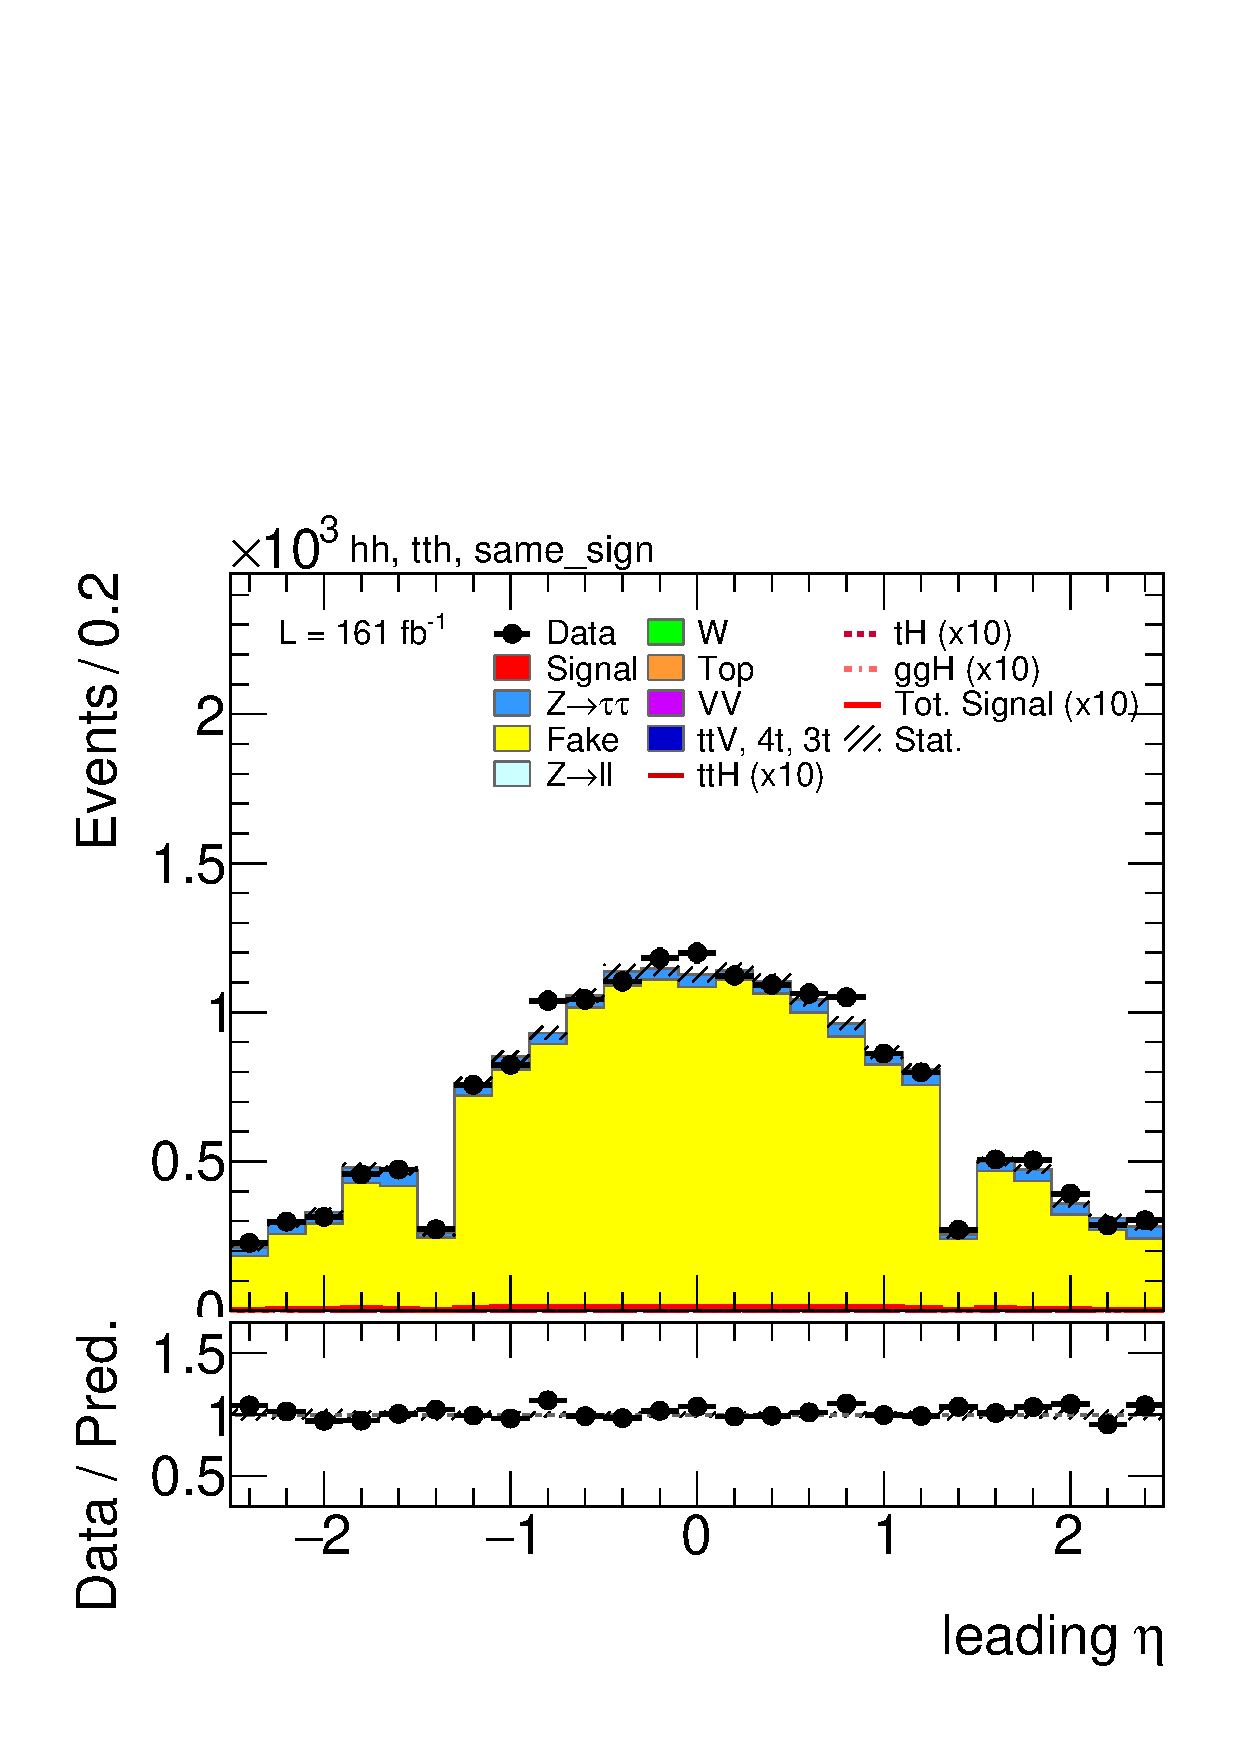
\includegraphics[width=\textwidth]{images/same_sign_same_sign_run3/plot_tau_0_eta_hh_tth_22_23_24_same_sign.pdf}
    \caption{}
  \end{subfigure}


  \begin{subfigure}[b]{0.45\textwidth}
    \centering
    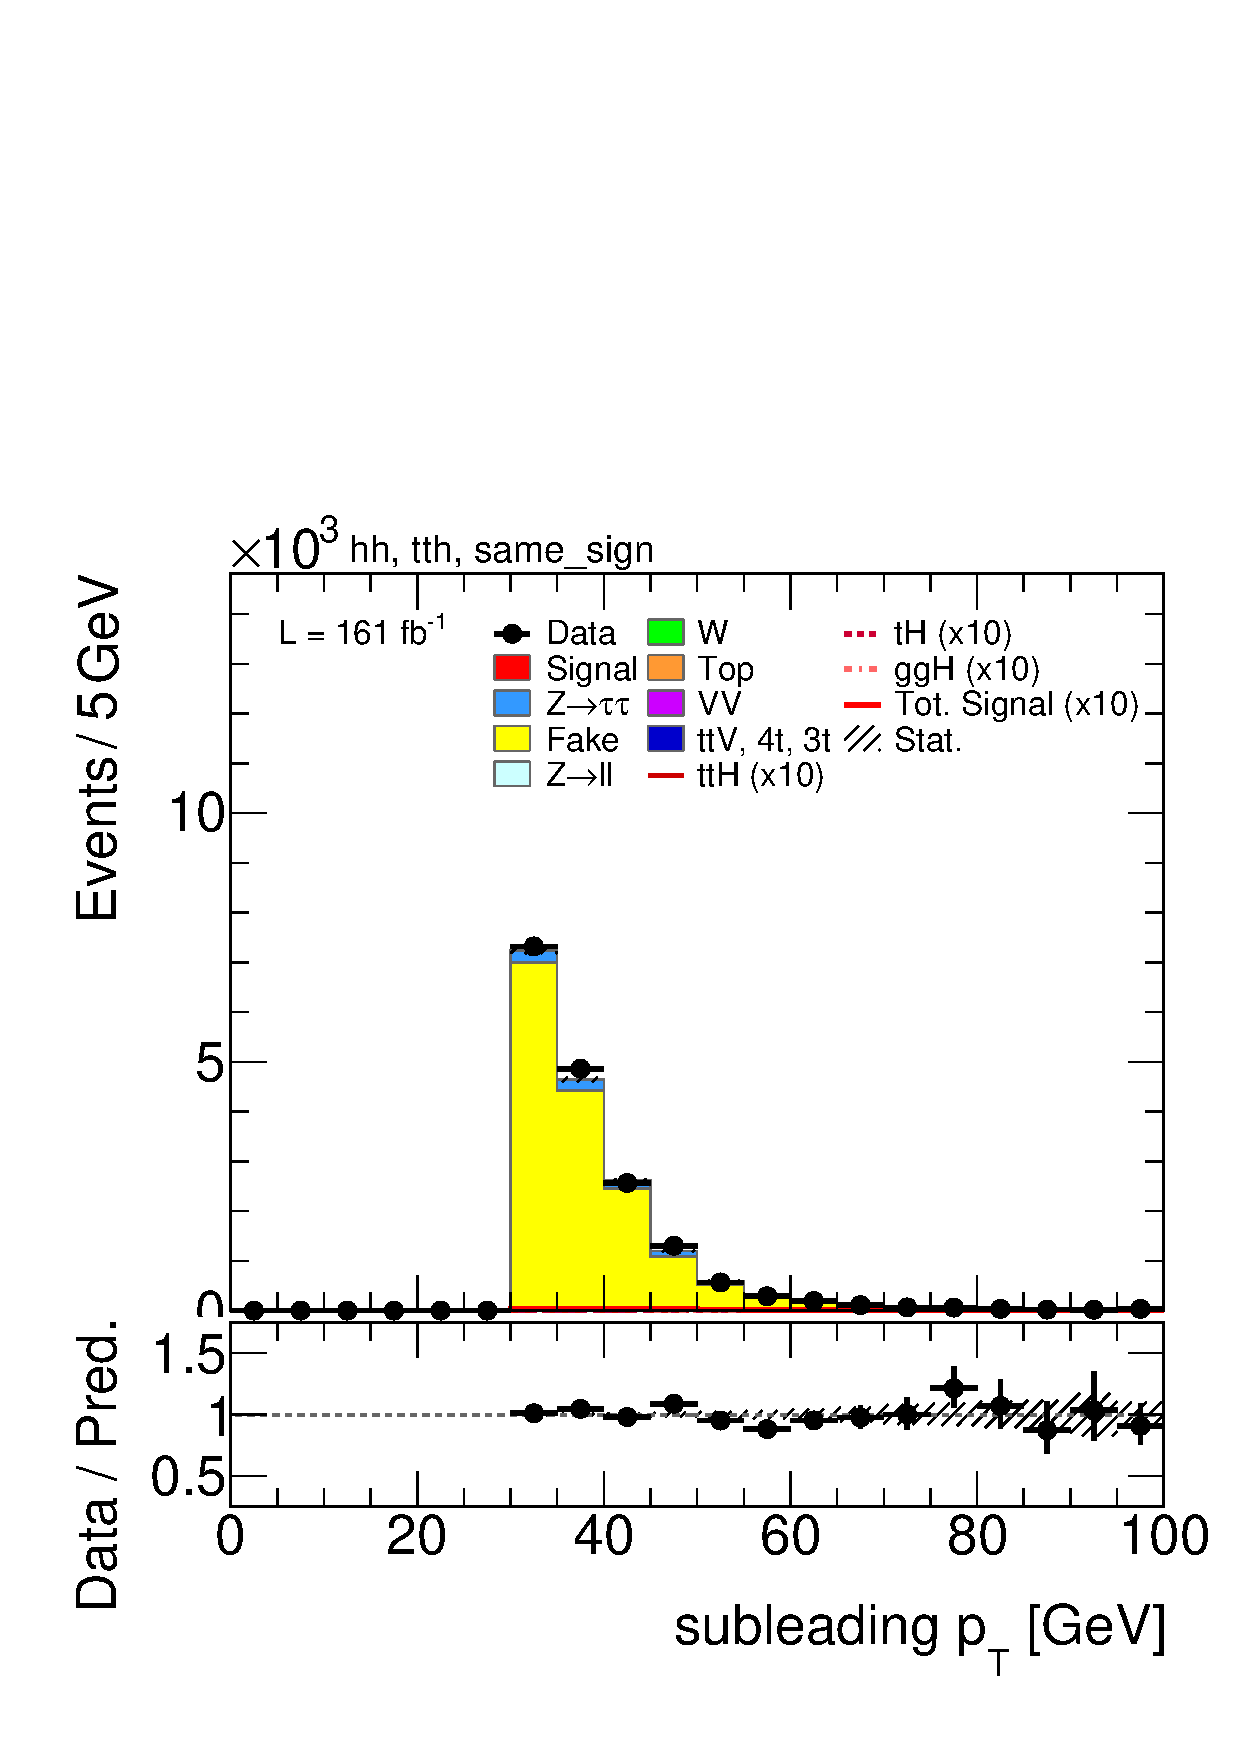
\includegraphics[width=\textwidth]{images/same_sign_same_sign_run3/plot_tau_1_pt_hh_tth_22_23_24_same_sign.pdf}
    \caption{}
  \end{subfigure}
  \hfill
  \begin{subfigure}[b]{0.45\textwidth}
    \centering
    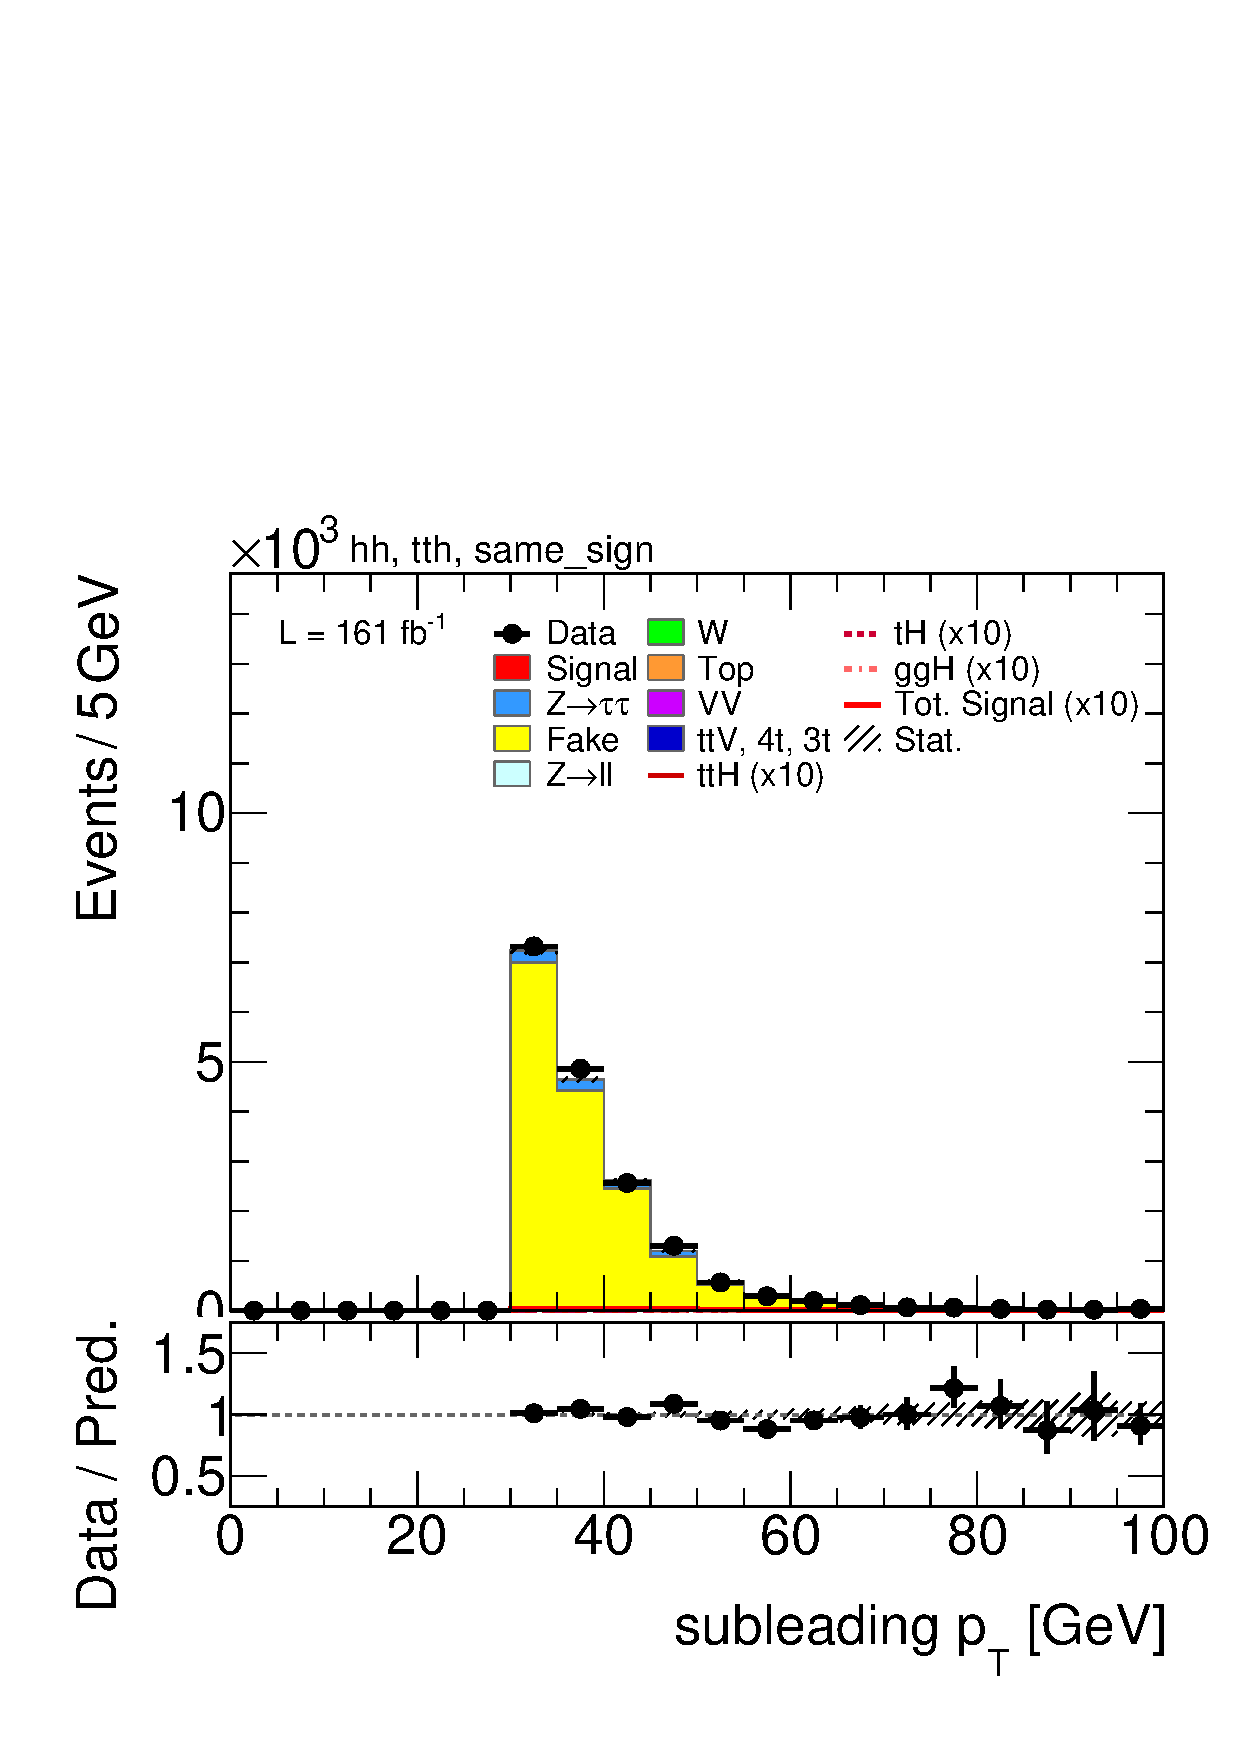
\includegraphics[width=\textwidth]{images/same_sign_same_sign_run3/plot_tau_1_pt_hh_tth_22_23_24_same_sign.pdf}
    \caption{}
  \end{subfigure}
  \caption{
    Closure and validation of the fake background estimated in Run-3 dataset with the alternative same-sign \tauhadhad CR, evaluated in the same-sign region at preselection level.
    The comparison is shown as a function of the \pt and $\eta$ of the leading (a), (b), and subleading (c), (d), \tauhad candidates. 
    Data are compared to the estimated fake background. Scaling factors on \ztautau and \ttbar are applied.
  }
  \label{fig:closure_validation_same_sign_run3}
\end{figure}
  
  
  %Run_2 same_sign closure
  \begin{figure}[htbp]
    \centering
    \begin{subfigure}[b]{0.45\textwidth}
      \centering
      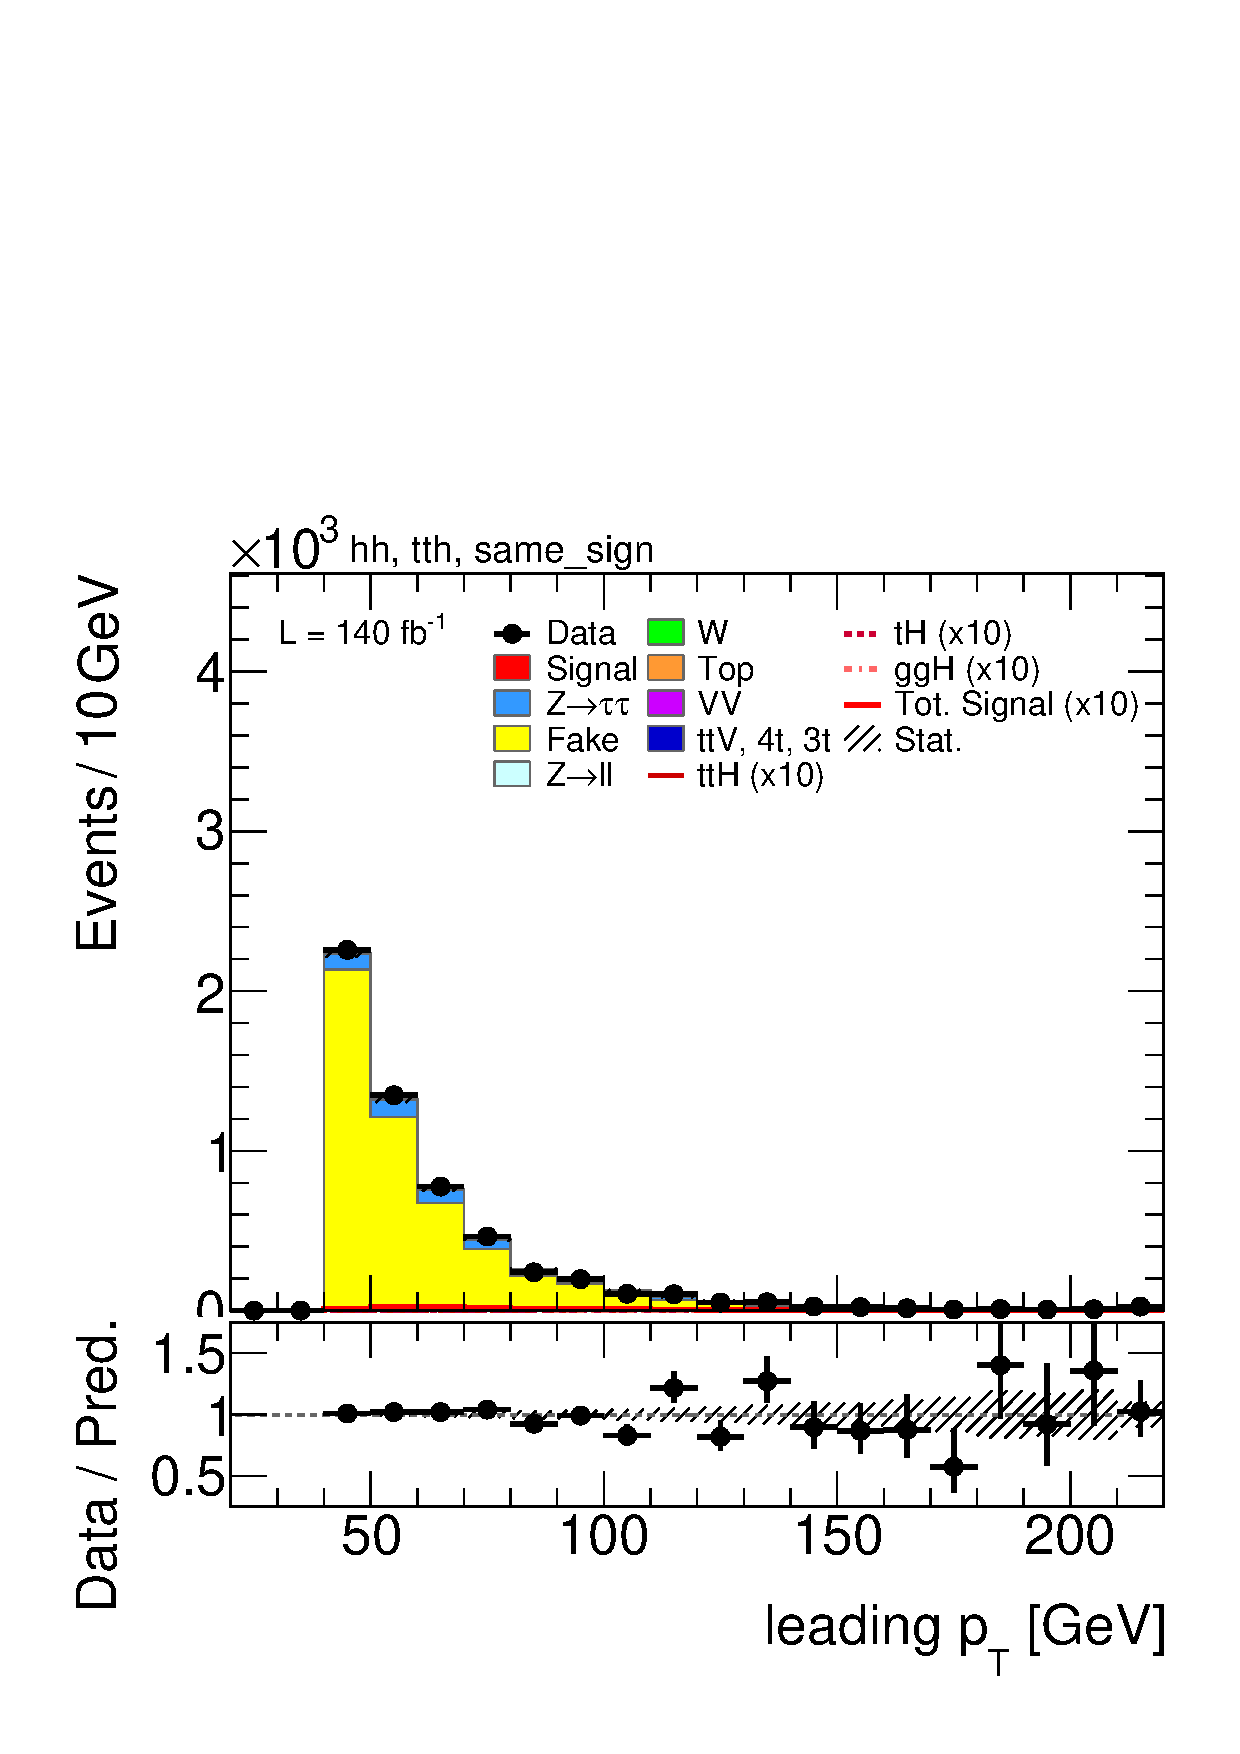
\includegraphics[width=\textwidth]{images/same_sign_same_sign_run2/plot_tau_0_pt_hh_tth_15_16_17_18_same_sign.pdf}
      \caption{}
    \end{subfigure}
    \hfill
    \begin{subfigure}[b]{0.45\textwidth}
      \centering
      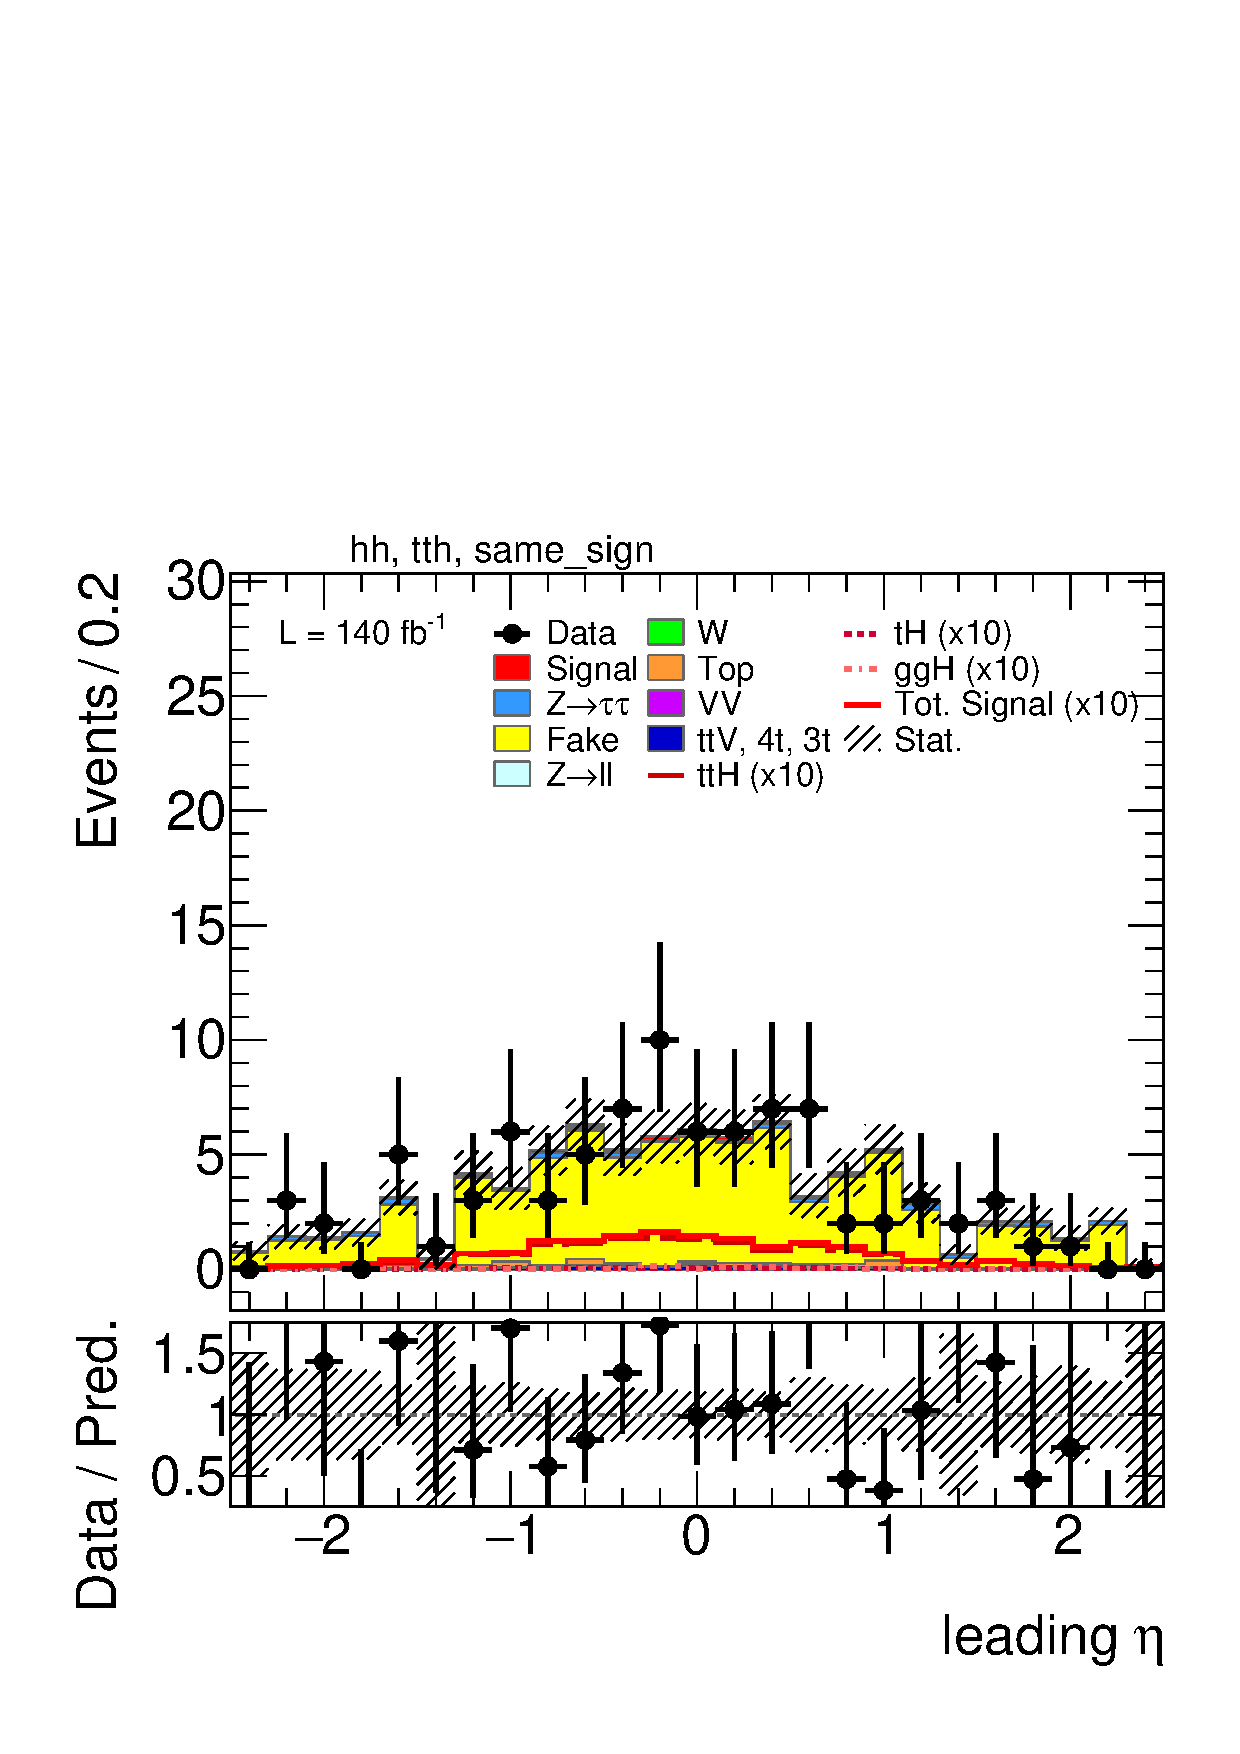
\includegraphics[width=\textwidth]{images/same_sign_same_sign_run2/plot_tau_0_eta_hh_tth_15_16_17_18_same_sign.pdf}
      \caption{}
    \end{subfigure}

    \begin{subfigure}[b]{0.45\textwidth}
      \centering
      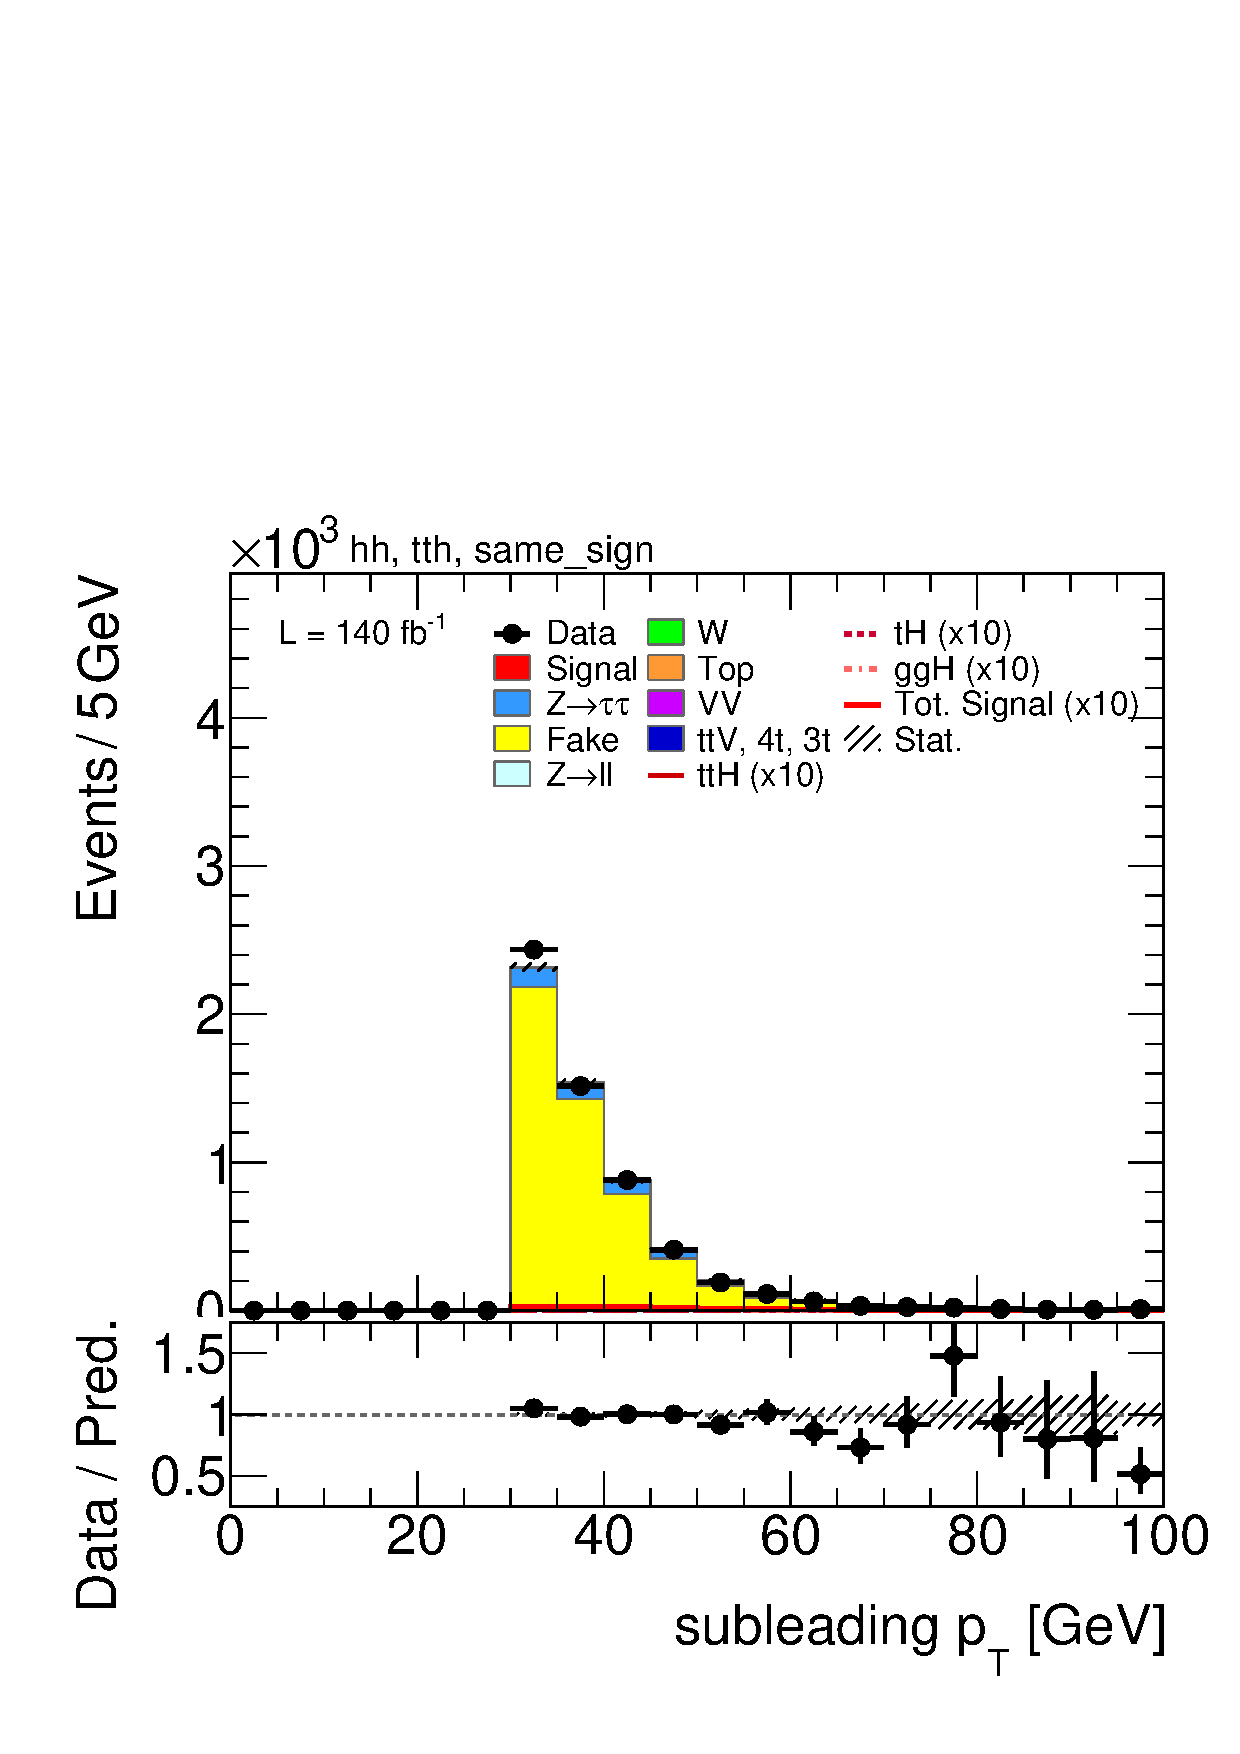
\includegraphics[width=\textwidth]{images/same_sign_same_sign_run2/plot_tau_1_pt_hh_tth_15_16_17_18_same_sign.pdf}
      \caption{}
    \end{subfigure}
    \hfill
    \begin{subfigure}[b]{0.45\textwidth}
      \centering
      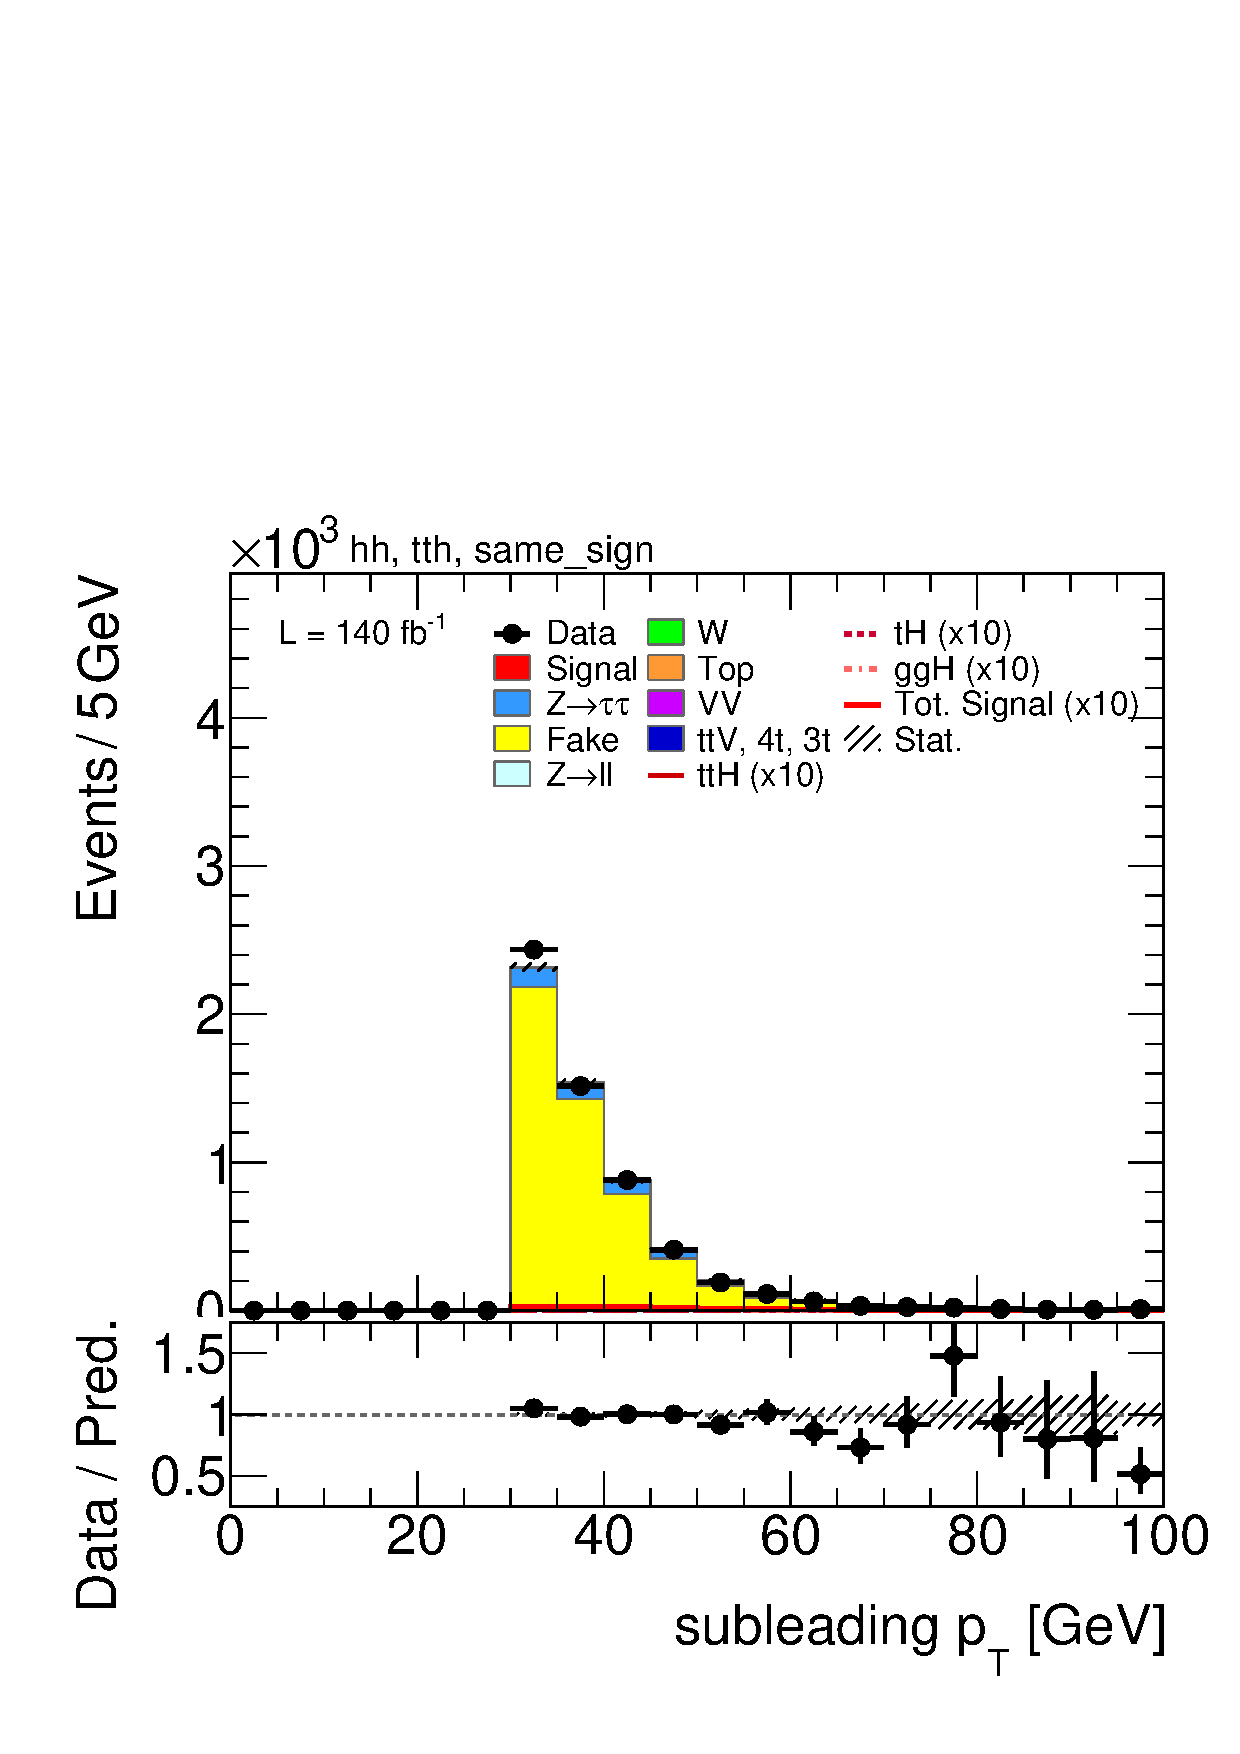
\includegraphics[width=\textwidth]{images/same_sign_same_sign_run2/plot_tau_1_pt_hh_tth_15_16_17_18_same_sign.pdf}
      \caption{}
    \end{subfigure}

    \caption{
    Closure and validation of the fake background estimated in Run-2 dataset with the alternative same-sign \tauhadhad CR, evaluated in the same-sign region at preselection level.
    The comparison is shown as a function of the \pt and $\eta$ of the leading (a), (b), and subleading (c), (d), \tauhad candidates. 
    Data are compared to the estimated fake background.
  }
  \label{fig:closure_validation_same_sign_run2}
\end{figure}

    %Run_3 high_deta closure
    \begin{figure}[htbp]
      \centering
      \begin{subfigure}[b]{0.45\textwidth}
        \centering
        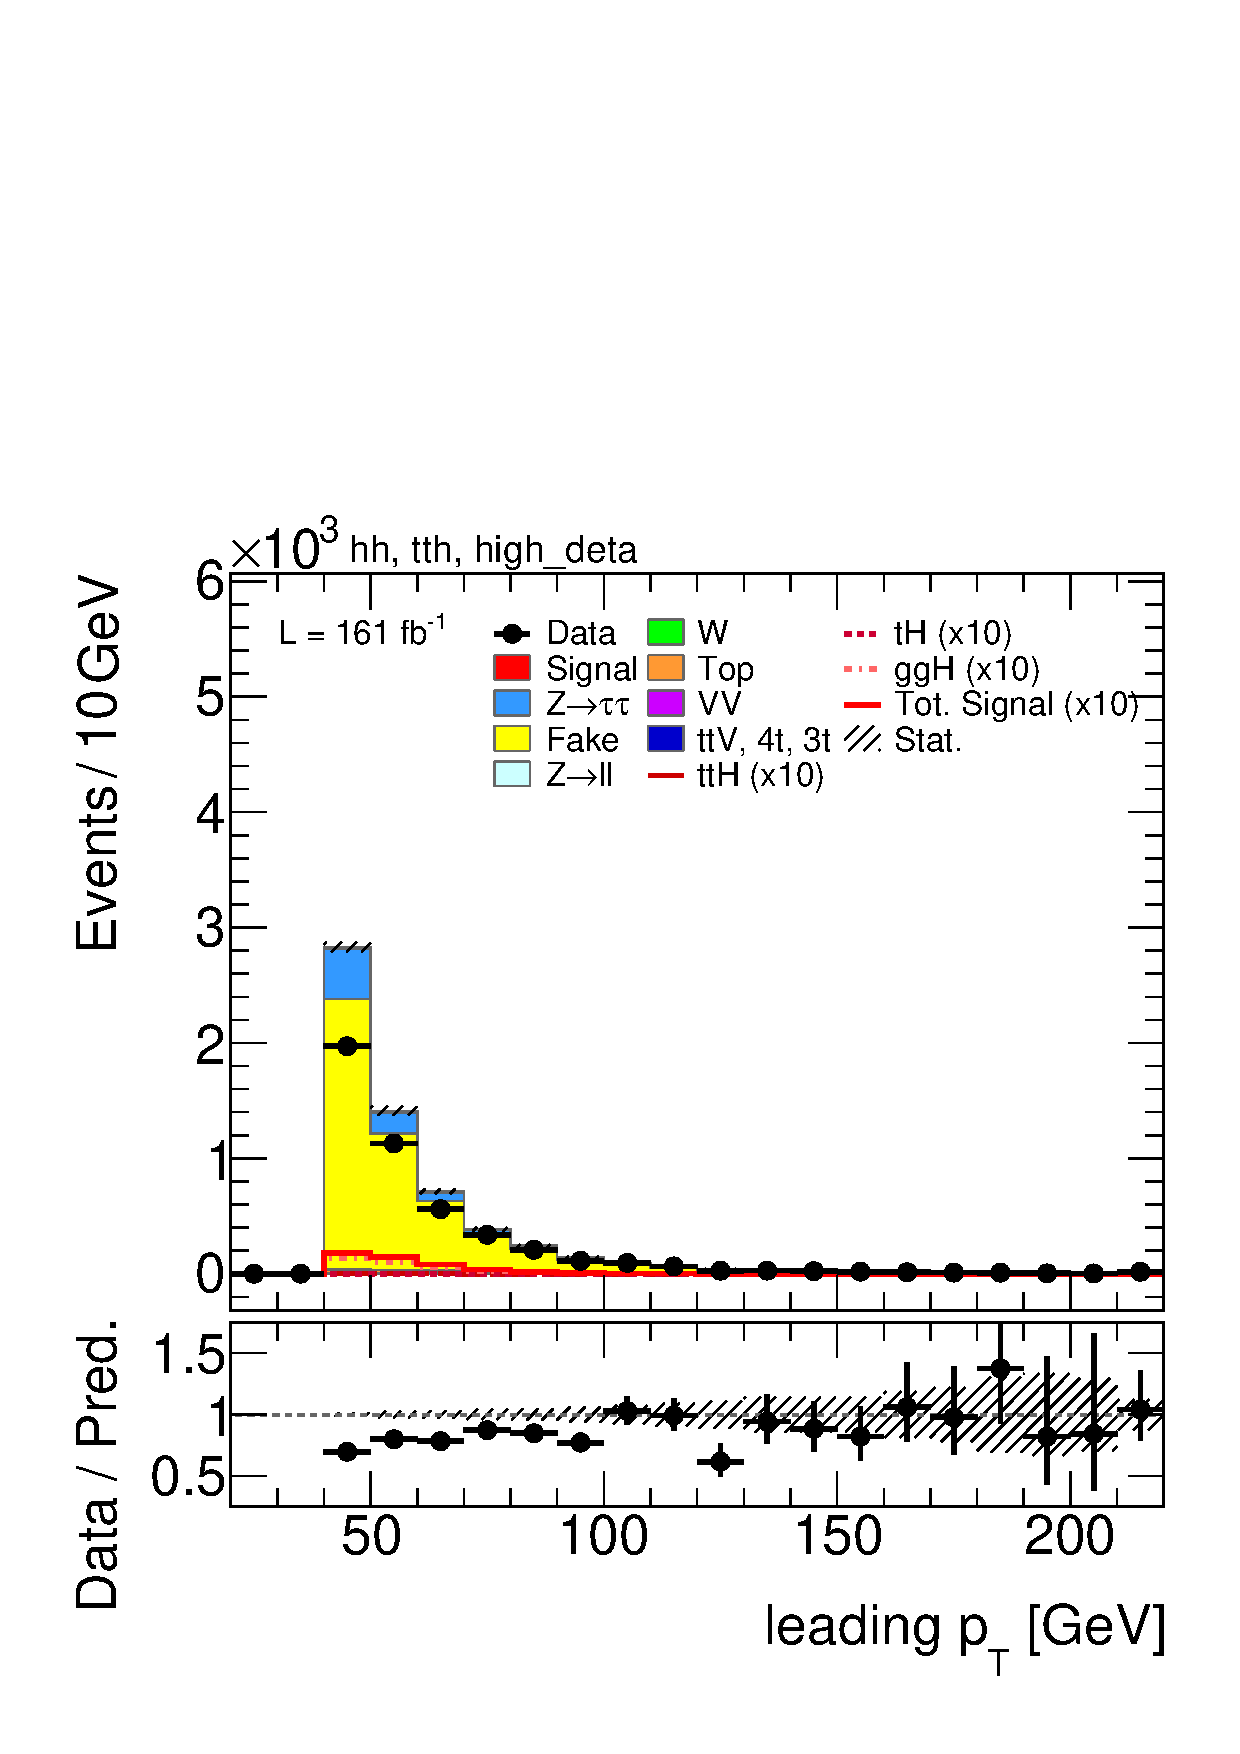
\includegraphics[width=\textwidth]{images/highdeta_highdeta_run3/plot_tau_0_pt_hh_tth_22_23_24_high_deta.pdf}
        \caption{}
      \end{subfigure}
      \hfill
      \begin{subfigure}[b]{0.45\textwidth}
        \centering
        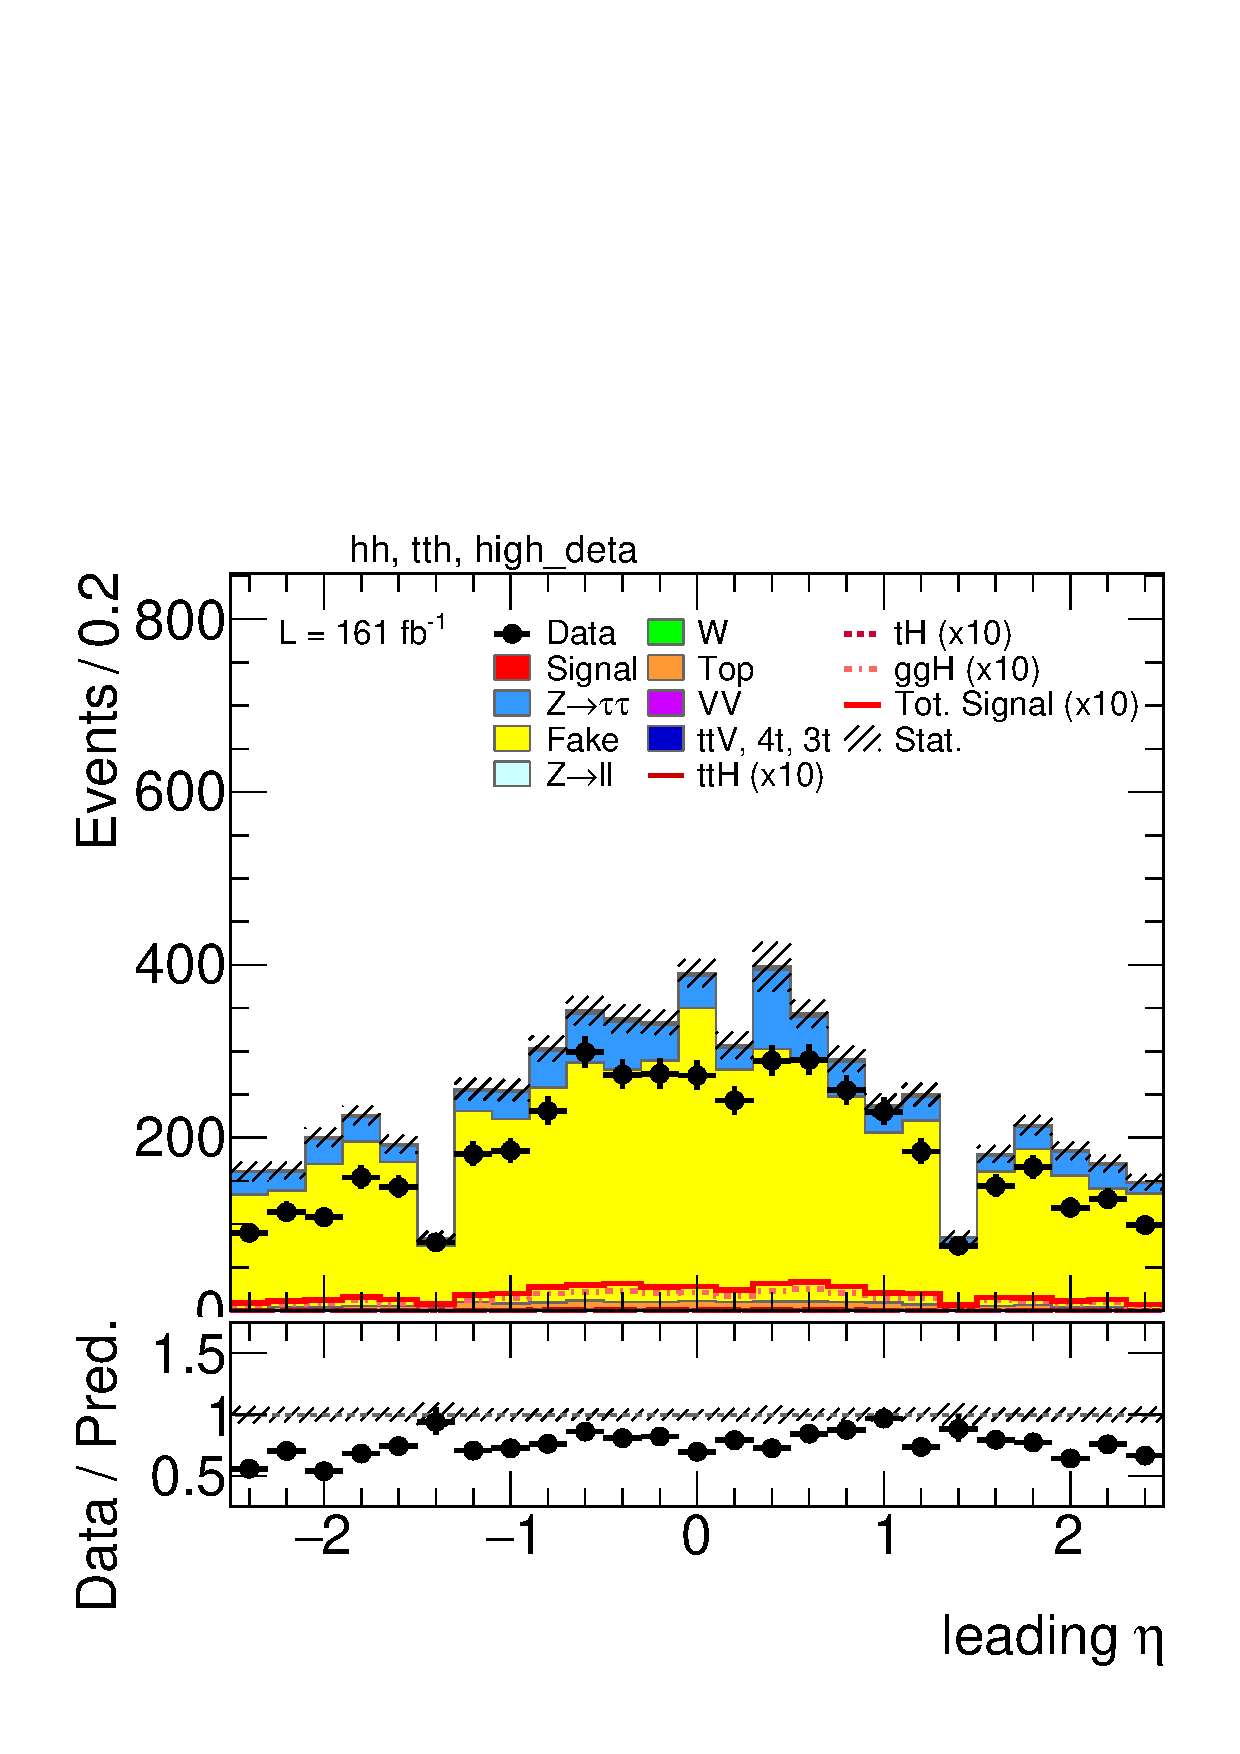
\includegraphics[width=\textwidth]{images/highdeta_highdeta_run3/plot_tau_0_eta_hh_tth_22_23_24_high_deta.pdf}
        \caption{}
      \end{subfigure}
  
      \begin{subfigure}[b]{0.45\textwidth}
        \centering
        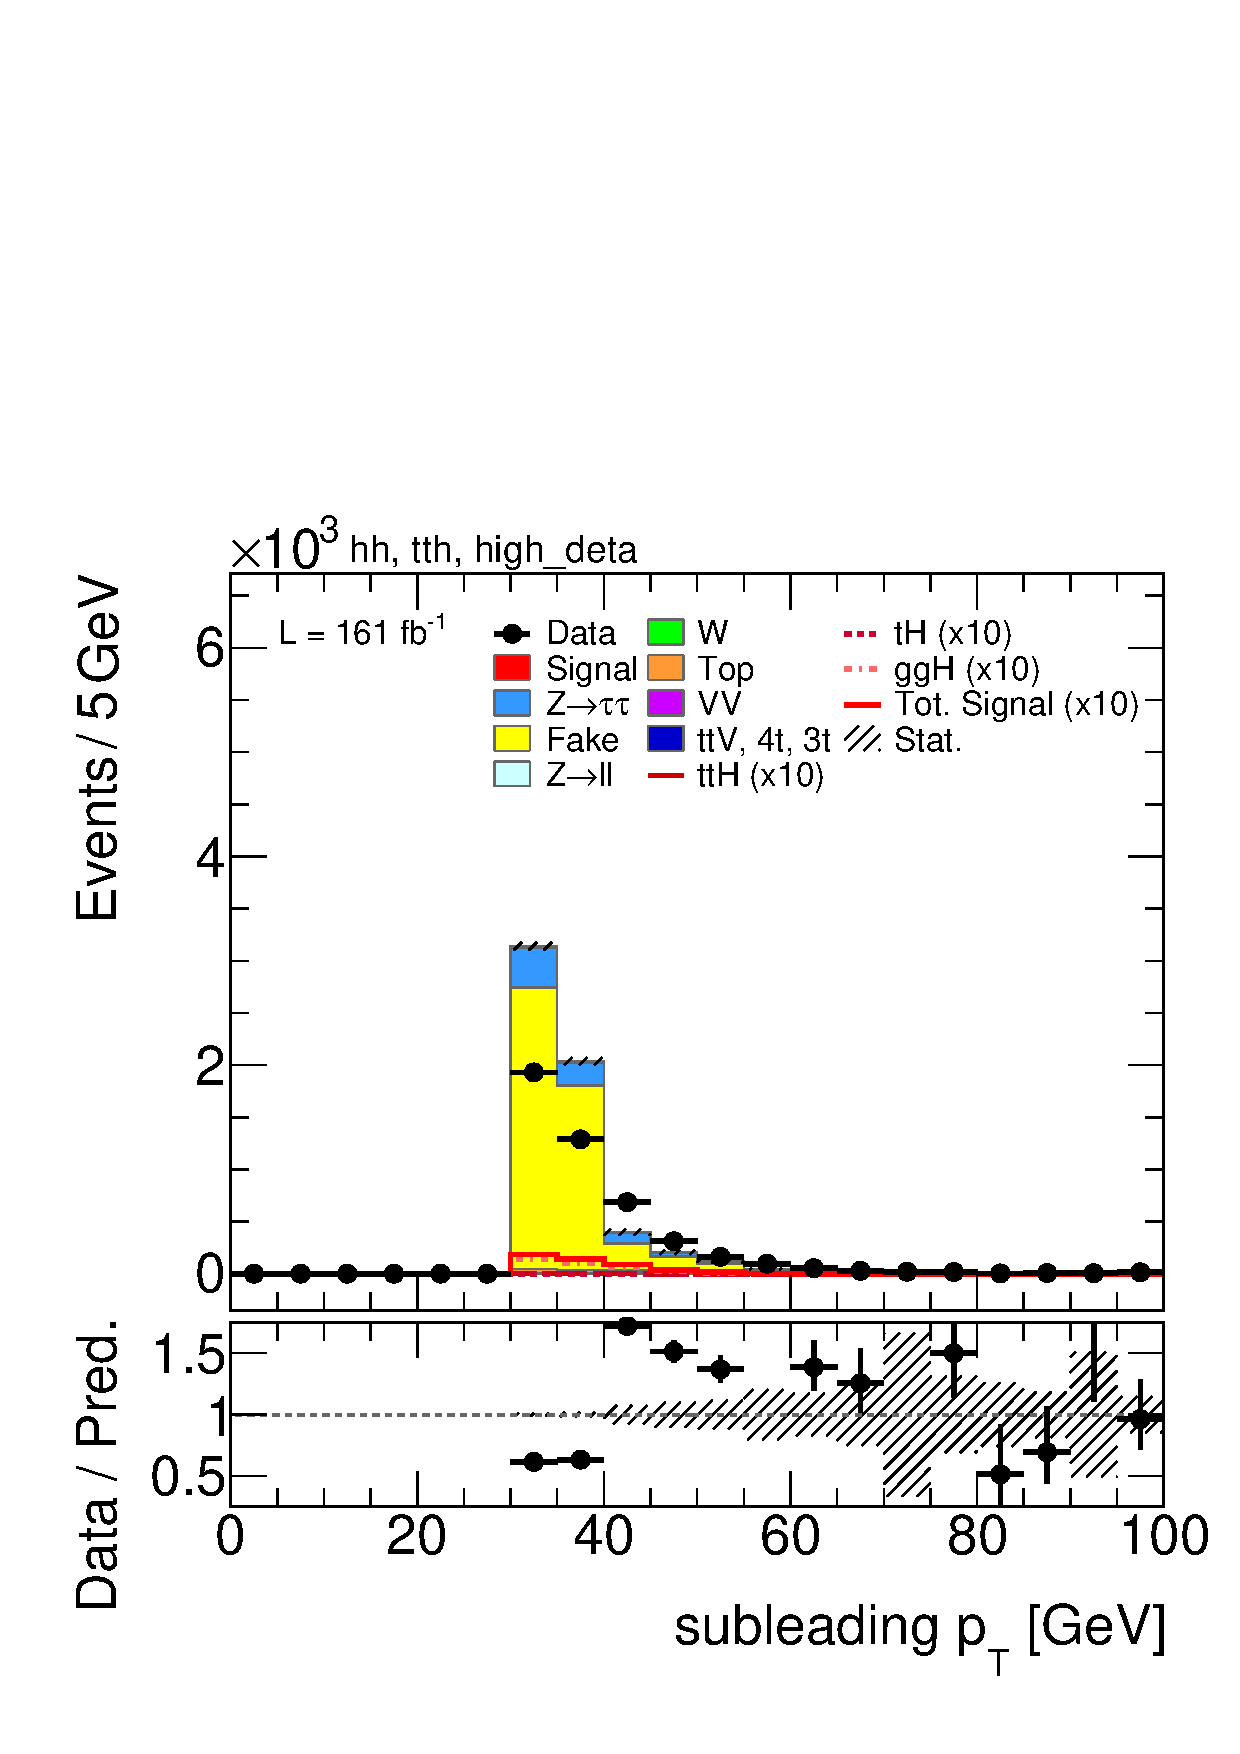
\includegraphics[width=\textwidth]{images/highdeta_highdeta_run3/plot_tau_1_pt_hh_tth_22_23_24_high_deta.pdf}
        \caption{}
      \end{subfigure}
      \hfill
      \begin{subfigure}[b]{0.45\textwidth}
        \centering
        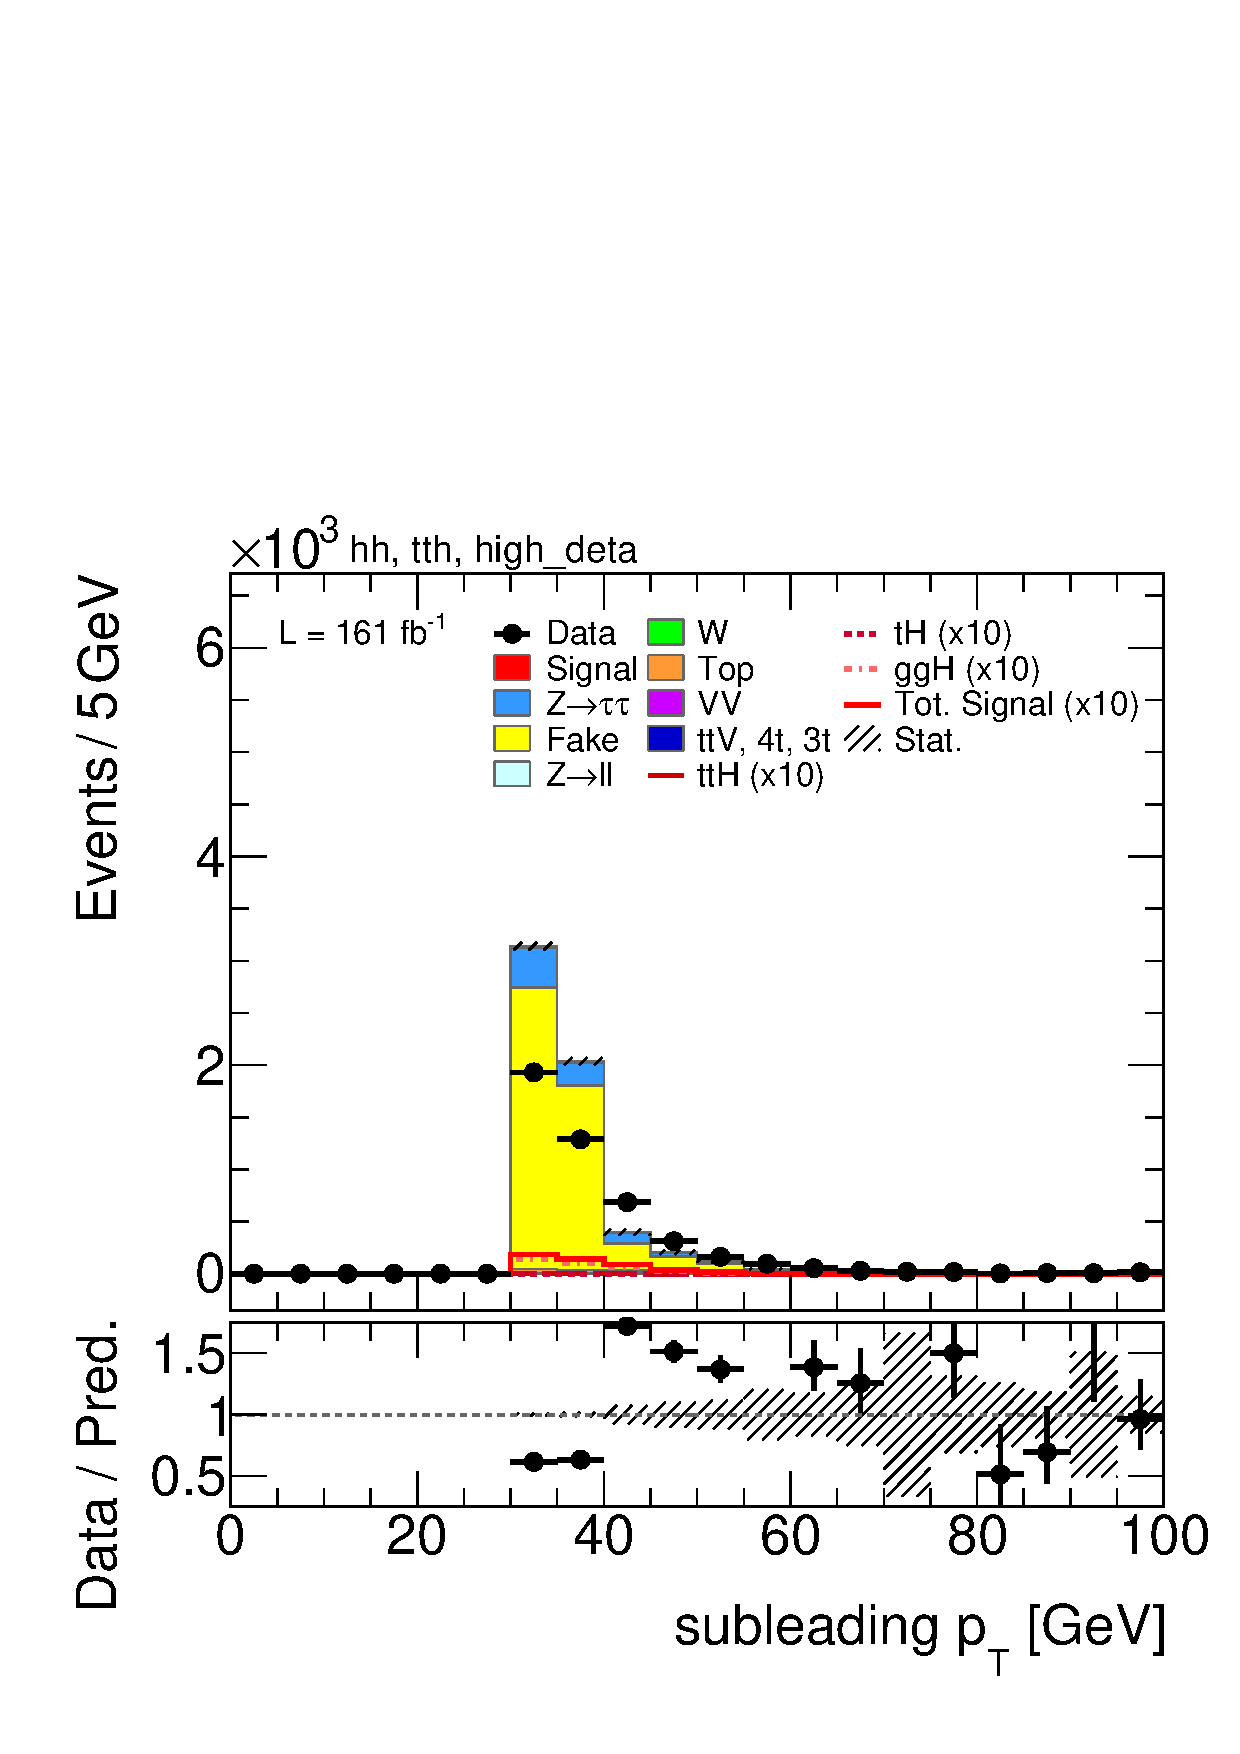
\includegraphics[width=\textwidth]{images/highdeta_highdeta_run3/plot_tau_1_pt_hh_tth_22_23_24_high_deta.pdf}
        \caption{}
      \end{subfigure}
      \caption{
    Closure and validation of the fake background estimated in Run-3 dataset with the alternative high-$\Delta \eta (\tau_0, \tau_1)$ \tauhadhad CR, evaluated in the high-$\Delta \eta (\tau_0, \tau_1)$ region at preselection level.
    The comparison is shown as a function of the \pt and $\eta$ of the leading (a), (b), and subleading (c), (d), \tauhad candidates. 
    Data are compared to the estimated fake background. Scaling factors on \ztautau and \ttbar are applied.
  }
  \label{fig:closure_validation_highdeta_run3}
\end{figure}
      

      %Run_2 high_deta closure
      \begin{figure}[htbp]
        \centering
        \begin{subfigure}[b]{0.45\textwidth}
          \centering
          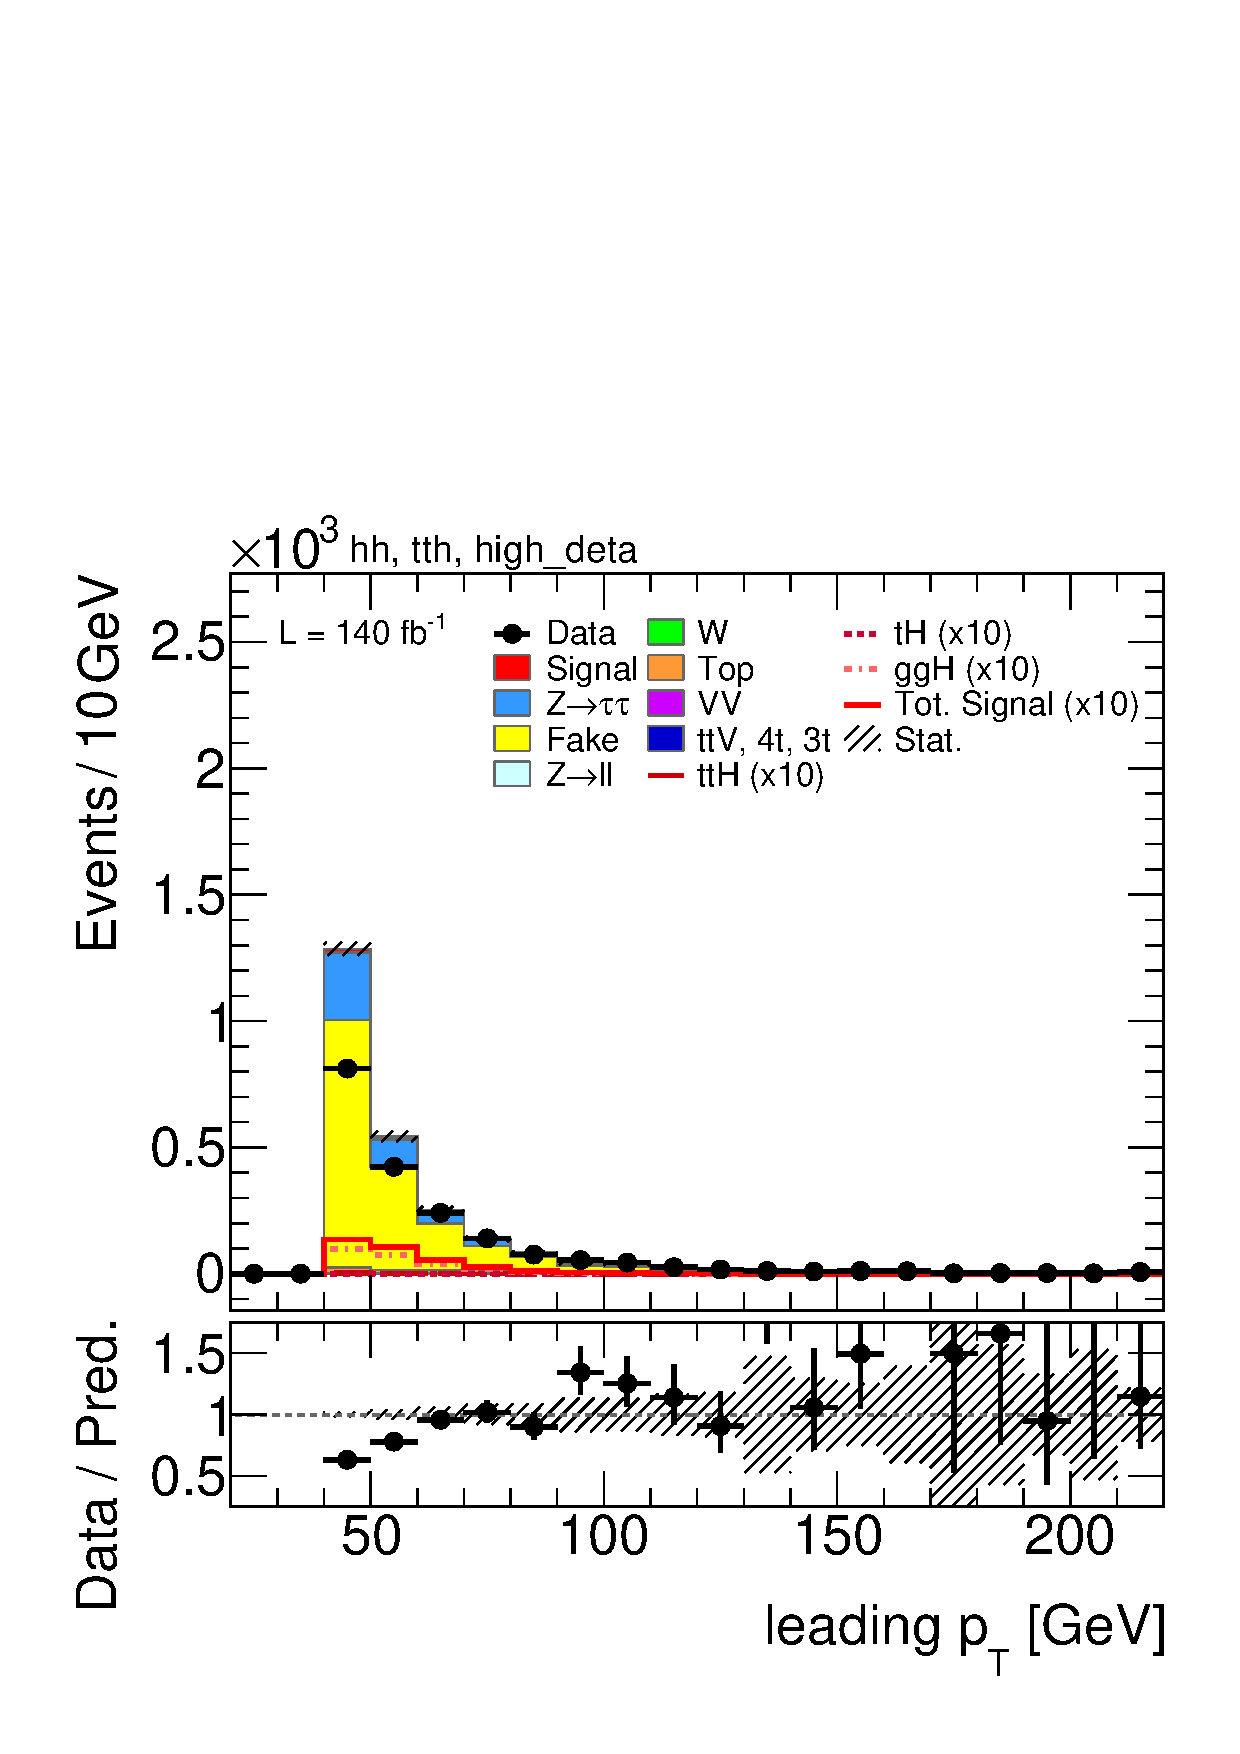
\includegraphics[width=\textwidth]{images/highdeta_highdeta_run2/plot_tau_0_pt_hh_tth_15_16_17_18_high_deta.pdf}
          \caption{}
        \end{subfigure}
        \hfill
        \begin{subfigure}[b]{0.45\textwidth}
          \centering
          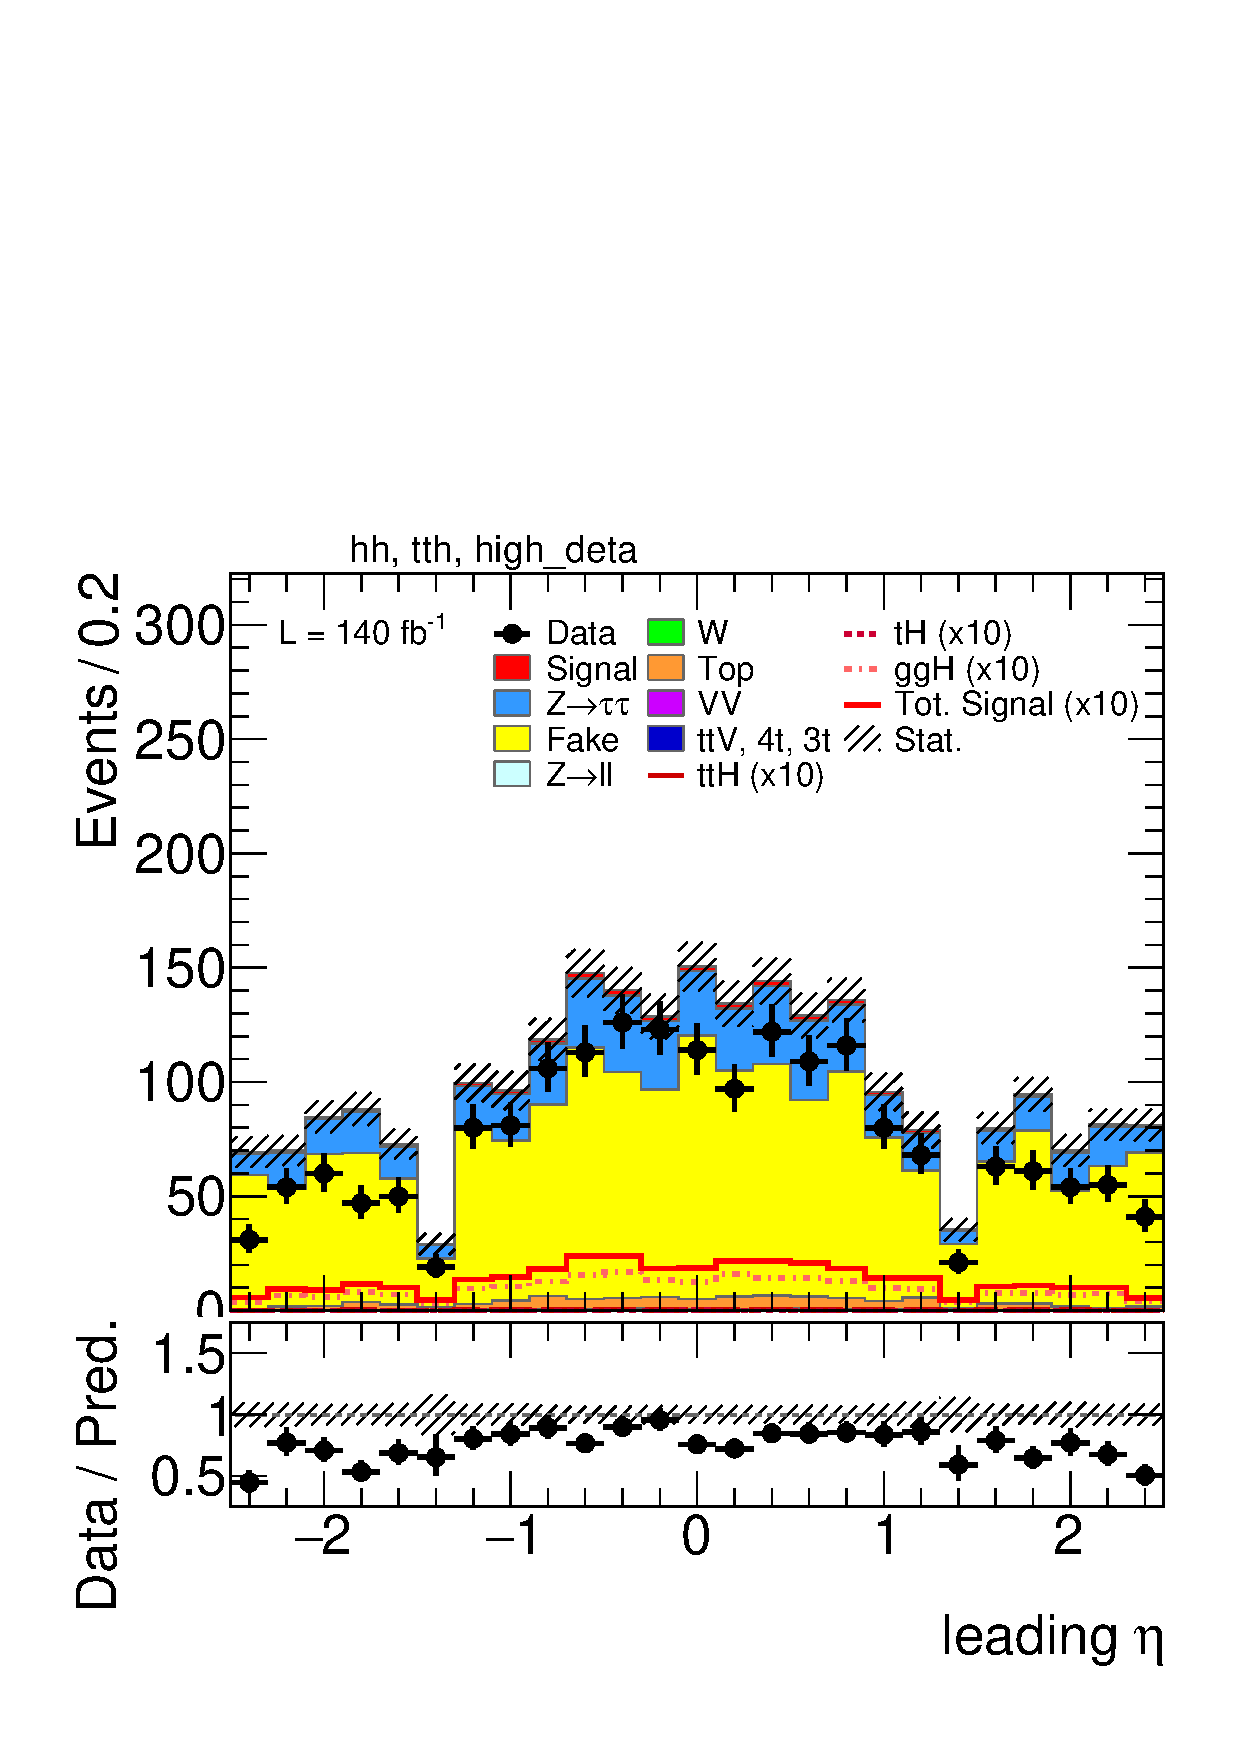
\includegraphics[width=\textwidth]{images/highdeta_highdeta_run2/plot_tau_0_eta_hh_tth_15_16_17_18_high_deta.pdf}
          \caption{}
        \end{subfigure}
    
        \begin{subfigure}[b]{0.45\textwidth}
          \centering
          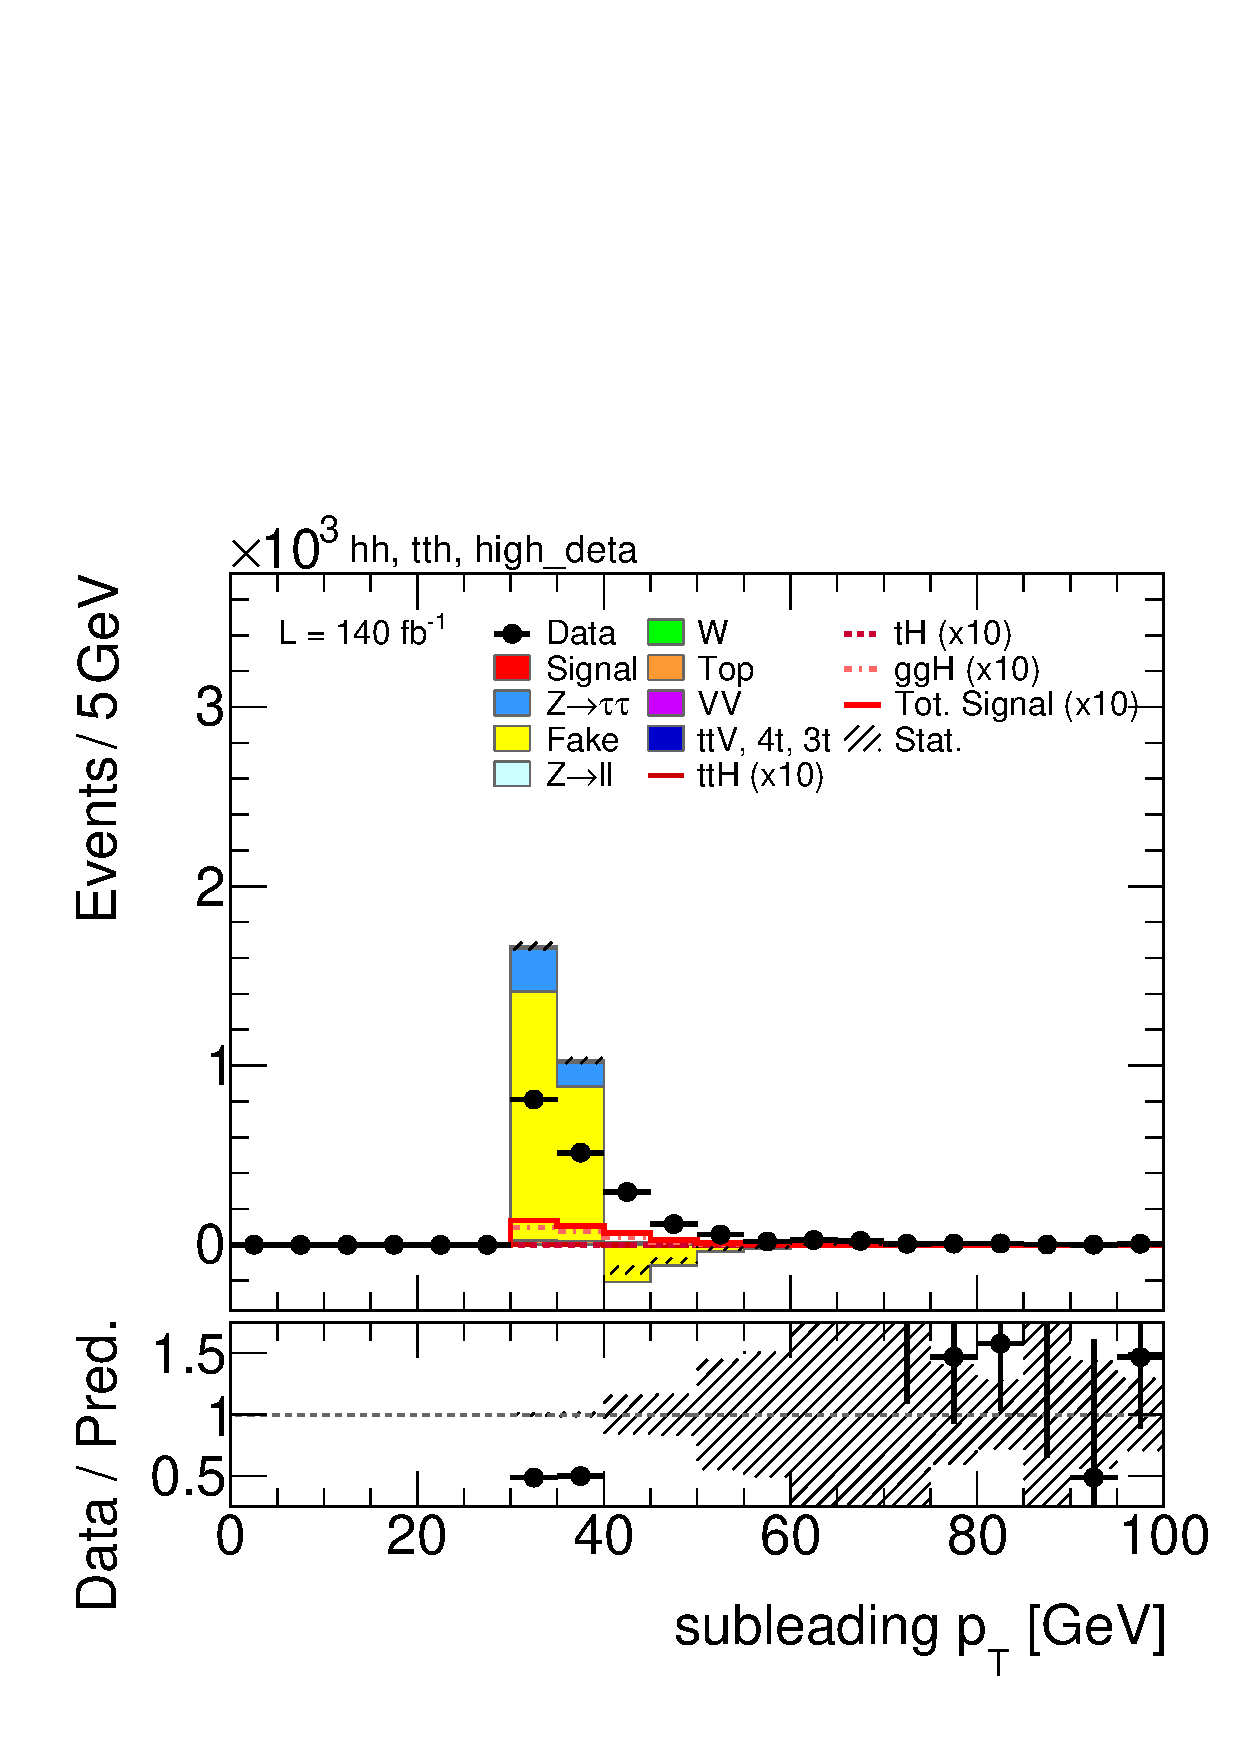
\includegraphics[width=\textwidth]{images/highdeta_highdeta_run2/plot_tau_1_pt_hh_tth_15_16_17_18_high_deta.pdf}
          \caption{}
        \end{subfigure}
        \hfill
        \begin{subfigure}[b]{0.45\textwidth}
          \centering
          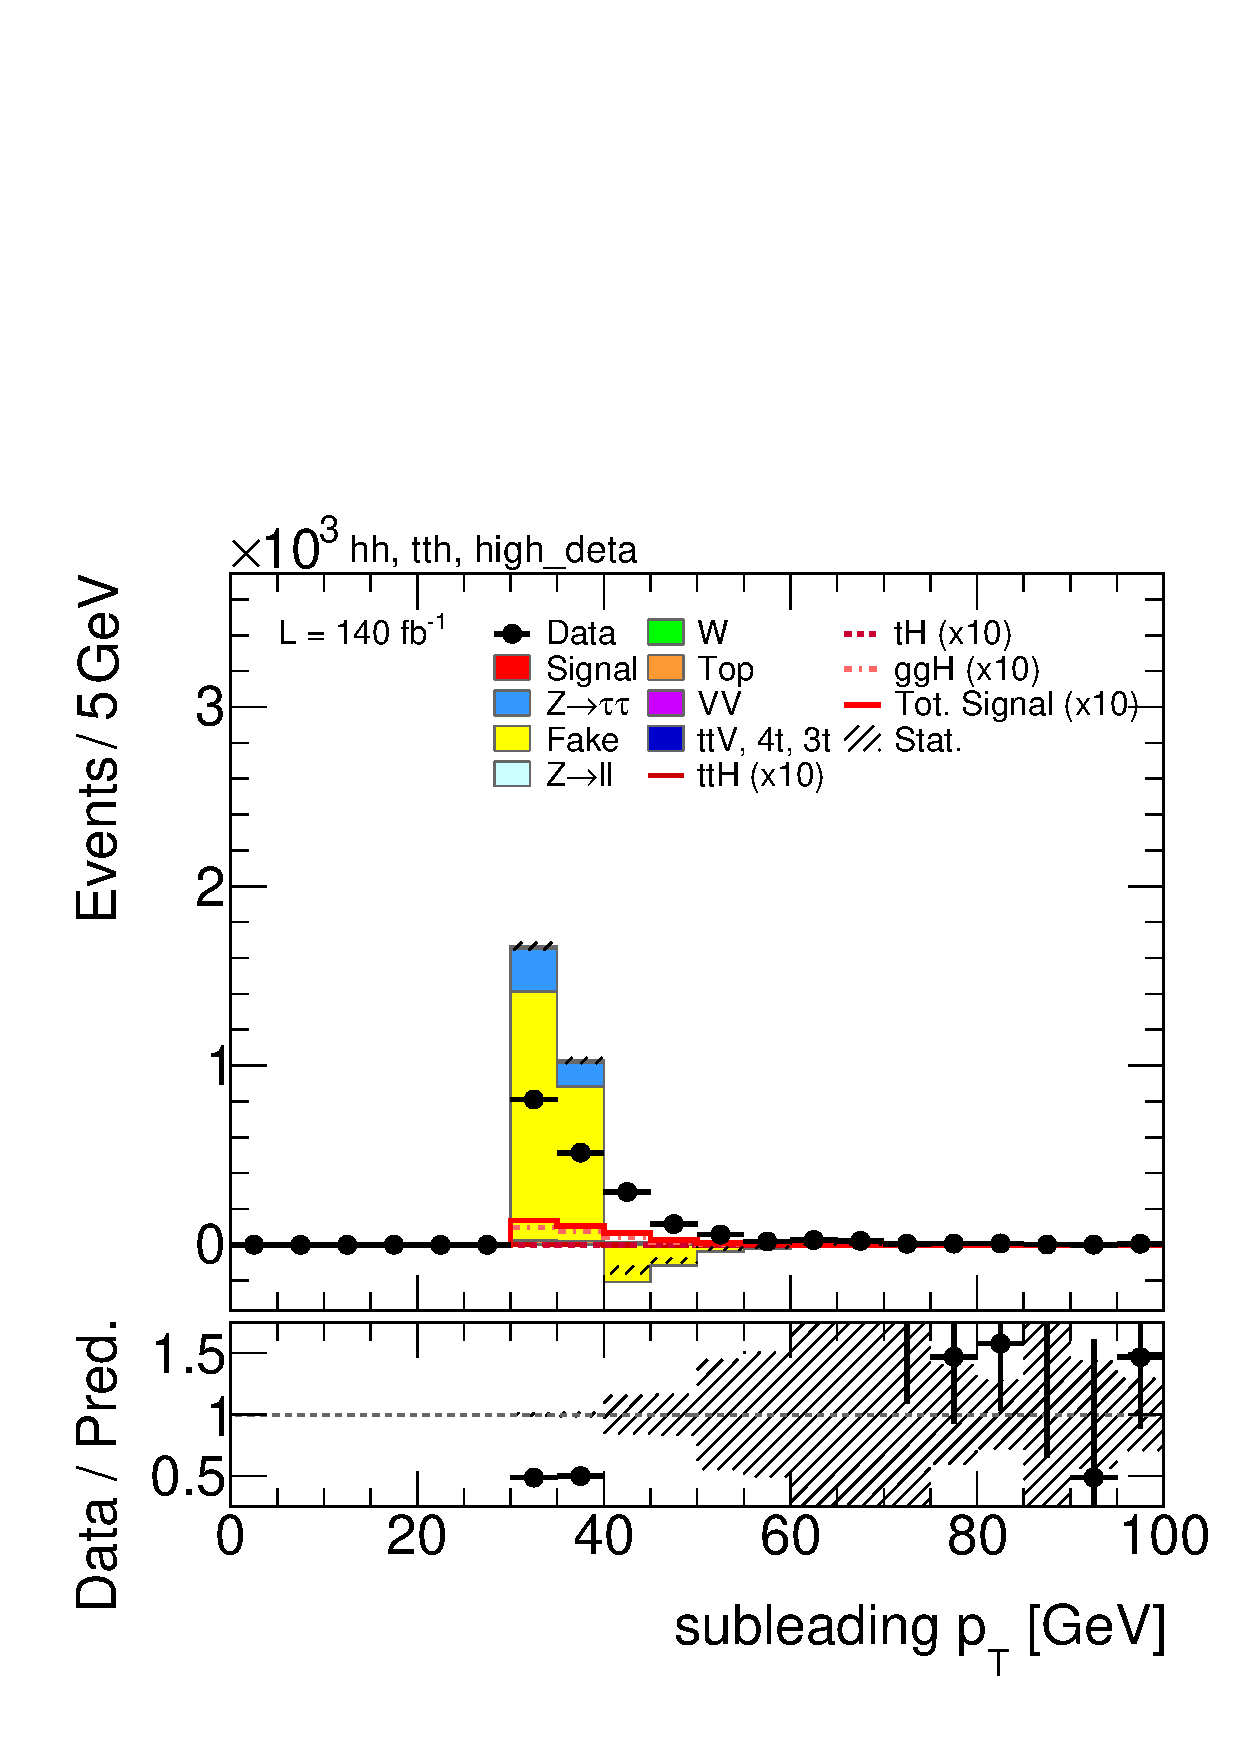
\includegraphics[width=\textwidth]{images/highdeta_highdeta_run2/plot_tau_1_pt_hh_tth_15_16_17_18_high_deta.pdf}
          \caption{}
        \end{subfigure}
        \caption{
    Closure and validation of the fake background estimated in Run-2 dataset with the alternative high-$\Delta \eta (\tau_0, \tau_1)$ \tauhadhad CR, evaluated in the high-$\Delta \eta (\tau_0, \tau_1)$ region at preselection level.
    The comparison is shown as a function of the \pt and $\eta$ of the leading (a), (b), and subleading (c), (d), \tauhad candidates. 
    Data are compared to the estimated fake background.
  }
  \label{fig:closure_validation_highdeta_run2}
\end{figure}

The remaining source of uncertainty in the estimation of this background can be referred to as the parametrization uncertainty. This is re-derived, although it has only a minor impact on the analysis, by evaluating the effect of estimating the background contribution using fake factors calculated separately for the leading and subleading \tauhad candidates in the \tauhadhad same-sign region, which then need to be combined, instead of relying on a single nominal fake factor calculated in the \taulephad W+jets CR. The procedure followed to estimate these variations is described in Ref.~\cite{serhat_tesis}.
  



\section{New MVA strategy for event categorization}

The strategy adopted in this new analysis for the further classification of events of interest within the defined phase space closely follows the approach discussed in Section~\ref{sec:tth_mva}. The same multiclass BDT algorithm is employed, but in this case it is extended to a total of four classes, including an additional one for the \thtt signal.
It should be emphasised that an inclusive training in \pth is carried out at this stage. The objective is not to perform a statistical fit targeting different STXS phase space bins in order to refine the precision of the measurements, but rather to obtain a combined study of \ttH and \thqb, with the aim of assessing the potential sensitivity achievable for this newly incorporated production mode.

\subsection{New 4-class BDT}
Originally, the strategy would rely on employing as input variables the same list that had previously been used to separate \ttH from \ztautau and from \ttbar, since the features exploited to distinguish these final states are also expected to provide separation power for a second signal process, \thqb.
Nevertheless, as already discussed, the topologies of \ttHtt and \thtt are very similar, and their separation must be maximised. This is particularly relevant given that in both cases two \tauhad originate from the Higgs boson decay, the final state contains multiple jets, and $b$-jets emerge from the top-quark decay.

To enhance the separation of the two signal processes, a set of additional variables is therefore incorporated. These new observables are primarily defined based on the properties of light jets and $b$-jets in the final state, or on features describing the $b$-jet pairs. Specifically, the added variables are the following:

\begin{itemize}
  \item \texttt{n\_ljets}: number of light jets,
  \item \texttt{n\_ljets\_maxSameEta}: number of light jets with the same $\eta$ sign,
  \item \texttt{bjet\_0\_eta}: $\eta$ of the leading $b$-jet,
  \item \texttt{bjet\_0\_pt}: $p_{\mathrm{T}}$ of the leading $b$-jet,
  \item \texttt{dEta\_bH\_max}: maximum $\Delta \eta$ between the visible decay products of the Higgs boson and any $b$-jet,
  \item \texttt{n\_bjets\_GN2v01\_FixedCutBEff\_70}: multiplicity in the number of $b$-jets,
  \item \texttt{dEta\_lb\_max}: largest $\Delta \eta$ between any light jet and $b$-jet,
  \item \texttt{m\_ll\_max}: largest invariant mass of any pair of light jets in the final state.
\end{itemize}

As can be observed, most of these variables are designed to exploit differences in the origin of jets and $b$-jets in the considered processes.
For instance, the leading jet in \thqb is often significantly more forward compared to the remaining jets in its final state or to those in \ttH. In addition, in \thqb there exists a leading $b$-jet produced directly from one of the initial-state partons, rather than from the decay of a top quark, either the singly produced one in \thqb or one of the top quarks in \ttH.

This feature is exploited through the study of the $\eta$ and $p_{\mathrm{T}}$ of the leading $b$-jet, as well as its relation to the Higgs boson or to other light jets. The additional $b$-jet in \thqb is typically less energetic and exhibits a broader $\eta$ distribution, and it is not correlated with either the Higgs boson or the top quark. In contrast, the $b$-jets in \ttH are generally more central and have larger transverse momentum, similarly to the $b$-jet produced from the top quark in \thqb.

The invariant mass of the two light jets with the largest separation can also be highly discriminating, particularly in \thqb, where the spectator jet previously discussed tends to carry substantial energy. Additional jet-related properties, such as the $\eta$ of the five leading jets or the ratios of their transverse momenta, were already included in the previous analysis for the separation from \ztautau, but they also prove to be highly valuable in this context.

In Figures~\ref{fig:th_vs_tth_1} and~\ref{fig:th_vs_tth_2}, the distributions of these new variables are shown for simulated \thqb and \ttH events, after applying the preselection cuts used in the training of the BDT.

% =========================
% Primera figura (4 vars)
% =========================
\begin{figure}[htbp]
  \centering
  % 1a fila
  \begin{subfigure}[b]{0.45\textwidth}
    \centering
    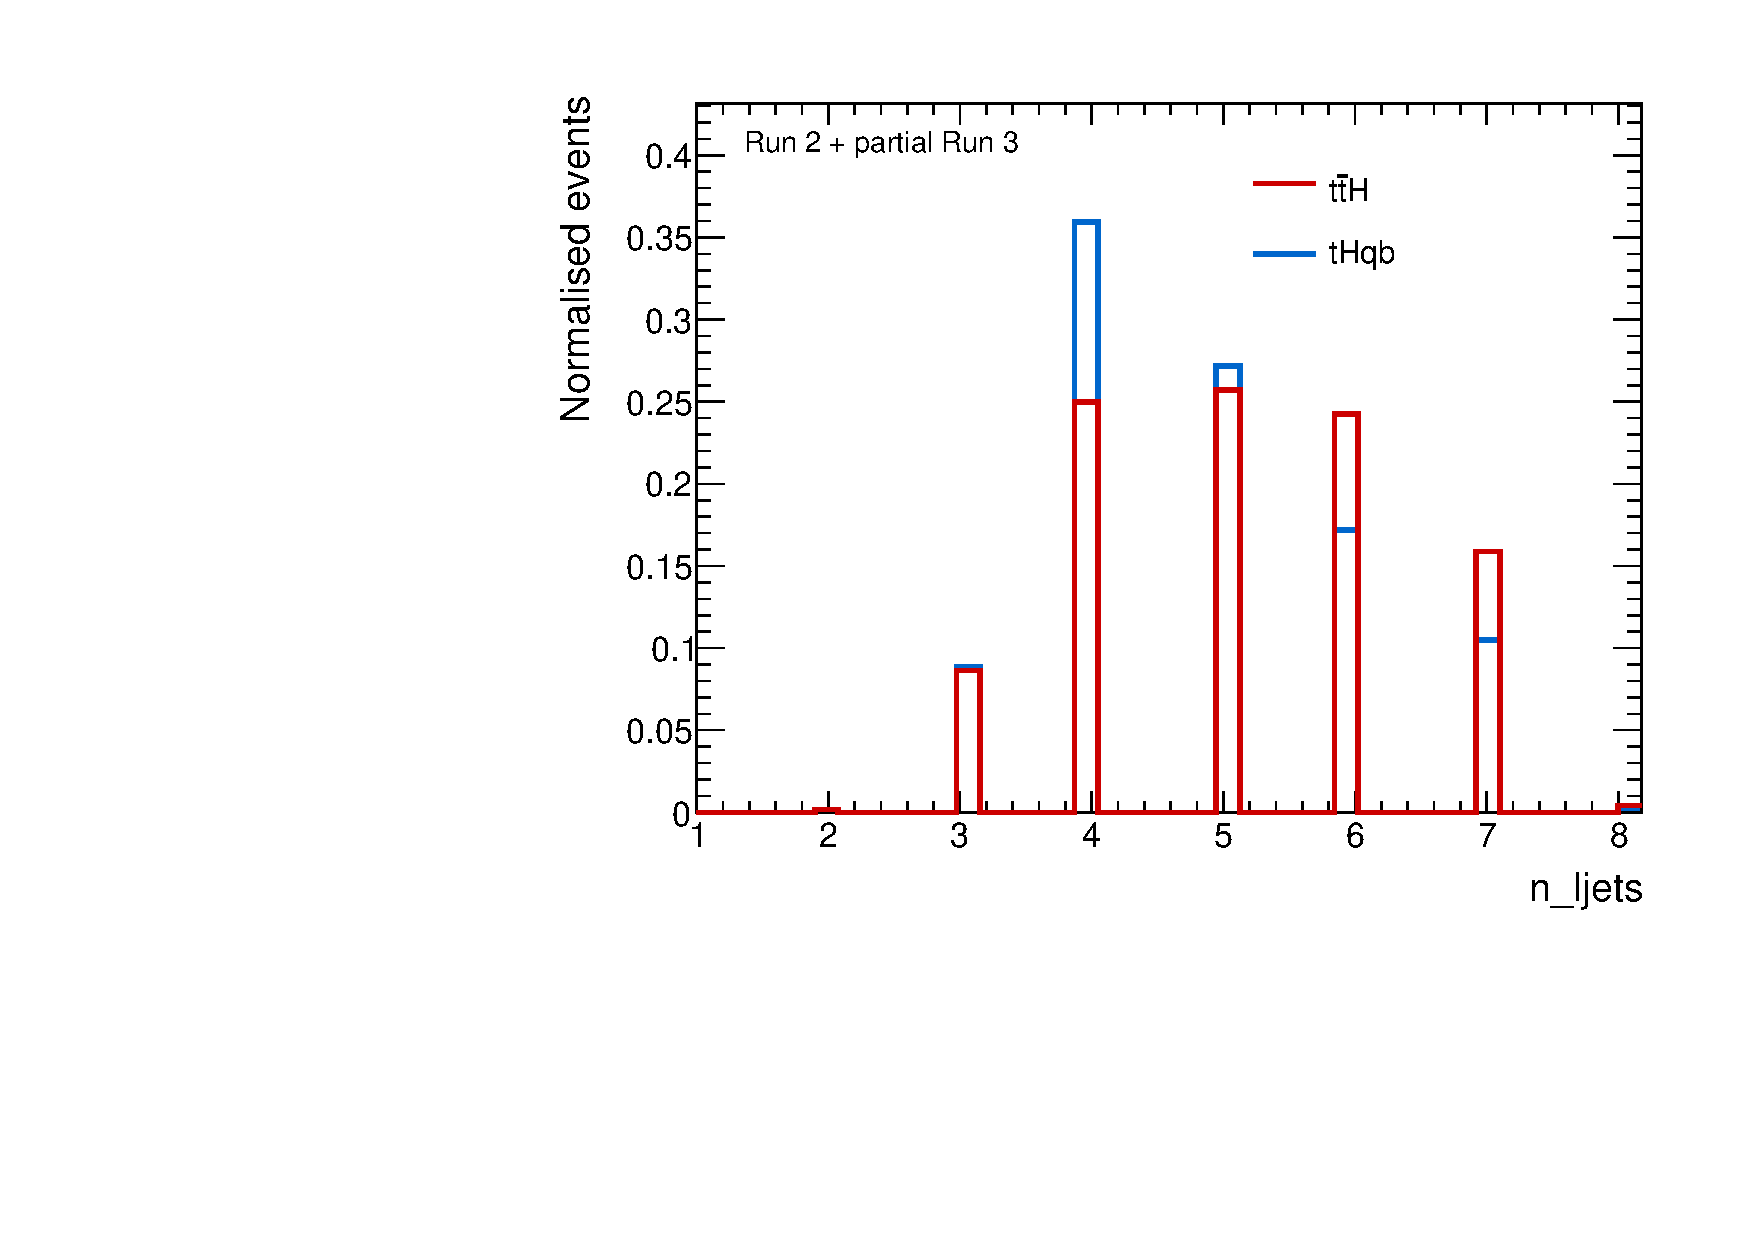
\includegraphics[width=\textwidth]{images/plots_tH_tHqb_for_thesis/n_ljets_signals_ATLAS.pdf}
    \caption{$n_{\text{ljets}}$}
    \label{fig:n_ljets}
  \end{subfigure}
  \hfill
  \begin{subfigure}[b]{0.45\textwidth}
    \centering
    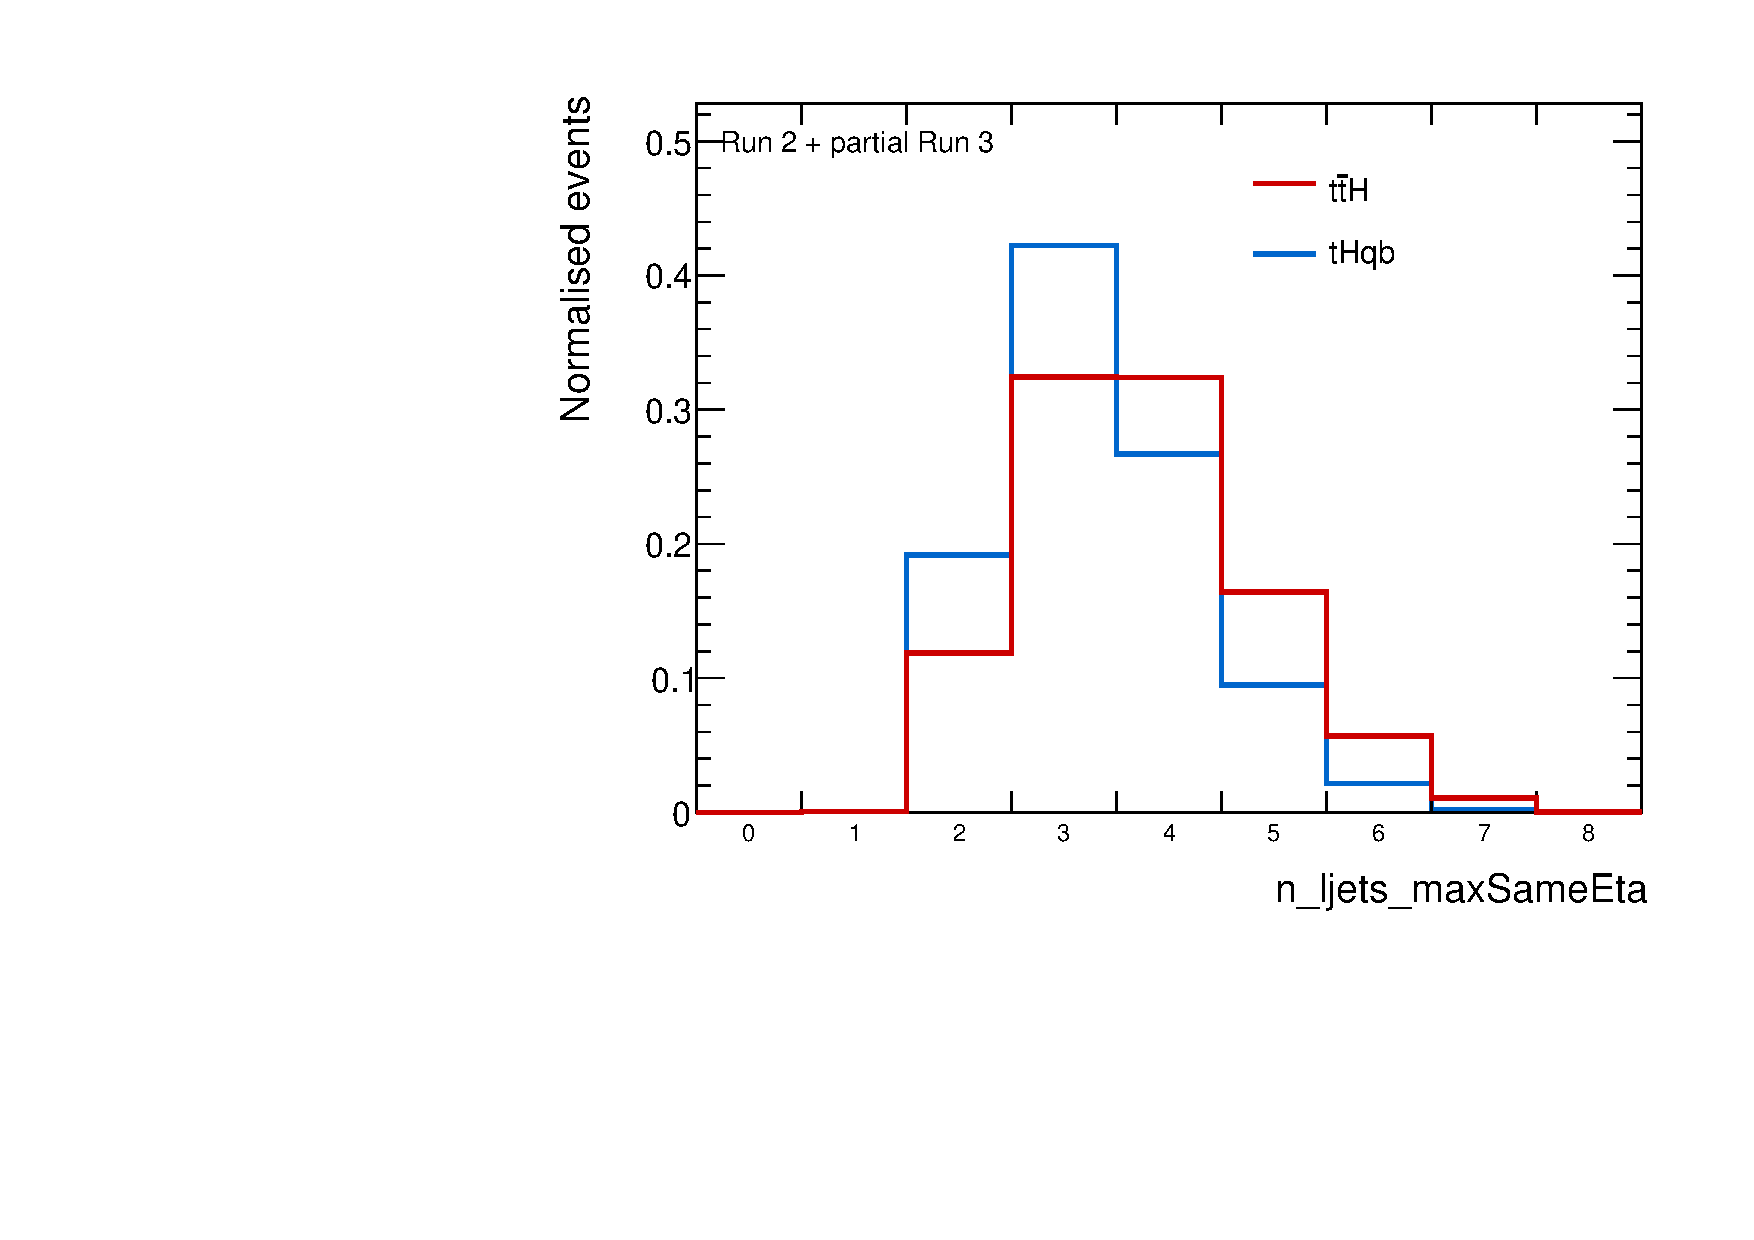
\includegraphics[width=\textwidth]{images/plots_tH_tHqb_for_thesis/n_ljets_maxSameEta_signals_ATLAS.pdf}
    \caption{$n_{\text{ljets}}^{\text{same }\eta}$}
    \label{fig:n_ljets_maxSameEta}
  \end{subfigure}

  % 2a fila
  \vskip\baselineskip
  \begin{subfigure}[b]{0.45\textwidth}
    \centering
    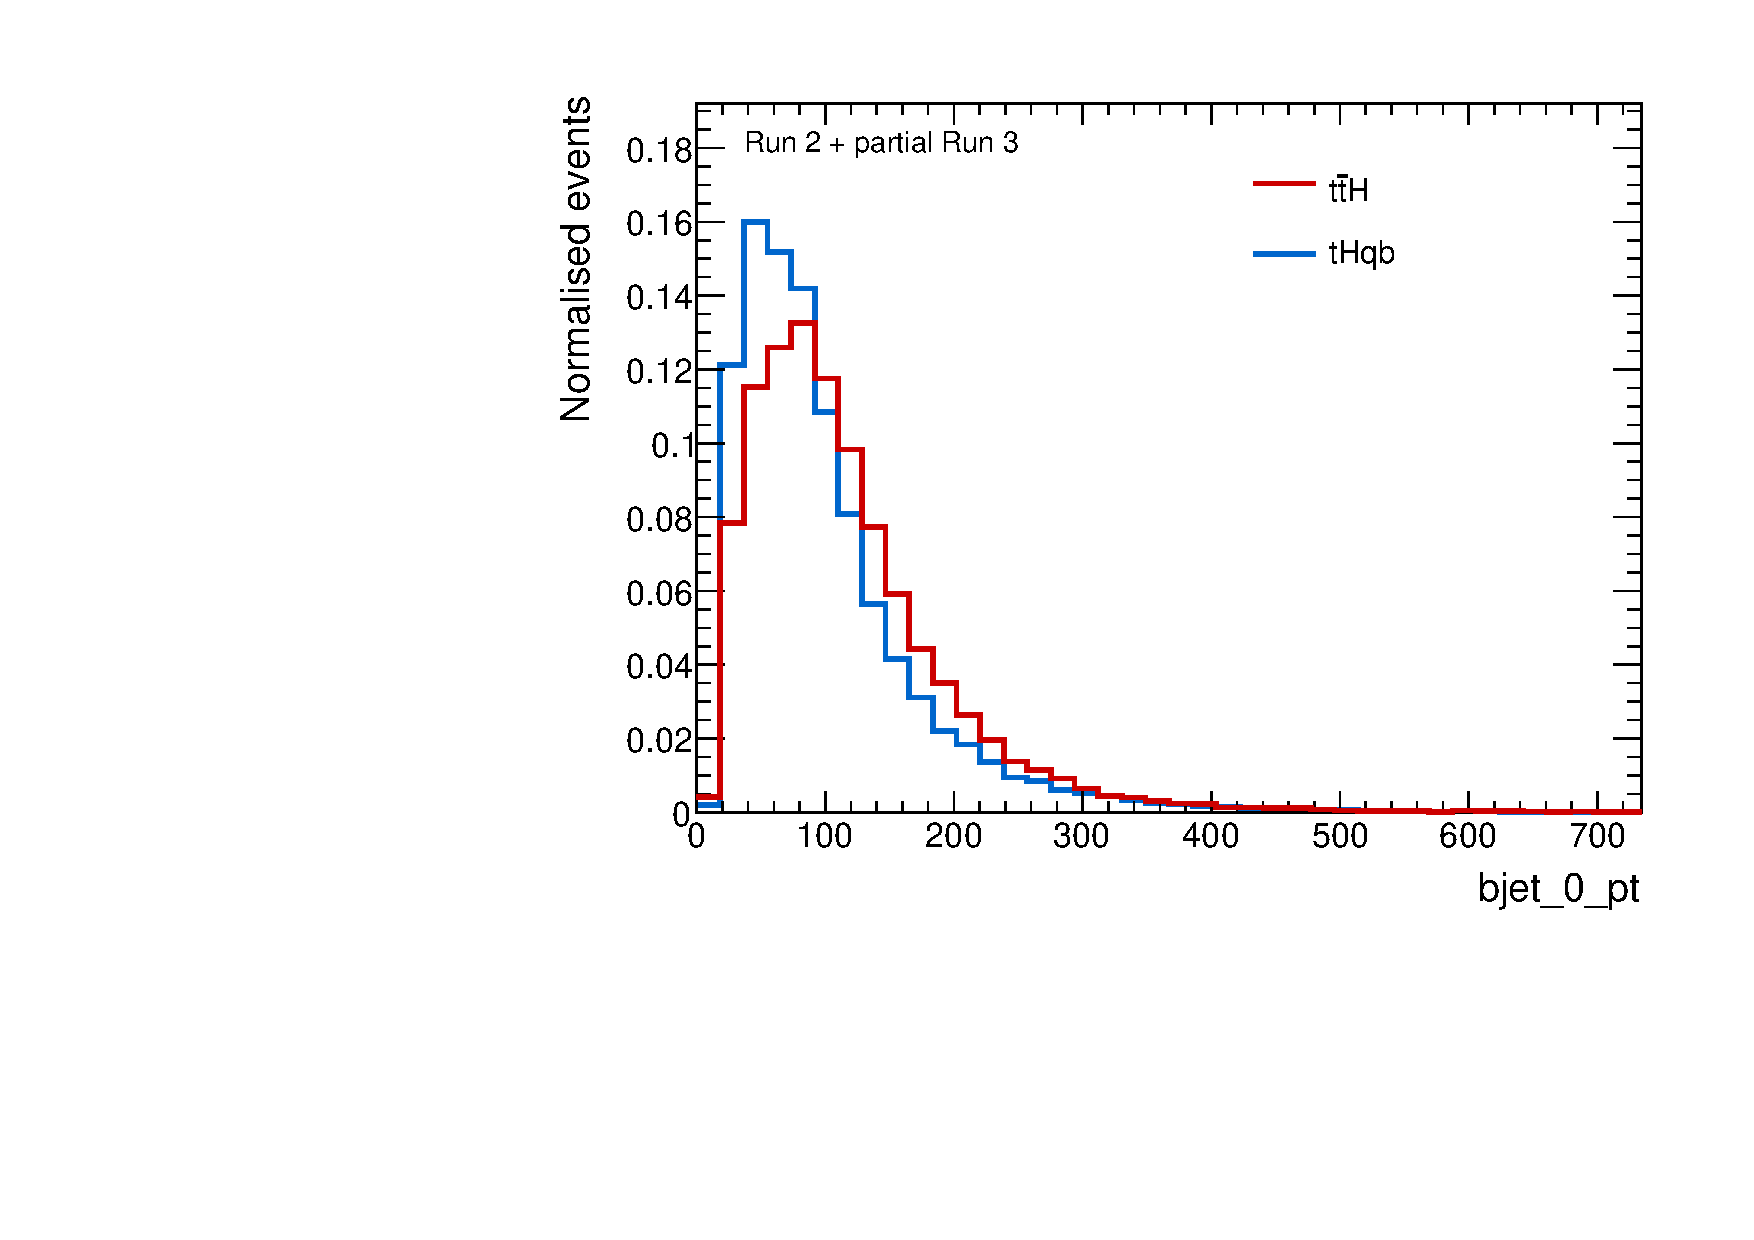
\includegraphics[width=\textwidth]{images/plots_tH_tHqb_for_thesis/bjet_0_pt_signals_ATLAS.pdf}
    \caption{$\eta$ of the leading $b$-jet}
    \label{fig:bjet0_eta}
  \end{subfigure}
  \hfill
  \begin{subfigure}[b]{0.45\textwidth}
    \centering
    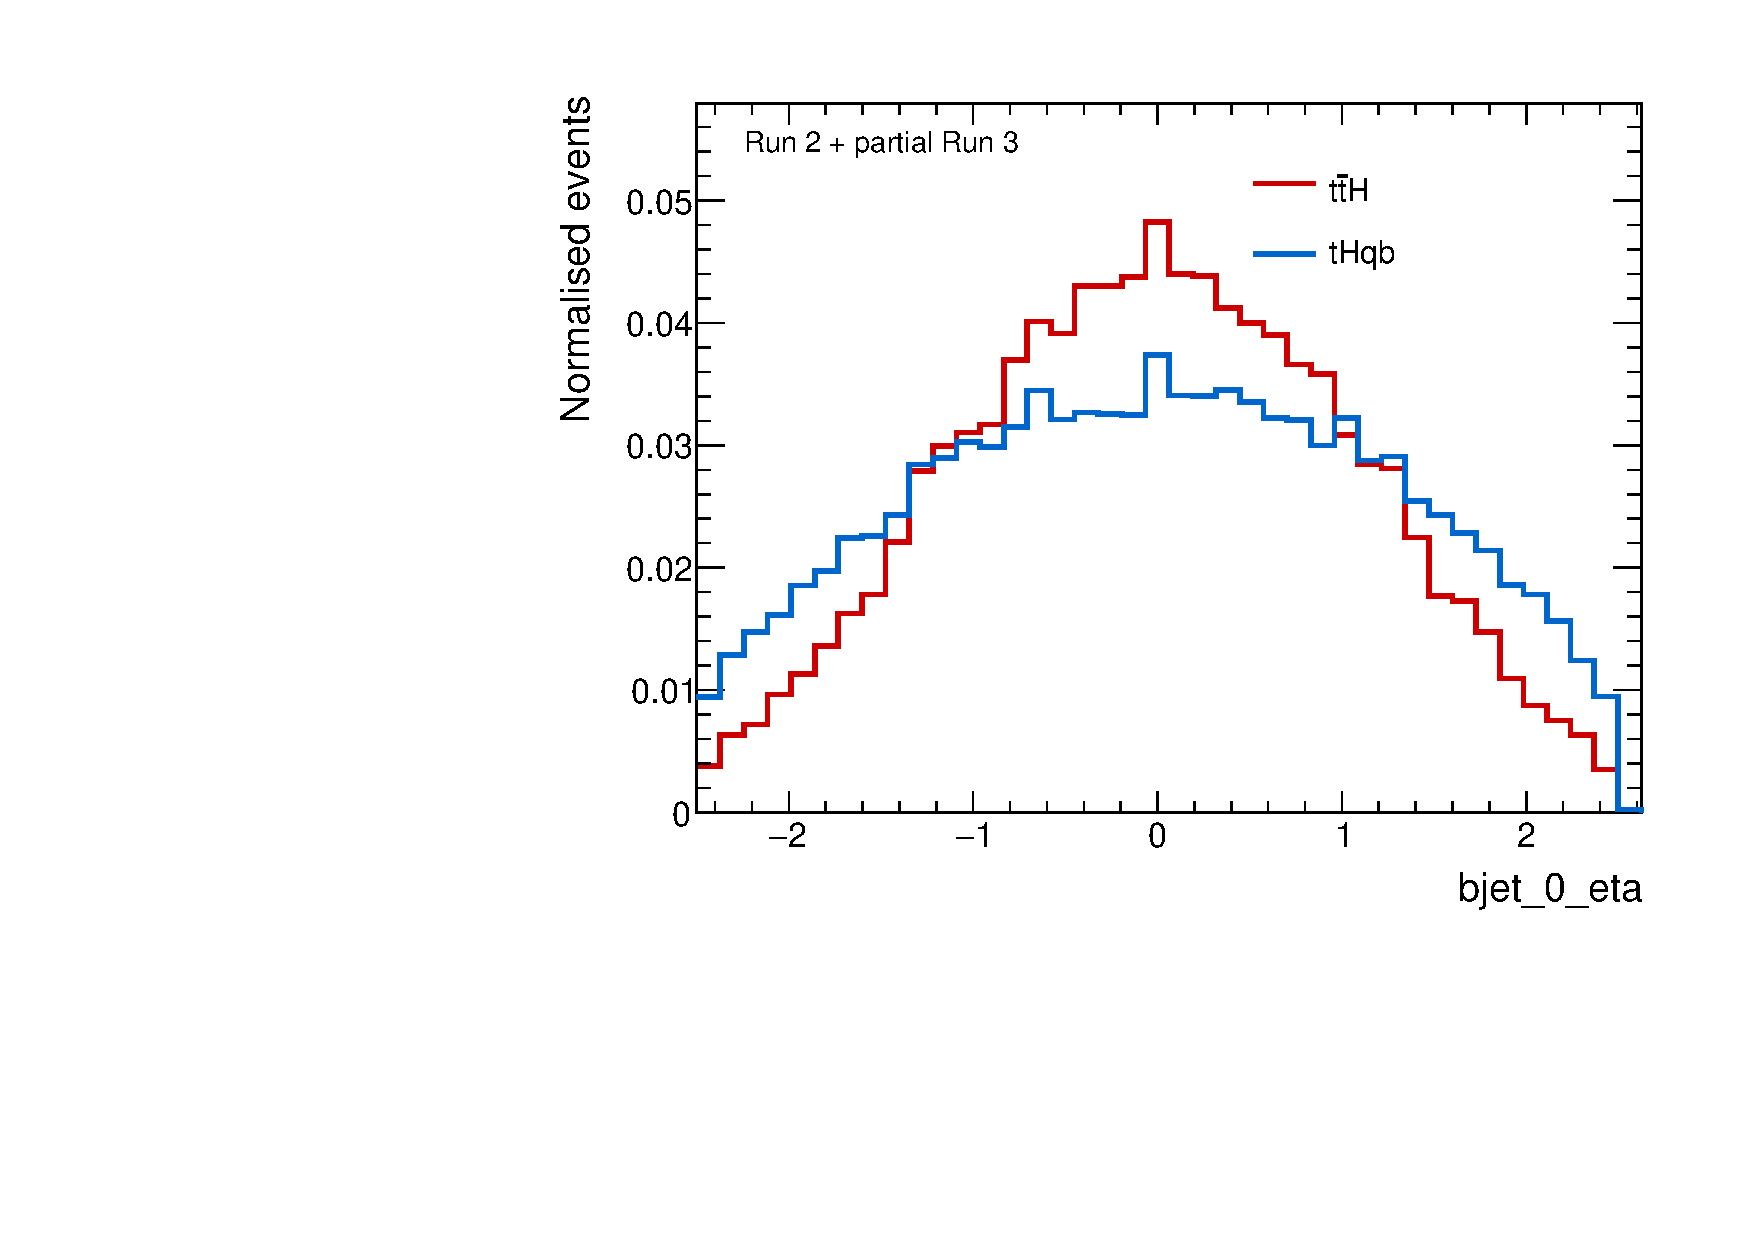
\includegraphics[width=\textwidth]{images/plots_tH_tHqb_for_thesis/bjet_0_eta_signals_ATLAS.pdf}
    \caption{$p_{\mathrm{T}}$ of the leading $b$-jet}
    \label{fig:bjet0_pt}
  \end{subfigure}

  \caption{Distributions of additional input variables used in the BDT training, shown for simulated \thqb and \ttH events after preselection cuts. 
  The observables exploit differences in the origin and kinematics of jets and $b$-jets in the two processes. 
  }
  \label{fig:th_vs_tth_1}
\end{figure}


% =========================
% Segunda figura (4 vars)
% =========================
\begin{figure}[htbp]
  \centering
  % 1a fila
  \begin{subfigure}[b]{0.45\textwidth}
    \centering
    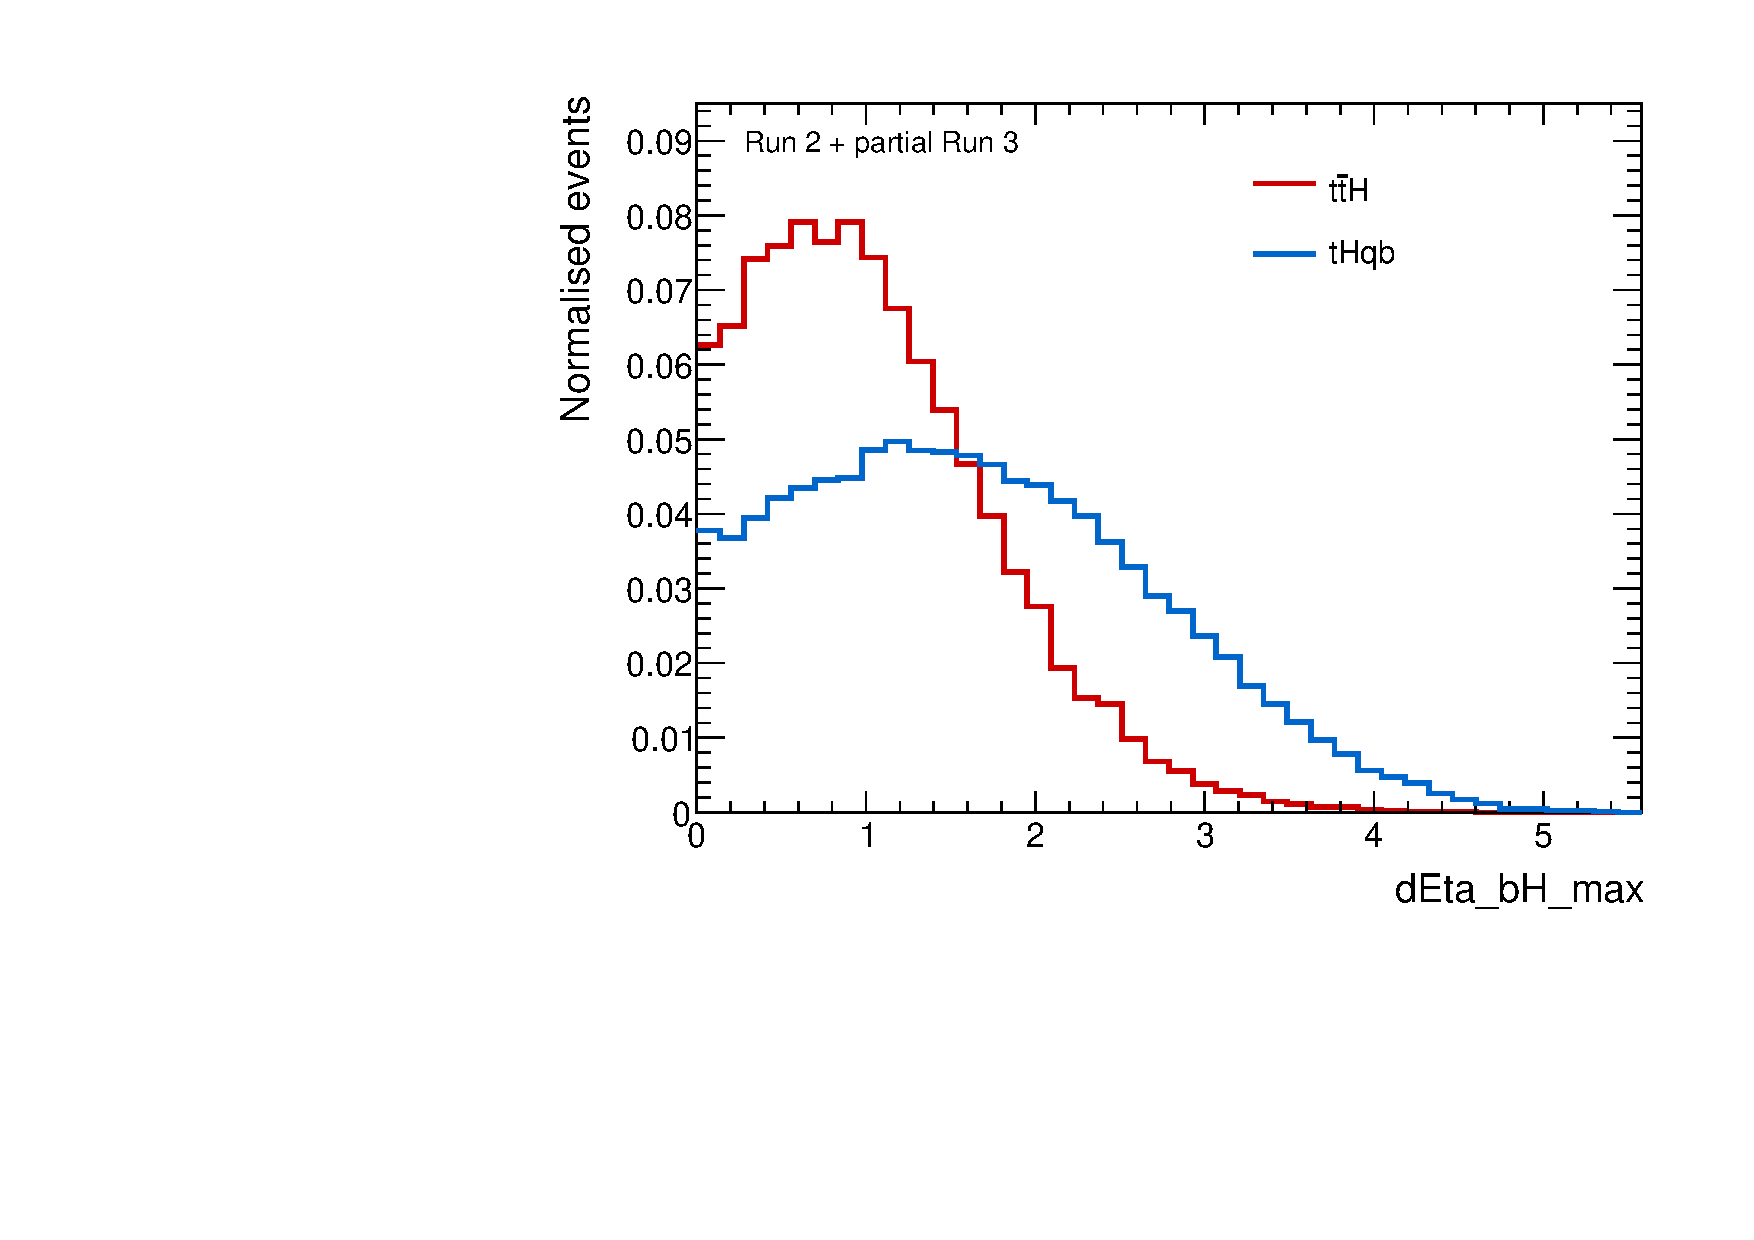
\includegraphics[width=\textwidth]{images/plots_tH_tHqb_for_thesis/dEta_bH_max_signals_ATLAS.pdf}
    \caption{Max.\ $\Delta \eta$ between $H$ decay products and any $b$-jet}
    \label{fig:dEta_bH_max}
  \end{subfigure}
  \hfill
  \begin{subfigure}[b]{0.45\textwidth}
    \centering
    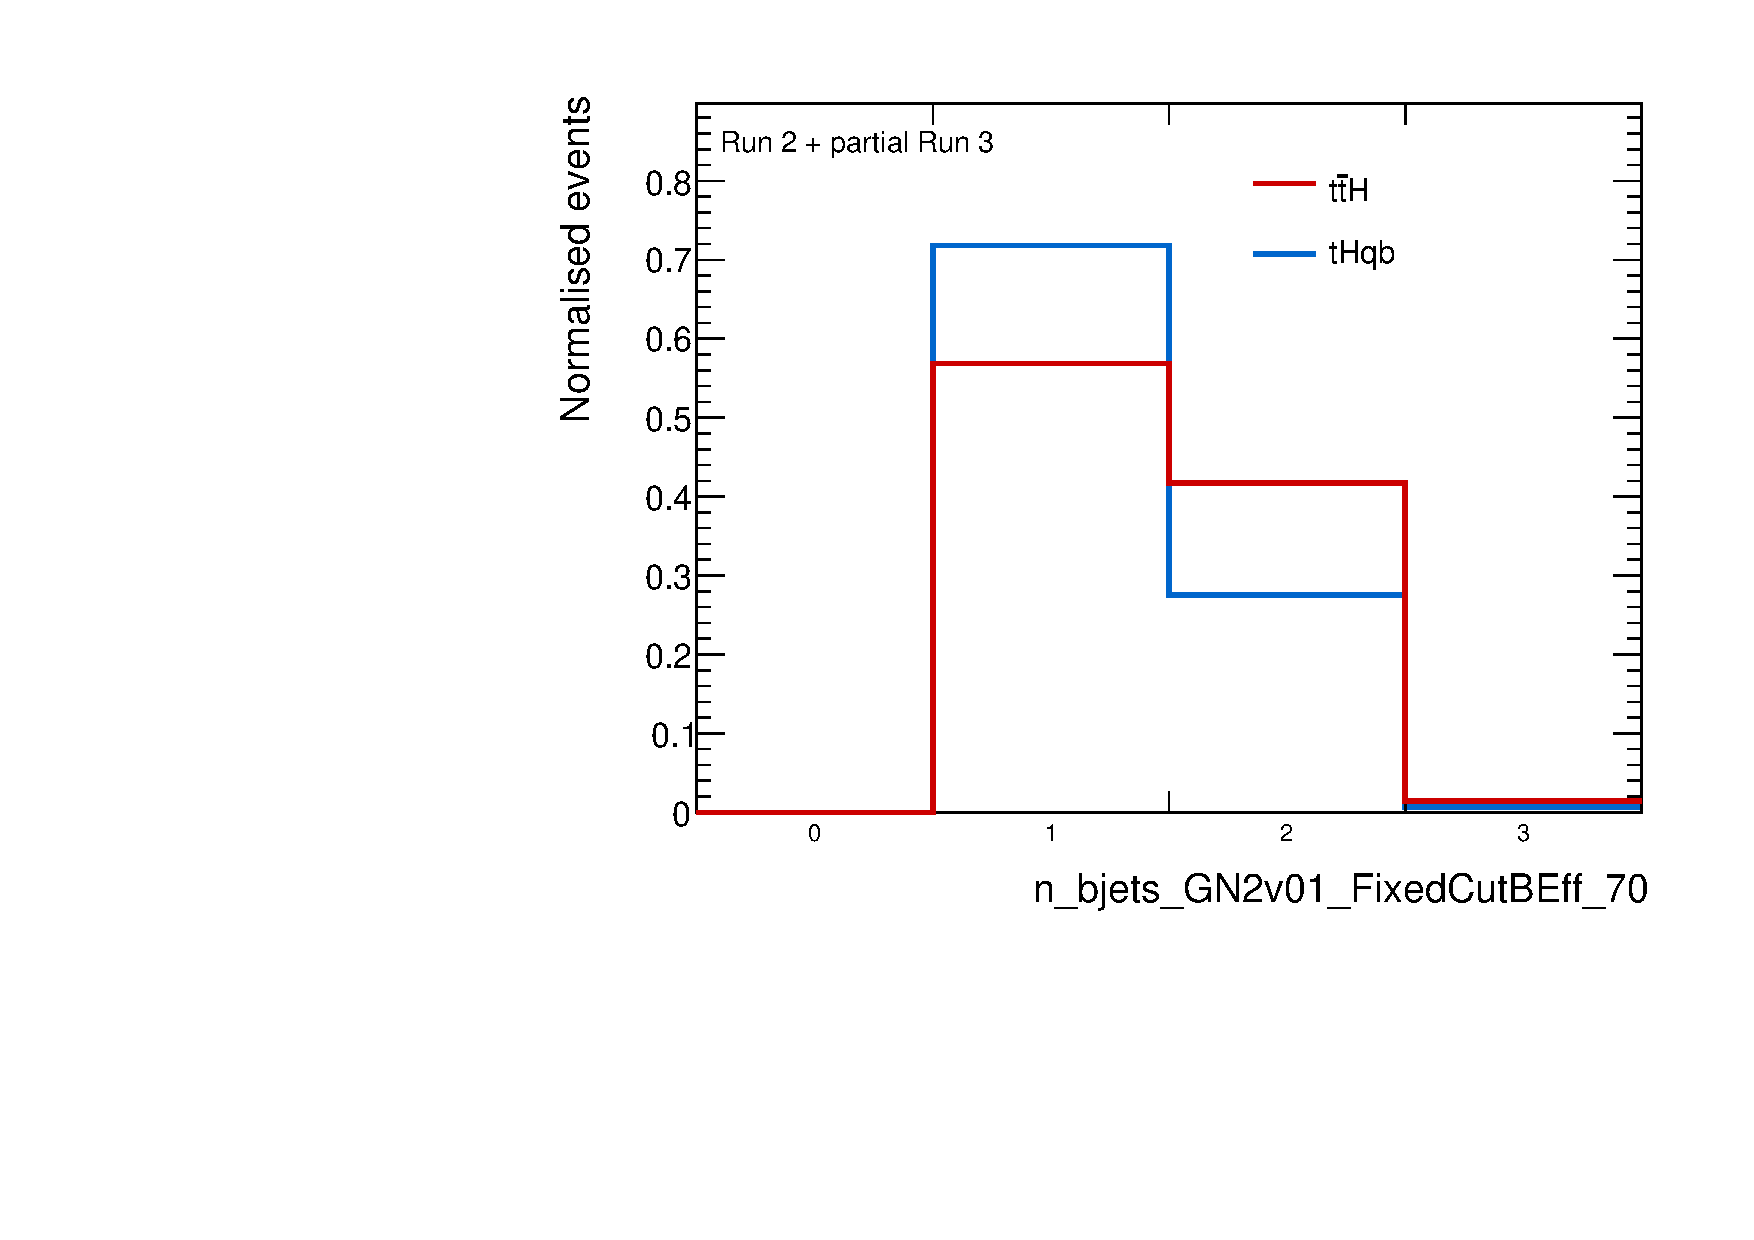
\includegraphics[width=\textwidth]{images/plots_tH_tHqb_for_thesis/n_bjets_GN2v01_FixedCutBEff_70_signals_ATLAS.pdf}
    \caption{$b$-jet multiplicity}
    \label{fig:n_bjets}
  \end{subfigure}

  % 2a fila
  \vskip\baselineskip
  \begin{subfigure}[b]{0.45\textwidth}
    \centering
    \includegraphics[width=\textwidth]{images/plots_tH_tHqb_for_thesis/dEta_lb_max_signals_ATLAS.pdf}
    \caption{Max.\ $\Delta \eta$ between any light jet and $b$-jet}
    \label{fig:dEta_lb_max}
  \end{subfigure}
  \hfill
  \begin{subfigure}[b]{0.45\textwidth}
    \centering
    \includegraphics[width=\textwidth]{images/plots_tH_tHqb_for_thesis/m_ll_max_signals_ATLAS.pdf}
    \caption{Largest invariant mass of two light jets}
    \label{fig:m_ll_max}
  \end{subfigure}

  \caption{Distributions of additional input variables used in the BDT training, shown for simulated \thqb and \ttH events after preselection cuts. 
  The observables exploit differences in the origin and kinematics of jets and $b$-jets in the two processes. 
  }
  \label{fig:th_vs_tth_2}
\end{figure}

Finally, Figures~\ref{th_tth_vars_tmva_1}-~\ref{th_tth_vars_tmva_3} show, analogously to what was presented in Section~\ref{sec:tth_mva}, the distributions of all variables employed in this new training for the four event classes under consideration.

\begin{figure}[htbp]
  \centering
  % Primera figura
  \begin{subfigure}{0.95\linewidth}
    \centering
    \includegraphics[width=\linewidth]{images/plots_tH_tHqb_for_thesis/variables_id_c1.png}
  \end{subfigure}
  \vspace{0.5cm} % Espacio vertical entre las dos
  % Segunda figura
  \begin{subfigure}{0.95\linewidth}
    \centering
    \includegraphics[width=\linewidth]{images/plots_tH_tHqb_for_thesis/variables_id_c2.png}
  \end{subfigure}
  \caption{Input variables for the multiclass BDT training for \thtt + \ttHtt. Preselection requirements used for the training are included.}
  \label{th_tth_vars_tmva_1}
  \end{figure}

  \begin{figure}[htbp]
    \centering
  % Segunda figura
  \begin{subfigure}{0.95\linewidth}
    \centering
    \includegraphics[width=\linewidth]{images/plots_tH_tHqb_for_thesis/variables_id_c3.png}
  \end{subfigure}
  \vspace{0.5cm} % Espacio vertical entre las dos
  % Segunda figura
  \begin{subfigure}{0.95\linewidth}
    \centering
    \includegraphics[width=\linewidth]{images/plots_tH_tHqb_for_thesis/variables_id_c4.png}
  \end{subfigure}
  \vspace{0.5cm} % Espacio vertical entre las dos
  % Segunda figura
  \caption{Input variables for the multiclass BDT training for \thtt + \ttHtt. Preselection requirements used for the training are included.}
  \label{th_tth_vars_tmva_2}
  \end{figure}

  \begin{figure}[htbp]
    \centering
    \includegraphics[width=0.95\linewidth]{images/plots_tH_tHqb_for_thesis/variables_id_c5.png}
  \caption{Input variables for the multiclass BDT training for \thtt + \ttHtt. Preselection requirements used for the training are included.}
  \label{th_tth_vars_tmva_3}
\end{figure}

It is worth noting that in this case the \mmc is indeed included as an input variable in the BDT training. The reasons behind this choice will be discussed later in Section~\ref{new_categorization}.

\subsubsection*{Data-MC modelling}


\begin{figure}[htbp]
  \centering
  % Ajusta el espacio horizontal entre paneles (columna a columna)
  \setlength{\tabcolsep}{1.5pt}
  \renewcommand{\arraystretch}{0}

  \begin{tabular}{@{}c c c@{}}
    \includegraphics[width=0.33\textwidth]{images/plots_modelling_run2_run3_variables/run_3_tth/plot_ditau_dr_hh_tth_22_23_24.pdf} &
    \includegraphics[width=0.33\textwidth]{images/plots_modelling_run2_run3_variables/run_3_tth/plot_ditau_deta_hh_tth_22_23_24.pdf} &
    \includegraphics[width=0.33\textwidth]{images/plots_modelling_run2_run3_variables/run_3_tth/plot_met_reco_et_hh_tth_22_23_24.pdf} \\[4pt]
    \includegraphics[width=0.33\textwidth]{images/plots_modelling_run2_run3_variables/run_3_tth/plot_mWbest_hh_tth_22_23_24.pdf} &
    \includegraphics[width=0.33\textwidth]{images/plots_modelling_run2_run3_variables/run_3_tth/plot_SumPtBjet_hh_tth_22_23_24.pdf} &
    \includegraphics[width=0.33\textwidth]{images/plots_modelling_run2_run3_variables/run_3_tth/plot_mTopWbest_hh_tth_22_23_24.pdf} \\[4pt]
    \includegraphics[width=0.33\textwidth]{images/plots_modelling_run2_run3_variables/run_3_tth/plot_ditau_pt_hh_tth_22_23_24.pdf} &
    \includegraphics[width=0.33\textwidth]{images/plots_modelling_run2_run3_variables/run_3_tth/plot_jjdrmin_hh_tth_22_23_24.pdf} &
    \includegraphics[width=0.33\textwidth]{images/plots_modelling_run2_run3_variables/run_3_tth/plot_min_dr_btau_hh_tth_22_23_24.pdf}\\[4pt]
    \includegraphics[width=0.33\textwidth]{images/plots_modelling_run2_run3_variables/run_3_tth/plot_eta2_hh_tth_22_23_24.pdf} &
    \includegraphics[width=0.33\textwidth]{images/plots_modelling_run2_run3_variables/run_3_tth/plot_eta3_hh_tth_22_23_24.pdf} &
    \includegraphics[width=0.33\textwidth]{images/plots_modelling_run2_run3_variables/run_3_tth/plot_eta4_hh_tth_22_23_24.pdf}
  \end{tabular}

  \caption{Run-3 Data/MC modelling for the \thqb + \ttH BDT input variables at preselection level.}
  \label{tth_vars_modelling_run3_1}
\end{figure}

\begin{figure}[htbp]
  \centering
  % Ajusta el espacio horizontal entre paneles (columna a columna)
  \setlength{\tabcolsep}{1.5pt}
  \renewcommand{\arraystretch}{0}

  \begin{tabular}{@{}c c c@{}}
    \includegraphics[width=0.33\textwidth]{images/plots_modelling_run2_run3_variables/run_3_tth/plot_tau_1_pt_hh_tth_22_23_24.pdf} &
    \includegraphics[width=0.33\textwidth]{images/plots_modelling_run2_run3_variables/run_3_tth/plot_SumPtBjet_hh_tth_22_23_24.pdf} &
    \includegraphics[width=0.33\textwidth]{images/plots_modelling_run2_run3_variables/run_3_tth/plot_tau_0_eta_hh_tth_22_23_24.pdf} \\[4pt]
    \includegraphics[width=0.33\textwidth]{images/plots_modelling_run2_run3_variables/run_3_tth/plot_jet_1_eta_hh_tth_22_23_24.pdf} &
    \includegraphics[width=0.33\textwidth]{images/plots_modelling_run2_run3_variables/run_3_tth/plot_jet_0_eta_hh_tth_22_23_24.pdf} &
    \includegraphics[width=0.33\textwidth]{images/plots_modelling_run2_run3_variables/run_3_tth/plot_ditau_met_min_dphi_hh_tth_22_23_24.pdf} \\[4pt]
    \includegraphics[width=0.33\textwidth]{images/plots_modelling_run2_run3_variables/run_3_tth/plot_ratio01_hh_tth_22_23_24.pdf} &
    \includegraphics[width=0.33\textwidth]{images/plots_modelling_run2_run3_variables/run_3_tth/plot_ratio12_hh_tth_22_23_24.pdf} &
    \includegraphics[width=0.33\textwidth]{images/plots_modelling_run2_run3_variables/run_3_tth/plot_ratio13_hh_tth_22_23_24.pdf} \\[4pt]
    \includegraphics[width=0.33\textwidth]{images/plots_modelling_run2_run3_variables/run_3_tth/plot_n_ljets_hh_tth_22_23_24.pdf} &
    \includegraphics[width=0.33\textwidth]{images/plots_modelling_run2_run3_variables/run_3_tth/plot_n_ljets_maxSameEta_hh_tth_22_23_24.pdf} &
    \includegraphics[width=0.33\textwidth]{images/plots_modelling_run2_run3_variables/run_3_tth/plot_bjet_0_eta_hh_tth_22_23_24.pdf}
  \end{tabular}

  \caption{Run-3 Data/MC modelling for the \thqb + \ttH BDT input variables at preselection level.}
  \label{tth_vars_modelling_run3_2}
\end{figure}

\begin{figure}[htbp]
  \centering
  % Espacio horizontal entre columnas del tabular
  \setlength{\tabcolsep}{1.5pt}
  \renewcommand{\arraystretch}{1.0}

  \begin{tabular}{@{}c c c@{}}
    \includegraphics[width=0.33\textwidth]{images/plots_modelling_run2_run3_variables/run_3_tth/plot_bjet_0_pt_hh_tth_22_23_24.pdf} &
    \includegraphics[width=0.33\textwidth]{images/plots_modelling_run2_run3_variables/run_3_tth/plot_dEta_bH_max_hh_tth_22_23_24.pdf} &
    \includegraphics[width=0.33\textwidth]{images/plots_modelling_run2_run3_variables/run_3_tth/plot_n_bjets_GN2v01_FixedCutBEff_70_hh_tth_22_23_24.pdf}
    \\[4pt]
    \multicolumn{3}{c}{%
      \includegraphics[width=0.33\textwidth]{images/plots_modelling_run2_run3_variables/run_3_tth/plot_dEta_lb_max_hh_tth_22_23_24.pdf}%
      \hspace{1.5pt}%
      \includegraphics[width=0.33\textwidth]{images/plots_modelling_run2_run3_variables/run_3_tth/plot_m_ll_max_hh_tth_22_23_24.pdf}%
    }\\
  \end{tabular}

  \caption{Run-3 Data/MC modelling for the \thqb + \ttH BDT input variables at preselection level.}
  \label{tth_vars_modelling_run3_2}
\end{figure}



%%%%%%%%%%%%%%%%%%%%%%%%%%%%%%%%%%%%%%%%%%%% RUN2 %%%%%%%%%%%%%%%%%%%%%%%%%%%%%%%%%%%%%%%%%%%%%%%%%%%%%%%%%%%%%%%%%%%%%%%%%%%

\begin{figure}[htbp]
  \centering
  % Ajusta el espacio horizontal entre paneles (columna a columna)
  \setlength{\tabcolsep}{1.5pt}
  \renewcommand{\arraystretch}{0}

  \begin{tabular}{@{}c c c@{}}
    \includegraphics[width=0.33\textwidth]{images/plots_modelling_run2_run3_variables/run_2_tth/plot_ditau_dr_hh_tth_15_16_17_18.pdf} &
    \includegraphics[width=0.33\textwidth]{images/plots_modelling_run2_run3_variables/run_2_tth/plot_ditau_deta_hh_tth_15_16_17_18.pdf} &
    \includegraphics[width=0.33\textwidth]{images/plots_modelling_run2_run3_variables/run_2_tth/plot_met_reco_et_hh_tth_15_16_17_18.pdf} \\[4pt]
    \includegraphics[width=0.33\textwidth]{images/plots_modelling_run2_run3_variables/run_2_tth/plot_mWbest_hh_tth_15_16_17_18.pdf} &
    \includegraphics[width=0.33\textwidth]{images/plots_modelling_run2_run3_variables/run_2_tth/plot_SumPtBjet_hh_tth_15_16_17_18.pdf} &
    \includegraphics[width=0.33\textwidth]{images/plots_modelling_run2_run3_variables/run_2_tth/plot_mTopWbest_hh_tth_15_16_17_18.pdf} \\[4pt]
    \includegraphics[width=0.33\textwidth]{images/plots_modelling_run2_run3_variables/run_2_tth/plot_ditau_pt_hh_tth_15_16_17_18.pdf} &
    \includegraphics[width=0.33\textwidth]{images/plots_modelling_run2_run3_variables/run_2_tth/plot_jjdrmin_hh_tth_15_16_17_18.pdf} &
    \includegraphics[width=0.33\textwidth]{images/plots_modelling_run2_run3_variables/run_2_tth/plot_min_dr_btau_hh_tth_15_16_17_18.pdf}\\[4pt]
    \includegraphics[width=0.33\textwidth]{images/plots_modelling_run2_run3_variables/run_2_tth/plot_eta2_hh_tth_15_16_17_18.pdf} &
    \includegraphics[width=0.33\textwidth]{images/plots_modelling_run2_run3_variables/run_2_tth/plot_eta3_hh_tth_15_16_17_18.pdf} &
    \includegraphics[width=0.33\textwidth]{images/plots_modelling_run2_run3_variables/run_2_tth/plot_eta4_hh_tth_15_16_17_18.pdf}
  \end{tabular}

  \caption{Run-2 Data/MC modelling for the \thqb + \ttH BDT input variables at preselection level.}
  \label{tth_vars_modelling_run3_1}
\end{figure}

\begin{figure}[htbp]
  \centering
  % Ajusta el espacio horizontal entre paneles (columna a columna)
  \setlength{\tabcolsep}{1.5pt}
  \renewcommand{\arraystretch}{0}

  \begin{tabular}{@{}c c c@{}}
    \includegraphics[width=0.33\textwidth]{images/plots_modelling_run2_run3_variables/run_2_tth/plot_tau_1_pt_hh_tth_15_16_17_18.pdf} &
    \includegraphics[width=0.33\textwidth]{images/plots_modelling_run2_run3_variables/run_2_tth/plot_SumPtBjet_hh_tth_15_16_17_18.pdf} &
    \includegraphics[width=0.33\textwidth]{images/plots_modelling_run2_run3_variables/run_2_tth/plot_tau_0_eta_hh_tth_15_16_17_18.pdf} \\[4pt]
    \includegraphics[width=0.33\textwidth]{images/plots_modelling_run2_run3_variables/run_2_tth/plot_jet_1_eta_hh_tth_15_16_17_18.pdf} &
    \includegraphics[width=0.33\textwidth]{images/plots_modelling_run2_run3_variables/run_2_tth/plot_jet_0_eta_hh_tth_15_16_17_18.pdf} &
    \includegraphics[width=0.33\textwidth]{images/plots_modelling_run2_run3_variables/run_2_tth/plot_ditau_met_min_dphi_hh_tth_15_16_17_18.pdf} \\[4pt]
    \includegraphics[width=0.33\textwidth]{images/plots_modelling_run2_run3_variables/run_2_tth/plot_ratio01_hh_tth_15_16_17_18.pdf} &
    \includegraphics[width=0.33\textwidth]{images/plots_modelling_run2_run3_variables/run_2_tth/plot_ratio12_hh_tth_15_16_17_18.pdf} &
    \includegraphics[width=0.33\textwidth]{images/plots_modelling_run2_run3_variables/run_2_tth/plot_ratio13_hh_tth_15_16_17_18.pdf} \\[4pt]
    \includegraphics[width=0.33\textwidth]{images/plots_modelling_run2_run3_variables/run_2_tth/plot_n_ljets_hh_tth_15_16_17_18.pdf} &
    \includegraphics[width=0.33\textwidth]{images/plots_modelling_run2_run3_variables/run_2_tth/plot_n_ljets_maxSameEta_hh_tth_15_16_17_18.pdf} &
    \includegraphics[width=0.33\textwidth]{images/plots_modelling_run2_run3_variables/run_2_tth/plot_bjet_0_eta_hh_tth_15_16_17_18.pdf}
  \end{tabular}

  \caption{Run-2 Data/MC modelling for the \thqb + \ttH BDT input variables at preselection level.}
  \label{tth_vars_modelling_run3_2}
\end{figure}

\begin{figure}[htbp]
  \centering
  % Espacio horizontal entre columnas del tabular
  \setlength{\tabcolsep}{1.5pt}
  \renewcommand{\arraystretch}{1.0}

  \begin{tabular}{@{}c c c@{}}
    \includegraphics[width=0.33\textwidth]{images/plots_modelling_run2_run3_variables/run_2_tth/plot_bjet_0_pt_hh_tth_15_16_17_18.pdf} &
    \includegraphics[width=0.33\textwidth]{images/plots_modelling_run2_run3_variables/run_2_tth/plot_dEta_bH_max_hh_tth_15_16_17_18.pdf} &
    \includegraphics[width=0.33\textwidth]{images/plots_modelling_run2_run3_variables/run_2_tth/plot_n_bjets_GN2v01_FixedCutBEff_70_hh_tth_15_16_17_18.pdf}
    \\[4pt]
    \multicolumn{3}{c}{%
      \includegraphics[width=0.33\textwidth]{images/plots_modelling_run2_run3_variables/run_2_tth/plot_dEta_lb_max_hh_tth_15_16_17_18.pdf}%
      \hspace{1.5pt}%
      \includegraphics[width=0.33\textwidth]{images/plots_modelling_run2_run3_variables/run_2_tth/plot_m_ll_max_hh_tth_15_16_17_18.pdf}%
    }\\
  \end{tabular}

  \caption{Run-2 Data/MC modelling for the \thqb + \ttH BDT input variables at preselection level.}
  \label{tth_vars_modelling_run3_2}
\end{figure}


\subsubsection*{Data-MC modelling}

\begin{figure}[htbp]
  \centering
  \begin{subfigure}[b]{0.49\textwidth}
    \centering
    \includegraphics[width=\textwidth]{images/plots_tH_tHqb_for_thesis/BDTScore_tH_ATLAS.pdf}
    \caption{}
    \label{fig:bdtscore_th}
  \end{subfigure}
  \hfill
  \begin{subfigure}[b]{0.49\textwidth}
    \centering
    \includegraphics[width=\textwidth]{images/plots_tH_tHqb_for_thesis/BDTScore_ttH_ATLAS.pdf}
    \caption{}
    \label{fig:bdtscore_tth}
  \end{subfigure}

  \vskip\baselineskip

  \begin{subfigure}[b]{0.49\textwidth}
    \centering
    \includegraphics[width=\textwidth]{images/plots_tH_tHqb_for_thesis/BDTScore_bkgZ_ATLAS.pdf}
    \caption{}
    \label{fig:bdtscore_bkgZ}
  \end{subfigure}
  \hfill
  \begin{subfigure}[b]{0.49\textwidth}
    \centering
    \includegraphics[width=\textwidth]{images/plots_tH_tHqb_for_thesis/BDTScore_bkgtt_ATLAS.pdf}
    \caption{}
    \label{fig:bdtscore_bkgtt}
  \end{subfigure}

  \caption{Multiclass \thqb + \ttH BDT score distributions.}
  \label{highpt_scores}
\end{figure}



\begin{figure}[htbp]
  \centering
  \begin{subfigure}[b]{0.49\textwidth}
    \centering
    \includegraphics[width=\textwidth]{images/plots_modelling_run2_run3_variables/run_3_tth/plot_tth_th_multiclass_th_hh_tth_run3_sr_th_22_23_24.pdf}
    \caption{}
    \label{fig:overtrain_signal}
  \end{subfigure}
  \hfill
  \begin{subfigure}[b]{0.49\textwidth}
    \centering
    \includegraphics[width=\textwidth]{images/plots_modelling_run2_run3_variables/run_3_tth/plot_tth_th_multiclass_tth_hh_tth_run3_sr_tth_22_23_24.pdf}
    \caption{}
    \label{fig:overtrain_Z}
  \end{subfigure}

  \vskip\baselineskip

  \begin{subfigure}[b]{0.49\textwidth}
    \centering
    \includegraphics[width=\textwidth]{images/plots_modelling_run2_run3_variables/run_3_tth/plot_tth_th_multiclass_Z_hh_tth_run3_cr_Ztt_22_23_24.pdf}
    \caption{}
    \label{fig:overtrain_ttbar}
  \end{subfigure}
  \hfill
  \begin{subfigure}[b]{0.49\textwidth}
    \centering
    \includegraphics[width=\textwidth]{images/plots_modelling_run2_run3_variables/run_3_tth/plot_tth_th_multiclass_ttbar_hh_tth_run3_cr_ttbar_22_23_24.pdf}
    \caption{}
    \label{fig:overtrain_bkg}
  \end{subfigure}

  \caption{Run-3 Data/MC comparison for the Multiclass BDT scores.}
  \label{scores_modelling}
\end{figure}


\begin{figure}[htbp]
  \centering
  \begin{subfigure}[b]{0.49\textwidth}
    \centering
    \includegraphics[width=\textwidth]{images/plots_modelling_run2_run3_variables/run_2_tth/plot_tth_th_multiclass_th_hh_tth_run2_sr_th_15_16_17_18.pdf}
    \caption{}
    \label{fig:overtrain_signal}
  \end{subfigure}
  \hfill
  \begin{subfigure}[b]{0.49\textwidth}
    \centering
    \includegraphics[width=\textwidth]{images/plots_modelling_run2_run3_variables/run_2_tth/plot_tth_th_multiclass_tth_hh_tth_run2_sr_tth_15_16_17_18.pdf}
    \caption{}
    \label{fig:overtrain_Z}
  \end{subfigure}

  \vskip\baselineskip

  \begin{subfigure}[b]{0.49\textwidth}
    \centering
    \includegraphics[width=\textwidth]{images/plots_modelling_run2_run3_variables/run_2_tth/plot_tth_th_multiclass_Z_hh_tth_run2_cr_Ztt_15_16_17_18.pdf}
    \caption{}
    \label{fig:overtrain_ttbar}
  \end{subfigure}
  \hfill
  \begin{subfigure}[b]{0.49\textwidth}
    \centering
    \includegraphics[width=\textwidth]{images/plots_modelling_run2_run3_variables/run_2_tth/plot_tth_th_multiclass_ttbar_hh_tth_run2_cr_ttbar_15_16_17_18.pdf}
    \caption{}
    \label{fig:overtrain_bkg}
  \end{subfigure}

  \caption{Run-2 Data/MC comparison for the Multiclass BDT scores.}
  \label{scores_modelling}
\end{figure}


\subsection{Event categorization}
\label{new_categorization}

AQUI HABLAMOS DE LA MMC, QUE ENTRA EN EL TRAINING Y NINGUN OTRO SITIO (DEL FIT COMENTARLO EN EL FIT).
DECIR QUE OBVIAMENTE SE RECONSTRUYE COMO EN EL ANALISIS ANTERIOR, Y QUE DEL PT(H) NOS DA IGUAL PORQUE LO HACEMOS INCLUSIVO 
\section{Statistical fit}
\label{statistical_th_tth}


%% - events and object selection: (same trigger, objetos se reconstruyen y todo igual salvo GNTau ID y b-jets, events selection relajando a 5j1b), 
%% - Fakes background estimation (diciendo también antes, o aquí, que el resto de backgrounds se estiman como en el analisis anterior), 
%% - New MVA strategy for event categorization (4-class y todo el modeling y demás, y como se definen las regiones) ==> mencionar lo de que usamos los
%% BDT scores para el fit como input, la MMC no, la MMC ahora se mete en el training (mirar presentación 22 de julio de Ximo)
%% - Statistical Fit

